\documentclass[11pt,a4paper,notitlepage,fleqn,final]{article}

\usepackage{amsmath}
\usepackage{amsfonts}
\usepackage{amssymb}
\usepackage{libs/commath2}
\usepackage{xcolor}
\usepackage[hidelinks]{hyperref}
\usepackage[skins,theorems]{tcolorbox}
\usepackage{titlesec}
\usepackage{circuitikz}
\usepackage{pgfplots}
\usepackage{mathtools}
\usepackage[makeroom]{cancel}
\usepackage{mathrsfs}
\usepackage{wrapfig}
\usepackage{subcaption}
\usepackage{floatrow}
\usepackage{esint}
\usepackage{enumitem}
\usepackage{bm}
\usepackage{relsize}
\usepackage{xfrac}
\usepackage{comment}
\usepackage{siunitx}
\usepackage{MnSymbol}
\usepackage[obeyDraft]{todonotes}

\pgfplotsset{compat=1.13}
\usetikzlibrary{arrows.meta}
\usetikzlibrary{patterns}
\usetikzlibrary{decorations.pathmorphing,patterns}
\usetikzlibrary{decorations.markings}
\usetikzlibrary{backgrounds}
\usetikzlibrary{shapes.misc}
\usetikzlibrary{shapes.multipart}
\usetikzlibrary{snakes}
\usetikzlibrary{fadings}
\usetikzlibrary{intersections}
\usetikzlibrary{arrows.meta}
\usetikzlibrary{calc}
\usetikzlibrary{matrix}

\tikzset{cross/.style={cross out, draw,
        minimum size=2*(#1-\pgflinewidth),
        inner sep=0pt, outer sep=0pt}}
\tikzset{
    mark position/.style args={#1(#2)}{
        postaction={
            decorate,
            decoration={
            	post length=1mm, % ??? Magic to fix "Dimension
            	pre length=1mm, % ???  too large" errors.
                markings,
                mark=at position #1 with \coordinate (#2);
            }
        }
    }
}

\pgfmathdeclarefunction{sinc}{1}{%
	\pgfmathparse{abs(#1)<0.01 ? int(1) : int(0)}%
	\ifnum\pgfmathresult>0 \pgfmathparse{1}\else\pgfmathparse{sin(#1 r)/#1}\fi%
}

\usepackage[left=2cm,right=2cm,top=2cm,bottom=2cm]{geometry}

%\usepackage[no-math]{fontspec}
\usepackage{fontspec}
%\usepackage{mathspec}
\usepackage{unicode-math}
\setmainfont{texgyretermes-regular.otf}
\setsansfont{texgyreheros-regular.otf}
%\newfontfamily\greekfont[Script=Greek]{Linux Libertine O}
%\newfontfamily\greekfontsf[Script=Greek]{Linux Libertine O}
\usepackage{polyglossia}
\newfontfamily\greekfont[Script=Greek]{texgyretermes-regular.otf}
\newfontfamily\greekfontsf[Script=Greek]{texgyreheros-regular.otf}
\newfontfamily\greekfonttt[Script=Greek]{Latin Modern Mono}
%\usepackage[greek]{babel}
\setdefaultlanguage{greek}
\setotherlanguage{english}
\newcommand{\textlatin}[1]{#1}
%\newcommand{\mathlarger}{}

%\usepackage[utf8]{inputenc}
%\usepackage[greek]{babel}


%\usepackage{tkz-euclide} % loads  TikZ and tkz-base
%\usetkzobj{angles} % important you want to use angles

\newlist{enumparen}{enumerate}{1}
\setlist[enumparen]{label=(\arabic*)}
\newlist{enumpar}{enumerate}{1}
\setlist[enumpar]{label=\arabic*)}

\newlist{enumgreek}{enumerate}{1}
\setlist[enumgreek]{label=\alph*.}
\newlist{enumgreekparen}{enumerate}{1}
\setlist[enumgreekparen]{label=(\alph*)}
\newlist{enumgreekpar}{enumerate}{1}
\setlist[enumgreekpar]{label=\alph*)}


\newlist{enumroman}{enumerate}{1}
\setlist[enumroman]{label=(\roman*)}

\newlist{enumlatin}{enumerate}{1}
\setlist[enumlatin]{label=(\alph*)}

\newlist{invitemize}{itemize}{1}
\setlist[invitemize]{noitemsep,label=}

\usepackage{letltxmacro}

\LetLtxMacro\OriginalLongrightarrow\Longrightarrow
\LetLtxMacro\OriginalLongleftarrow\Longleftarrow

% Implement new macros
% --------------------
\usepackage{trimclip}
\DeclareRobustCommand\Longrightarrow{\NewRelbar\joinrel\Rightarrow}
\DeclareRobustCommand\Longleftarrow{\Leftarrow\joinrel\NewRelbar}

\makeatletter
\DeclareRobustCommand\NewRelbar{%
  \mathrel{%
    \mathpalette\@NewRelbar{}%
  }%
}
\newcommand*\@NewRelbar[2]{%
  % #1: math style
  % #2: unused
  \sbox0{$#1=$}%
  \sbox2{$#1\Rightarrow\m@th$}%
  \sbox4{$#1\Leftarrow\m@th$}%
  \clipbox{0pt 0pt \dimexpr(\wd2-.6\wd0) 0pt}{\copy2}%
  \kern-.2\wd0 %
  \clipbox{\dimexpr(\wd4-.6\wd0) 0pt 0pt 0pt}{\copy4}%
}
\makeatother



\makeatletter
\let\anw@true\anw@false

%\newcommand{\attnboxed}[1]{\textcolor{red}{\fbox{\normalcolor\m@th$\displaystyle#1$}}}
\makeatother
\tcbset{highlight math style={enhanced,colframe=red,colback=white,%
        arc=0pt,boxrule=1pt,shrink tight,boxsep=1.5mm,extrude by=0.5mm}}
\newcommand{\attnboxed}[1]{\tcbhighmath[colback=red!5!white,drop fuzzy shadow,arc=0mm]{#1}}
\titleformat{\section}{\bf\Large}{Κεφάλαιο \thesection}{1em}{}
\newtcolorbox{attnbox}[1]{colback=red!5!white,%
    colframe=red!75!black,fonttitle=\bfseries,title=#1}
\newtcolorbox{infobox}[1]{colback=blue!5!white,%
    colframe=blue!75!black,fonttitle=\bfseries,title=#1}

\AtBeginDocument{%
\let\arg\relax
\let\Re\relax
\let\Im\relax
\DeclareMathOperator{\arg}{Arg}
\DeclareMathOperator{\Re}{Re}
\DeclareMathOperator{\Im}{Im}
}
\DeclareMathOperator{\sinc}{sinc}
\DeclareMathOperator{\Res}{Res}

\newif\ifhidetikz
\hidetikzfalse
%\hidetikztrue   % <---- comment/uncomment that line

\ifhidetikz

\let\oldtikzpicture\tikzpicture
\let\oldendtikzpicture\endtikzpicture

\renewenvironment{tikzpicture}{
    \tiny
    \tt
    \color{blue}
    \newcommand{\draw}{\textit{draw}}
    \newcommand{\filldraw}{\textit{filldraw}}
    %\newcommand{\x}{\textit{x}}
    %\newcommand{\p}{\textit{x}}
    \newcommand{\x1}{\textit{x1}}
    \newcommand{\y1}{\textit{y1}}
    \newcommand{\p1}{\textit{p1}}
}{
}
\newenvironment{axis}{
    \newcommand{\addplot}{\textit{addplot}}
}{
}
\fi

\newtcbtheorem[number within=section]{theorem}{Θεώρημα}%
{colback=green!5,colframe=green!35!black,colbacktitle=green!35!black,fonttitle=\bfseries,enhanced,attach boxed title to top left={yshift=-2mm,xshift=-7mm},width=.9\textwidth,arc=.7mm}{th}
\newtcbtheorem[number within=section]{defn}{Ορισμός}%
{colback=blue!5,colframe=cyan!35!black,colbacktitle=blue!35!black,fonttitle=\bfseries,enhanced,attach boxed title to top left={yshift=-2mm,xshift=-2mm}}{def}
\newtcbtheorem[number within=section]{exercise}{Άσκηση}%
{colback=gray!3,colframe=gray!35!black,colbacktitle=gray!35!black,fonttitle=\bfseries,enhanced,attach boxed title to top left={yshift=-2mm,xshift=-2mm}}{exc}




\title{Θεωρία Σημάτων και Γραμμικών Συστημάτων
	\\
	{
	\normalsize Σημειώσεις από τις παραδόσεις
	}}
\date{2016
	\\
	{
	\small Τελευταία ενημέρωση: \today
	}
	}
\author{
	Για τον κώδικα σε \LaTeX, ενημερώσεις και προτάσεις:
\\
 \url{https://github.com/kongr45gpen/ece-notes}}

\setmainfont{Linux Libertine O}
\setsansfont{Ubuntu}
%\newfontfamily\greekfont[Script=Greek]{Linux Libertine O}
%\newfontfamily\greekfontsf[Script=Greek]{Linux Libertine O}
\usepackage{polyglossia}
\newfontfamily\greekfont[Script=Greek,Scale=0.95]{GFS Artemisia}


\begin{document}
	\maketitle

	\tableofcontents

	    \section{Εισαγωγή}

Σήμα - σύστημα
	\begin{align*}
	\boxed{\quad \underbrace{g}_{{\text{εξαρτημένη}}} = f(\underbrace{t}_{{\text{ανεξάρτητη}}}) \quad} \qquad g=f(\vec r, t) \qquad \vec E (\vec r, t)
	\end{align*}

	\paragraph{Αναλογικό}
	\begin{invitemize}
		\item Αν \( t \) συνεχής \( \in \mathbb R  \)
		\item και \( y \) συνεχής \( \in \mathbb R \)
	\end{invitemize}
	\begin{tikzpicture}
		\draw[->] (0,-1) -- (0,2);
		\draw[->] (-2,0) -- (2,0);

		\draw [blue, very thick]
		plot [smooth, tension=1, domain=-2:2, samples=9] (\x,{1+rand/2}) node[below] {$g(x,y)$};
	\end{tikzpicture}

	\paragraph{Διακριτού χρόνου / Διακριτό (discrete)}
	\begin{invitemize}
		\item \( t \) διακριτό \( \rightarrow \mathbb Z,\ n \in \mathbb Z \)
		\item \( g \) συνεχής \( \in \mathbb R  \)
	\end{invitemize}

	
\begin{tikzpicture}[scale=0.7]
		\draw[->,gray] (0,0) -- (0,4.5);
		\draw[->,gray] (-6,0) -- (6,0);

		\foreach \x in {-5,...,5} {
			\draw (\x,0) node[below] {$\x$};
			\filldraw[black] (\x,0) -- (\x,{(1+rand)*2}) circle (1.5pt);
		};

		\draw (0,-1) node[below] {7\textsuperscript{ο} εξάμηνο};
	\end{tikzpicture}

	\paragraph{Κβαντισμένο}
	\begin{invitemize}
		\item \( n \in \mathbb Z \)
		\item \( g \) διακριτή
	\end{invitemize}
	
\begin{tikzpicture}
	\draw[->,gray] (0,0) -- (0,4.5);
	\draw[->,gray] (-4,0) -- (4,0);

	\draw[gray,dashed] (-4,1) -- (4,1);
	\draw[gray,dashed] (-4,2) -- (4,2);
	\draw[gray,dashed] (-4,3) -- (4,3);

	\filldraw[black] (-3,0) node[below] {$-3$} -- (-3,1) circle (1.5pt);
	\filldraw[black] (-2,0) node[below] {$-2$} -- (-2,2) circle (1.5pt);
	\filldraw[black] (-1,0) node[below] {$-1$} -- (-1,1) circle (1.5pt);
	\filldraw[black] ( 0,0) node[below] {$0$} -- (0,0) circle (1.5pt);
	\filldraw[black] ( 1,0) node[below] {$1$} -- (1,1.5) circle (1.5pt);
	\filldraw[black] ( 2,0) node[below] {$2$} -- (2,3) circle (1.5pt);
	\filldraw[black] ( 3,0) node[below] {$3$} -- (3,2) circle (1.5pt);
	\draw (1,1) node[cross=10pt,red!50!black] {};
	\end{tikzpicture}

	\paragraph{Στοχαστικό}
	Περιέχει και τις τρεις κατηγορίες

	\subsection{Σύστημα}
	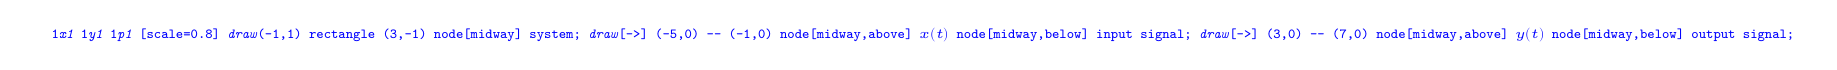
\begin{tikzpicture}[scale=0.8]
		\draw (-1,1) rectangle (3,-1) node[midway] {system};

		\draw[->] (-5,0) -- (-1,0) node[midway,above] {$x(t)$} node[midway,below] {input signal};
		\draw[->] (3,0) -- (7,0) node[midway,above] {$y(t)$} node[midway,below] {output signal};
	\end{tikzpicture}

	\subsection{Περιοδικά σήματα}
	Αν \( \exists T \in \mathbb R : \forall t \in \mathbb R \quad x(t)=x(t+T) \)
	τότε \( x(t) \) \textbf{περιοδικό σήμα} με περίοδο \( T \).

	Ή θα είναι 0, ή θα συνεχιστεί για πάντα.

	\[
	\int_{-\sfrac{T}{2}}^{\sfrac{T}{2}} x(t) \dif t =
	\int_{t_0-\sfrac{T}{2}}^{t_0+\sfrac{T}{2}} x(t) \dif t\ \forall t
	\]

	Η σύνθεση μιας συνάρτησης με μια περιοδική συνάρτηση είναι περιοδική;
	\subparagraph{Απόδ.}
		Έστω \(g\) μία περιοδική συνάρτηση:
		\begin{align*}
		\big(f\circ g\big)(x) &= f\left(g(x)\right) = f \left( g(x+T) \right) =
		\\ &= \big(f\circ g\big)(x+T)
		\end{align*}

	\subsection{Συμμετρίες}
	\begin{itemize}
	    \item Αν \( x(t) = x(-t) \ \forall t \) τότε η \( x(t) \) λέγεται \textbf{άρτια συνάρτηση} (even function).

	    \item Αν \( x(t) = -x(t) \ \forall t \) τότε η \( x(t) \) λέγεται \textbf{περιττή συνάρτηση} (odd function).
	\end{itemize}

	\paragraph{}
	Υποστηρίζω ότι κάθε συνάρτηση μπορεί να γραφεί σαν άθροισμα μιας άρτιας και μιας περιττής:

	\( \forall x(t) \quad \exists\ x_0(t), x_e(t): x(t) = x_e(t)+x_0(t) \)
	\subparagraph{Απόδ.}
	\begin{align*}
		x_e(t) &= \frac{x(t)+x(-t)}{2} \\
		x_o(t) &= \frac{x(t)-x(-t)}{2}.
	\end{align*}

	\paragraph{}
	\begin{align*}
		x{\underbrace{_e}_{\mathclap{\text{άρτια}}}}y_e &= z_e\\
		x_oy_o &=z_e \\
		x_ey_0 &=z_0 \\
		\int_{-A}^A x_0(t)\dif t &= 0 \\
		\int_{-\infty}^\infty x_0(t)\dif t &= ? \text{ (εξαρτάται)} \\
		\lim_{A\to \infty} \int_{-A}^A x_0(t)\dif t &= 0 \quad \text{(principal Cauchy value)}
	\end{align*}

	\subsection{Χαρακτηριστικά σήματα}
	\begin{enumpar}
		\item \textbf{Εκθετικό σήμα}
		\[
		x(t) = ce^{at}\quad a \in \mathbb R \quad c > 0
		\]
		\begin{tikzpicture}
		\draw[->,gray] (0,0) -- (0,4);
		\draw[->,gray] (-2,0) -- (4,0) node[below right] {$t$};

		\draw (1,3) node {$c > 0$};

		\draw[xscale=3,domain=-0.7:1.3,smooth,variable=\x,blue] plot ({\x},{exp(\x)});
		\draw[xscale=3,domain=1.3:-1.2,dashed,smooth,variable=\x,blue] plot ({\x},{exp(-\x)});
		\draw (4,1) node[anchor=north east,blue] {$a < 0$};
		\draw (4.5,3) node[anchor=north east,blue] {$a > 0$};
		\end{tikzpicture}
		\[
		x(t) = ce^{(\sigma t+j\omega)t} = ce^{\sigma t}e^{j\omega t}
		= ce^{\sigma t} \left[
		\cos(\omega t)+j\sin(\omega t)
		\right]
		\]

		\item \textbf{(Συν)ημιτονοειδή σήματα}
		\[
		x(t) = A \cos(\omega t\pm \phi)
		= a \mathrm{Re} \left\lbrace e^{j(\omega t +\phi)} \right\rbrace
		= A \frac{e^{j(\omega t \pm \phi)} + e^{-j(\omega t\pm \phi)}}{2}
		\]
		\begin{tikzpicture}[scale=1.3]
		\draw[->,gray] (0,-2) -- (0,2);
		\draw[->,gray] (-2,0) -- (4,0) node[below right] {$t$};


		\draw[scale=1,domain=0:4,samples=200,smooth,variable=\x,blue,thick] plot ({\x},{sin((\x r)*20)*exp(-\x)});
		\end{tikzpicture}

		\item \textbf{Δέλτα Dirac} \( \delta(t) \)

		
\begin{tikzpicture}[scale=1.2]
		\draw[->,gray] (0,-2) -- (0,2) node[black,below right] {$\delta(t)$};
		\draw[->,gray] (-1,0) -- (1,0) node[below right] {$t$};
		\draw (0,0) node[below left] {$0$};

		\draw[very thick,blue,->] (0,0) -- (0,1);
		\end{tikzpicture}
		
\begin{tikzpicture}[scale=1.2]
		\filldraw[fill=green!20] (-0.5,0) rectangle (0.5,1) node[above right] {$\sfrac{1}{T}$}
			node[midway,right] {$1$};

		\draw[->,gray] (0,-2) -- (0,2);
		\draw[->,gray] (-1.5,0) -- (2,0);

		\draw (current bounding box.east) node[above] {$\lim_{T\to0} P_T(t)=\delta(t)$};
		\end{tikzpicture}
		\begin{tikzpicture}[scale=1.2]
		\filldraw[scale=1,domain=-2:2,samples=200,smooth,variable=\x,fill=green!20]
			plot ({\x},{exp(-\x*\x)})
			node[above right] {$G_\sigma(t) = \frac{1}{\sqrt{2\pi}\sigma}e^{-\frac{x^2}{\sigma^2}} $}
			node[midway,above left] {$1$};

		\draw[->,gray] (0,-2) -- (0,2);
		\draw[->,gray] (-2,0) -- (2,0);

		\draw[<->,gray] (0.7,{exp(-pow(0.7,2))}) -- (-0.7,{exp(-pow(0.7,2))})
			node[above left] {$\sigma$};

		\draw (current bounding box.east) node[below left] {$\lim_{T\to0} G_\sigma(t)=\delta(t)$};
		\end{tikzpicture}
	    \paragraph{Ορ.}
	    \[
	    \int_{-\infty}^\infty f(t) \delta(t) \dif t = f(0)\ \forall f(t)
	    \]
	    \paragraph{}
	    \begin{align*}
	    \int_{-\infty}^\infty \delta(t)\dif t &=1 \\
	    \int_{-\infty}^\infty f(t)\delta(t-\tau) \dif t &= f(\tau) \\
	    \Aboxed{\int_{-\infty}^\infty f(\tau) \delta(t-\tau)\dif \tau &= f(t)} \\
	    \int_{-\infty}^\infty f(t)\delta(t-\tau)\dif \tau &= f(t)
	    \end{align*}

	    \begin{tikzpicture}[scale=2.5]
	    	\draw[->] (-0.5,0) -- (2,0) node[below] {$t$};
	    	\draw[->] (0,-0.2) -- (0,2);

	    	\draw [blue, very thick, mark position=0.7(c)]
	    	plot [smooth, tension=0.5, domain=-0.5:2, samples=9]
	    	(\x,{1+rand/2})
	    	node[below,right] {$f(t)$}
	    	;

	    	\draw[->,very thick] (c |- {(0,0)}) node[below] {$\tau$} -- (c);
	    	\filldraw (c) circle(.5pt);

	    	\draw[->] (-0.5,-3) -- (2,-3);
	    	\draw[->] (0,-3.2) -- (0,-1);

	    	\draw[->,very thick] let \p1=(c) in (c |- {(0,-3)}) node[below] {$\tau$}
	    	--  (\x1,-3cm+\y1) node[above] {$f(t)\delta(t-\tau)$};
	    	\filldraw (c) circle(.5pt);
	    \end{tikzpicture}

	    \paragraph[Ιδιότητες της δ(τ)]{Ιδιότητες της \( \delta(t) \)}
	    \begin{enumerate}
	    	\item \textbf{Κλιμάκωση}
	    	\[
	    	a \in \mathbb R: \delta(at) = \frac{1}{|a|}\delta(t)
	    	\]
	    	\subparagraph{Απόδ.}
	    	\[
	    	\underbrace{\int_{-\infty}^\infty \phi(t)\boxed{\delta(at)}\dif t}_{\mathclap{\begin{matrix}
	    			at=\xi\\\dif t = \frac{\dif \xi}{a}
	    			\end{matrix}}}
	    =
	    	\int_{-\infty_{(a)}}^{\infty_{(a)}} \phi\left( \frac{\xi}{a} \right) \delta(\xi)\frac{\dif \xi}{a}
	    	= \frac{1}{|a|}\int_{-\infty}^\infty \frac{\phi\left(\frac{\xi}{a} \right)}{|a|}\delta(\xi)\dif\xi = \frac{\phi(0)}{|a|}
	    	= \int_{-\infty}^\infty \phi(t)\boxed{\frac{\delta(t)}{|a|}}\dif t
	    	\]
	    	\item \(
	    	f(t)\delta(t)=f(0)\delta(t)
	    	\)
	    	\item \(
	    	f(t)\delta(t-\xi)=f(g)\delta(t-\xi)
	    	\)
    	\end{enumerate}
	\end{enumpar}

	\paragraph{}
	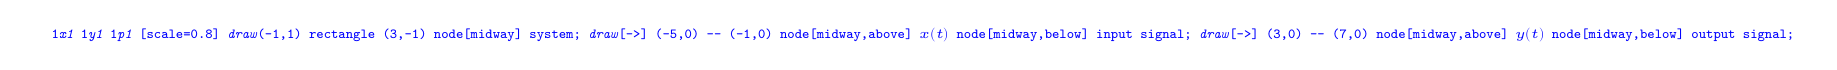
\begin{tikzpicture}[scale=0.8]
	\draw (-1,1) rectangle (3,-1) node[midway] {system};

	\draw[->] (-5,0) -- (-1,0) node[midway,above] {$x(t)$} node[midway,below] {input signal};
	\draw[->] (3,0) -- (7,0) node[midway,above] {$y(t)$} node[midway,below] {output signal};
	\end{tikzpicture}
	\begin{gather*}
		y(t) = \mathscr{L}\left\lbrace x(t) \right\rbrace \\
		\forall x_1(t)\ x_n(t)\\
		y_1(t) = \mathscr{L}\left\lbrace x_1(t) \right\rbrace \\
		y_2(t) = \mathscr{L}\left\lbrace x_2(t) \right\rbrace
	\end{gather*}

	Για const \( a_1, a_2 \in \mathbb R  \)
	\begin{align*}
	x(t) &= a_1x_1(t)+a_2x_2(t) \\
	y(t) &= \mathscr{L}\left\lbrace x(t) \right\rbrace \\
	\intertext{ανν}
	y(t) = a_1y_1(t)+a_2y_2(t) \\
	\intertext{τότε}
	\mathscr{L}: \text{ γραμμικό σύστημα}
	\end{align*}

	\begin{itemize}
		\item \(g(t) = \mathscr{L}\left\lbrace x(t) \right\rbrace\)

		\( x'(t)=x(t-\tau) \)

		ανν \( y'(t) = \mathscr{L} \left\lbrace x'(t) \right\rbrace
		= \mathscr{L} \left\lbrace x(t-\tau)^2 \right\rbrace = y(t-\tau)
		 \)

		 τότε το σύστημα \( \mathscr L \) είναι αμετάβλητο κατά τη μετατόπιση.

	\end{itemize}

	\paragraph{}

    
\begin{tikzpicture}[scale=0.8]
    \draw (-1,-1) rectangle (3,1) node[above right] {$\mathscr L\left\lbrace\right\rbrace$} node[midway] {γραμμικό \& ΑΚΜ};

    \draw[->] (-5,0) -- (-1,0) node[midway,above] {$\delta(t)$} node[midway,below] {input signal};
    \draw[->] (3,0) -- (14,0) node[midway,above] {$\mathrm h(t)$}
	    node[midway,below] {κρουστική απόκριση (impulse response)};
    \end{tikzpicture}

    Υποστηρίζω ότι ένα γραμμικό \& ΑΚΜ σύστημα περιγράφεται πλήρως από την κρουστική
    απόκριση \( h(t) \).
    \subparagraph{Απόδ.} Από παραπάνω, γνωρίζουμε ότι
    \(
    x(t) = \int_{-\infty}^\infty x(t)\delta(t-\tau)\dif \tau
    \)
    \begin{align*}
    y(t) &= \mathscr L \left\lbrace x(t) \right\rbrace =
    \mathscr L \left\lbrace \int_{-\infty}^{\infty} x(t)\delta(t-\tau) \dif \tau
     \right\rbrace
     \\ & \overset{\text{linearity}}{=} \int_{-\infty}^{\infty} \mathscr L
     \left\lbrace x(t)\delta(t-\tau) \right\rbrace \dif\tau
     \\ &= \int_{-\infty}^{\infty} x(\tau) \mathscr L \left\lbrace
     \delta(t-\tau)
      \right\rbrace \dif \tau
      \\ & \underset{\underbrace{\text{TSI}}_{\text{Time shift invariant}}}{\overset{\text{ΑΚΜ}}{=}}
       \int_{-\infty}^{\infty} x(\tau) h(t-\tau)\dif \tau
       \\ y(t) &= \int_{-\infty}^{\infty}
        x(\tau)
        \underbrace{h(t-\tau)}_{\mathclap{\text{linear time-shift invariant}}}
        \dif\tau
    \end{align*}

    \paragraph{}

    \begin{itemize}
    	\item \( \delta(t)=\delta(-t) \) άρτια συνάρτηση
    	\item \( \delta^{(n)}(t) = \od[n]{}{t}\delta(t) \), για την οποία
    αποδεικνύεται ότι:
        \[
            \int_{-\infty}^{\infty} \delta^{(n)}(t)\phi(t)\dif t
            = (-1)^n\left.\phi^{(n)}(t)\right|_{t=0}
        \]
    \end{itemize}

    \subsection{Χρήσιμες Συναρτήσεις}

    \subsubsection{Βηματική Συνάρτηση (Unit Step Function)}
    \[
    \mathrm u(t) = \begin{cases}
    1 \quad & t > 0 \\
    0 \quad & t < 0
    \end{cases}
    \]
    \[
    \int_{-\infty}^{\infty} \mathrm u(t)\phi(t)\dif t =
    \mathscr N_{\mathrm u}\left\lbrace \phi(t) \right\rbrace =
    \underbrace{ \int_0^\infty \phi(t)\dif t}_{\mathclap{\text{number}}}
    \]
    
\begin{tikzpicture}
    \begin{axis}[%
    xlabel=$t$
    ,ylabel=$\mathrm u(t)$
    ,axis lines = center
    ,ymax=1.5
    ,ytick={0,1}
    ,xtick={0,1}
    ]
    \addplot+[const plot, no marks,ultra thick] coordinates {(-4,0) (0,1) (4,1)};
    %\addplot+[const plot, no marks, thick] coordinates {(0,0) (1,0.25) (2,0.4) (3,0.5) (4,1) (4.49,1)} node[below=1.15cm,pos=.76,black] {$F_y$};
    \end{axis}
    \end{tikzpicture}

    \begin{align*}
    \delta(t) &= \od{}{t} \mathrm u(t)\\
    \mathrm u(t) &= \int_{-\infty}^t \delta(\tau)\dif\tau =
    \int_0^\infty \delta(t-\xi)\dif\xi
    \end{align*}

    \subsubsection{Ράμπα}
    \[
    \mathrm r(t) = \int_{-\infty}^t \mathrm u(\tau)\dif\tau =
    \begin{cases}
    t \quad & t \geq0 \\
    0 \quad & \text{else}
    \end{cases} = t\mathrm u(t)
    \]

    
\begin{tikzpicture}
    	\draw[->] (0,-0.5) -- (0,4) node[right] {$\mathrm r(t)$};
    	\draw[->] (-2,0) -- (4,0) node[below] {$t$};

    	\draw (0,0) node[below right] {$0$};

    	\draw[very thick,blue] (-2,0) -- (0,0) -- (3.5,3.5);
    \end{tikzpicture}

    \[
    \mathrm u(t) =\od{}{t} \mathrm r(t)
    \]

    \subsubsection{Ορθογωνικός παλμός (Rectangular Pulse function)}
    \[
    \mathrm p_a(t) = \begin{cases}
    1 &\quad |t| < a \\
    0 &\quad |t| > a
    \end{cases}
    \]

    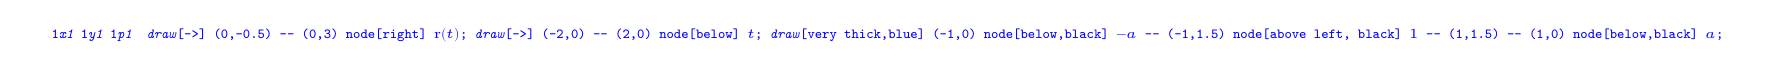
\begin{tikzpicture}
    \draw[->] (0,-0.5) -- (0,3) node[right] {$\mathrm r(t)$};
    \draw[->] (-2,0) -- (2,0) node[below] {$t$};

    \draw[very thick,blue]
	    (-1,0) node[below,black] {$-a$} --
	    (-1,1.5) node[above left, black] {$1$} --
	    (1,1.5) --
	    (1,0) node[below,black] {$a$};
    \end{tikzpicture}

    \subparagraph{}

    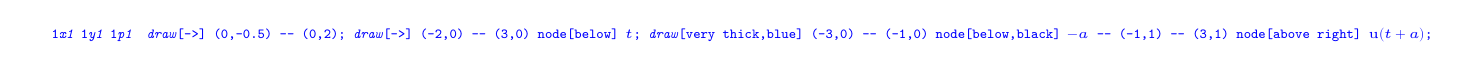
\begin{tikzpicture}
    \draw[->] (0,-0.5) -- (0,2);
    \draw[->] (-2,0) -- (3,0) node[below] {$t$};

    \draw[very thick,blue]
    (-3,0) --
    (-1,0) node[below,black] {$-a$} --
    (-1,1) --
    (3,1) node[above right] {$\mathrm u(t+a)$};
    \end{tikzpicture}
    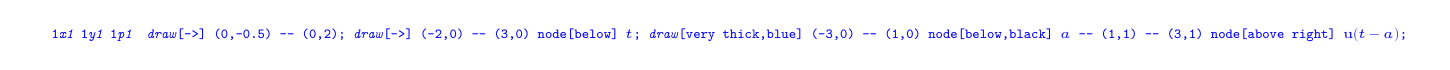
\begin{tikzpicture}
    \draw[->] (0,-0.5) -- (0,2);
    \draw[->] (-2,0) -- (3,0) node[below] {$t$};

    \draw[very thick,blue]
    (-3,0) --
    (1,0) node[below,black] {$a$} --
    (1,1) --
    (3,1) node[above right] {$\mathrm u(t-a)$};
    \end{tikzpicture}

    \begin{align*}
    \mathrm p_a(t) =& \mathrm u(t+a) - \mathrm u(t-a) \\
    \od{}{t} \mathrm p_a(t) =& \delta(t+a)-\delta(t-a)
    \end{align*}

    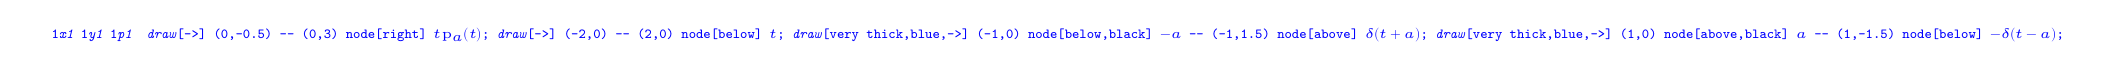
\begin{tikzpicture}
    \draw[->] (0,-0.5) -- (0,3) node[right] {$\od{}{t}\mathrm p_a(t)$};
    \draw[->] (-2,0) -- (2,0) node[below] {$t$};

    \draw[very thick,blue,->]
    (-1,0) node[below,black] {$-a$} --
    (-1,1.5) node[above] {$\delta(t+a)$};

    \draw[very thick,blue,->]
    (1,0) node[above,black] {$a$} --
    (1,-1.5) node[below] {$-\delta(t-a)$};
    \end{tikzpicture}

    \subsubsection{Τριγωνικός Παλμός (Triangular Pulse function)}
    \[
    \mathrm p_{\mathrm{tr},a} = \begin{cases}
    1-\frac{|t|}{a} &\quad |t|<a \\
    0 &\quad |t|>a
    \end{cases}
    \]
    
\begin{tikzpicture}[scale=1.2]
    \draw[->] (0,-0.5) -- (0,2) node[right] {$\mathrm p_{\mathrm{tr},a}(t)$};
    \draw[->] (-2,0) -- (2,0) node[below] {$t$};

    \draw[very thick,blue]
    (-2,0) --
    (-1,0) node[below,black] {$-a$} --
    (0,1.5) node[above left, black] {$1$} --
    (1,0) node[below,black] {$a$} --
    (2,0);
    \end{tikzpicture}
    \[
    p_{\mathrm{tr},a}(t) = \frac{1}{a} \left[
        \mathrm r(t+a) + \mathrm r(t-a) - 2\mathrm r(t)
    \right]
    \]
    
\begin{tikzpicture}[scale=0.7]
    	\draw[gray] (-4,0) -- (4,0);
    	\draw[gray] (0,-4) -- (0,4);

    	\draw[dashed] (-2,0) -- (1,3);
    	\draw[dashed] (2,0) -- (4,2);
    	\draw[dashed] (0,0) -- (2,-4);

    	\draw[blue,opacity=.3,very thick] (-4,0) -- (-2,0) -- (0,2) -- (2,0) -- (4,0);
    \end{tikzpicture}

    \subsection{Χαρακτηριστικά Μεγέθη}
    \begin{enumpar}
    	\item \textbf{Μέση τιμή (Mean Value)}
    	\[
    	\overline{x(t)} = \frac{1}{t_2-t_1} \int_{t_1}^{t_2}x(t)\dif t
    	\]

    	Αν περιοδική τότε \begin{align*}
    	\bar x(t) &= \frac{1}{T} \int_0^T x(t)\dif t \\
    	&= \frac{1}{T} \int_{t_0}^{t_0+T} x(t)\dif t
    	\end{align*}
    	\item \textbf{Ενεργός τιμή (Root Mean Square Value)}
    	\[
    	\overline{\overline{x(t)}} = \left[
    	    \frac{1}{t_2-t_1}\int_{t_1}^{t_2} x^2(t)\dif t
    	\right]^{\sfrac{1}{2}}
    	\]
    	Αν ημιτονοειδές σήμα \(\bar{\bar{x}}(t) = \frac{x_{\max}}{\sqrt{2}}
    	\)

    	\item \textbf{Ενέργεια - Ισχύς}
    	\begin{itemize}
    		\item Στιγμιαία ισχύς (Instant power)
    		\[
    		p(t) = x^2(t)
    		\]
    		\item Μέση ισχύς (Mean power)
    		\[
    		\overline{p(t)} = \frac{1}{t_2-t_1}\int_{t_1}^{t_2}x^2(t)\dif t
    		= \left( \overline{\overline{x(t)}} \right)^2
    		\]
    		\item Ενέργεια (Energy)
    		\[
    		W = \int_{t_1}^{t_2} p(t) \dif t =
    		\int_{t_1}^{t_2} x^2(t)\dif t = (t_2-t_1)\left(
    		\overline{\overline{x(t)}}
    		\right)^2
    		\]
    	\end{itemize}

    	\textbf{Σήματα} \( \begin{dcases}
    	\text{\textbf{Σήμα ενέργειας} αν} \lim_{T\to \infty}W< \infty
    	\\ \\
    	\text{\textbf{Σήμα ισχύος} αν} \lim_{T\to \infty}\overline{p(t)}>0
	    \\ \text{Υπάρχουν και σήματα που δεν είναι ούτε ενέργειας, ούτε ισχύος.}
    	\end{dcases}
    	\)
    \end{enumpar}

    \subsection{Συνέλιξη}
    \[ x(t) = \int_{-\infty}^{\infty}x(t)\delta(t-\tau)d\tau \]
    
\begin{tikzpicture}[scale=0.7]
    \draw (-1,-1) rectangle (3,1) node[above right] {$\mathscr L\left\lbrace\right\rbrace$} node[midway,align=center]
    {γραμμικό\\ \& \\ ΑΚΜ};

    \draw[->] (-5,0) -- (-1,0) node[midway,above] {$\delta(t)$} node[midway,below] {input signal};
    \draw[->] (3,0) -- (9,0) node[midway,above] {$\mathrm h(t)$}
    node[midway,below,align=center] {κρουστική απόκριση\\ (impulse response)};
    \end{tikzpicture}
    \[ h(t)=\mathscr L\left\lbrace \delta(t) \right\rbrace \]
    \[ y(t) = \int_{-\infty}^{\infty} x(\tau)h(t-\tau)\dif\tau
    = \underbrace{x(t)}_{\mathclap{\text{είσοδος}}}
    \overset{\substack{\text{συνέλιξη}\\\uparrow}}{*}
    \underbrace{h(t) }_{\mathclap{\text{κρουστική απόκριση}}}\]

    \paragraph{Συνέλιξη - Convolution}
    \[
    z(t)=x(t)*y(t)=\int_{-\infty}^{\infty} x(\tau)y(t-\tau)\dif\tau
    \]

    \paragraph{}
    \begin{itemize}
    	\item \(x(t)*y(t)=y(t)*x(t)\) \textbf{Αντιμεταθετική}
    	\subparagraph{}
    	\[
    	\int_{-\infty}^{\infty} x(\tau)y(t-\tau)\dif\tau
    	= \int_{-\infty}^{\infty} x(t-\lambda)y(\lambda)[-\dif\lambda]
    	= \int_{-\infty}^{\infty} y(\lambda)x(t-\lambda)\dif\lambda
    	= y(t)*x(t)
    	\]
    	\item \( x_1(t)*\left[x_2(t)*x_3(t)\right] =
    	\left[x_1(t)*x_2(t)\right]*x_3(t) \) \textbf{Προσεταιριστική}
    \end{itemize}

    \paragraph{Παρ.}
    \begin{align*}
    f_1(t) &= 2(1-t)\left[ \mathrm u(t)-u(t-1) \right] \\
    f_2(t) &= \mathrm u(t) - \mathrm u(t-\tau)
    \end{align*}

    \subparagraph{Γραφική μέθοδος υπολογισμού συνέλιξης}
    \hspace{0pt}
    \\

    
\begin{tikzpicture}[every node/.style={black}]
	    \draw (0,3) -- (0,-3.5);

    	\draw (-3,0) -- (3,0) node[below] {$\tau$};
    	\draw (-3,-3) -- (3,-3) node[below] {$\tau$};

    	\draw[very thick,blue] (0,2)
    	node[left] {$2$}
    	node[above right,black] {$f_1(\tau)$}
    	-- (1,0) node[below] {$1$};

    	\draw[very thick,blue] (0,-2)
    	node[left] {$1$}
    	node[above right,black] {$f_2(\tau)$}
    	-- (2,-2) -- (2,-3) node[below] {$2$};
    	\draw[dashed] (1,-3) node[below] {$1$} -- (1,-2);
    \end{tikzpicture}


    
\begin{tikzpicture}[every node/.style={black}]
    	\draw (-3,0) -- (3,0) node[below] {$\tau$};
    	\draw[->] (0,-1) -- (0,2);

    	\draw[very thick,blue]
    	(-2,0) node[below] {$-2$}
    	-- (-2,1)
    	-- (0,1) node[above right,blue] {$f_2(-\tau)$}
    	-- (0,0) node[below left] {$0$}
    	;
    \end{tikzpicture}


    
\begin{tikzpicture}[every node/.style={black}]
    \draw (-3,0) -- (3,0) node[below] {$\tau$};
    \draw[->] (0,-1) -- (0,2);

    \draw[very thick,blue]
    (-0.8,0)
    -- (-0.8,1)
    -- (1.2,1) node[above right,blue] {$f_2(t-\tau)$}
    -- (1.2,0)
    ;

    \draw[<->] (0,1.4) -- (1.2,1.4) node[midway,fill=white,inner sep=2pt] {$t$};
    \end{tikzpicture}

    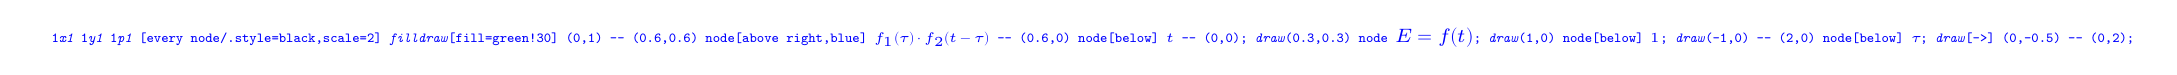
\begin{tikzpicture}[every node/.style={black},scale=2]
    \filldraw[fill=green!30]
    (0,1)
    -- (0.6,0.6)  node[above right,blue] {$f_1(\tau)\cdot f_2(t-\tau)$}
    -- (0.6,0) node[below] {$t$}
    -- (0,0);

    \draw (0.3,0.3) node {\scriptsize $E=f(t)$};
    \draw(1,0) node[below] {$1$};

    \draw (-1,0) -- (2,0) node[below] {$\tau$};
    \draw[->] (0,-0.5) -- (0,2);
    \end{tikzpicture}

    \begin{itemize}
    	\item \(t<0\)
    	
\begin{tikzpicture}[baseline={([yshift=-.8ex]current bounding box.center)}]
    		\draw (-2,0) -- (2,0);
    		\draw (0,-0.2) -- (0,1.5);
    		\draw[very thick,blue] (0,1) -- (1,0);

    		\draw (-2,-2) -- (2,-2);
    		\draw (0,-2.2) -- (0,-0.5);
    		\draw[very thick,blue] (-1.8,-2) -- (-1.8,-1.2) -- (-0.3,-1.2) -- (-0.3,-2);
    	\end{tikzpicture}
    	\(f(t) = 0\)

    	\item \(0<t<1\)
    	\begin{tikzpicture}[baseline={([yshift=-.8ex]current bounding box.center)}]
    	\fill[green!30] (0,1) -- (0.7,0.3) -- (0.7,0) -- (0,0);
    	\draw[gray] (0.7,-0.2) node[below] {$t$} -- (0.7,0) -- (0.7,0.3);

    	\draw (-2,0) -- (2,0);
    	\draw (0,-0.2) -- (0,1.5);
    	\draw[very thick,blue] (0,1) -- (1,0);
    	\draw (1,0) node[below] {$1$};

    	\draw (-2,-2) -- (2,-2);
    	\draw (0,-2.2) -- (0,-0.5);
    	\draw[very thick,blue] (-0.8,-2) -- (-0.8,-1.2) -- (0.7,-1.2) -- (0.7,-2);
    	\draw(0.7,-2) node[below]{$t$};
    	\end{tikzpicture}
    	\(f(t) =  \frac{1}{2}(2+2-2t)t=(2-t)t \)

    	\item \(1<t<2\)
    	\begin{tikzpicture}[baseline={([yshift=-.8ex]current bounding box.center)}]
    	\fill[green!30] (0,1) -- (1,0) -- (0,0);

    	\draw (-2,0) -- (2,0);
    	\draw (0,-0.2) -- (0,1.5);
    	\draw[very thick,blue] (0,1) -- (1,0);
    	\draw (1,0) node[below] {$1$};

    	\draw (-2,-2) -- (2,-2);
    	\draw (0,-2.2) -- (0,-0.5);
    	\draw[very thick,blue] (-0.3,-2) -- (-0.3,-1.2) -- (1.2,-1.2) -- (1.2,-2);
    	\draw(1.2,-2) node[below]{$t$};
    	\end{tikzpicture}
    	\(f(t) =  1 \)

    	\item \(2<t<3\)
    	\begin{tikzpicture}[baseline={([yshift=-.8ex]current bounding box.center)}]
    	\fill[green!30] (0.5,0.5) -- (1,0) -- (0.5,0);
    	\draw[gray] (0.5,0) -- (0.5,0.5);

    	\draw (-2,0) -- (2,0);
    	\draw (0,-0.2) -- (0,1.5);
    	\draw[very thick,blue] (0,1) -- (1,0);
    	\draw (1,0) node[below] {$1$};

    	\draw (-2,-2) -- (2.4,-2);
    	\draw (0,-2.2) -- (0,-0.5);
    	\draw[very thick,blue] (0.5,-2) -- (0.5,-1.2) -- (2,-1.2) -- (2,-2);
    	\draw(2,-2) node[below]{$t$};
    	\end{tikzpicture}
    	\(f(t) = \frac{(t-1)\cdot2\cdot\left(1-(t-2)\right)}{2}=(t-1)(3-t) \)

    	\item \(t>3\)
    	
\begin{tikzpicture}[baseline={([yshift=-.8ex]current bounding box.center)}]
    	\draw (-2,0) -- (2,0);
    	\draw (0,-0.2) -- (0,1.5);
    	\draw[very thick,blue] (0,1) -- (1,0);
    	\draw (1,0) node[below] {$1$};

    	\draw (-2,-2) -- (3.4,-2);
    	\draw (0,-2.2) -- (0,-0.5);
    	\draw[very thick,blue] (1.2,-2) -- (1.2,-1.2) -- (2.7,-1.2) -- (2.7,-2);
    	\end{tikzpicture}
    	\(f(t) = 0 \)
    \end{itemize}
    \begin{tikzpicture}[scale=1.3]
    	\draw[->] (0,-0.2) -- (0,2);
    	\draw (-1,0) -- (4,0) node[below] {$t$};

    	\draw[ultra thick,red!80!green]
    	(-1,0)
    	-- (0,0)
    	plot[domain=0:1] (\x,{(2-\x)*\x})
    	-- (2,1) node[above,midway,black] {$f(t)$}
    	plot[domain=2:3] (\x,{(\x-1)*(3-\x)})
    	-- (4,0)
    	;
    \end{tikzpicture}

    \subparagraph{Αναλυτική μέθοδος}
    \hspace{0pt}

    Παρατηρώ ότι: \[
    \int_{-\infty}^{\infty} f(t,\tau) \mathrm u(\tau-\xi)\mathrm u(\phi-\tau)\dif\tau
    = \int_{\xi}^\phi f(t,\tau)\dif\tau\mathrm u(\phi-\xi)
    \]

	{
	\setlength{\mathindent}{-10cm}
    \begin{align*}
    f(t) &= \int_{-\infty}^{\infty}
    \underbrace{2(1-\tau)}_{\mathclap{x(\tau)}}\left[\mathrm u(\tau)-\mathrm u(\tau+1) \right]\left[
    \mathrm u(t-\tau)-\mathrm u(t-\tau-2)
    \right] \dif\tau \\
    &= \int_{-\infty}^{\infty} x(\tau) \left[
    \mathrm u(\tau)\mathrm u(t-\tau)-\mathrm u(\tau-1)\mathrm u(t-\tau)
    -\mathrm u(\tau)\mathrm u(t-\tau-2)+\mathrm u(\tau-1)\mathrm u(t-\tau-2)
    \right]\dif\tau \\
    &= \int_0^t x(\tau)\dif\tau\mathrm u(t)
    -\int_1^x x(\tau)\dif\tau \mathrm u(t-1)
    -\int_0^{t-2}x(\tau)\dif\tau \mathrm u(t-2)
    +\int_1^{t-2}x(\tau)\dif\tau\mathrm u(t-3)
    \\ &=
    (2t-t^2)\mathrm u(t) - \left[2t-t^2-1\right]\mathrm u(t-1)
    - \left[ 2(t-2)-(t-2)^2 \right] \mathrm u(t-2)+
    \left[
    2(t-2)-(t-2)^2-1
    \right] \mathrm u(t-3)
    \end{align*}
	}

    \paragraph{Ex}
    \begin{align*}
    f_1(t) &= e^t\mathrm u(-t) \\
    f_2(t) &= \mathrm u(-t+2) \\
    f &= f_1*f_2
    \end{align*}
    \begin{align*}
    f &= \int_{-\infty}^{\infty}  e^\tau \mathrm u(-\tau)
    \mathrm u\left( -(t-\tau)+2 \right)\dif\tau
    \\&= \int_{-\infty}^{\infty} e^\tau \mathrm u(-\tau)
    \mathrm u(\tau-t+2)\dif\tau
    \\&= \int_{t-2}^0 e^\tau\dif\tau\mathrm u(t-2)
    \\&= \left. e^\tau \right|_{t-2}^0\mathrm u(2-t)
    \\&=\left[ 1-e^{t-2} \right]\mathrm u(2-t)
    \end{align*}

	\paragraph{}
	\begin{align*}
	\int_{-\infty}^{\infty} f(t,\tau)\mathrm u(\tau-\xi)\mathrm u(\phi-\tau)\dif\tau
	=\int_\xi^\phi f(t,\tau)\dif \tau \mathrm u(\phi-\xi)
	\end{align*}

	\paragraph{Ex.} \hspace{0pt}\\


	
\begin{tikzpicture}
		\draw (-3,0) -- (3,0);
		\draw (0,-2) -- (0,2);

		\draw[very thick,blue,->] (0,0) node[below left,black] {$0$}
		-- (0,1) -- (-1,1) node[above,midway] {$\mathrm u(-\tau)$};

		\draw[very thick,blue,->] (-1.4,0) node[below,black] {$t+2$}
		-- (-1.4,0.6) -- (-2.6,0.6);

		\draw[very thick,blue,->] (1.4,0) node[below,black] {$t+2$}
		-- (1.4,0.6) -- (0.2,0.6);
	\end{tikzpicture}

	
\begin{tikzpicture}[scale=1.7]
		\draw (-4,0) -- (-2,0);
		\draw[very thick,blue,->] (-3.2,0) node[below,black] {$t+2$}
		-- (-3.2,0.5) -- (-4,0.5) node[above,midway] {$\mathrm u(t+2-\tau)$};
		\draw[very thick,blue,->] (-2.4,0) node[below,black] {$0$}
		-- (-2.4,1.1) -- (-3.2,1.1) node[above,midway] {$\mathrm u(-\tau)$};
		\draw (-3,-0.7) node {$\overbrace{t+2<0}$};

		\draw (-1,0) -- (1,0);
		\draw[very thick,blue,->] (0.5,0) node[below,black] {$t+2$}
		-- (0.5,0.5) node[right] {$\mathrm u(t+2-\tau)$} -- (-0.5,0.5);
		\draw[very thick,blue,->] (0,0) node[below,black] {$0$}
		-- (0,1.1) -- (-1,1.1) node[above,midway] {$\mathrm u(-\tau)$};
		\draw (0,-0.7) node {$\overbrace{t+2\geq0}$};
	\end{tikzpicture}

	\begin{align*}
	x(t) &= e^t\mathrm u(-t) \\
	y(t) &= \mathrm u(t+2) \\
	z(t) &= x(t)*y(t) = \int_{-\infty}^{\infty} e^\tau \mathrm u(-\tau)
	\mathrm u \left[(t-\tau)+2\right]\dif\tau
	= \int_{-\infty}^{\infty} e^\tau \mathrm u(-\tau)\mathrm u(t+2-\tau)\dif\tau
	\\ &= \int_{-\infty}^{\infty} e^\tau\left[1-\mathrm u(t)\right]
	\mathrm u(t+2-\tau)\dif \tau \\ &=
	\int_{-\infty}^{\infty} e^\tau \mathrm u(t+2-\tau)\dif\tau-
	\int_{-\infty}^{\infty} e^\tau \mathrm u(\tau)u(t+2-\tau)\dif\tau
	\\ &= \int_{-\infty}^{t+2}e^\tau\dif \tau
	\cancelto{1}{\mathrm u\left(t+2-(-\infty)\right)} - \int_0^{t+2}
	e^\tau\dif\tau \mathrm u(t+2)
	\\ &= e^{t+2}-\left[ e^{t+2}- 1 \right]\mathrm u(t+2)
	\end{align*}

	\paragraph{Ex.}
	\begin{align*}
	x(t) &= e^t\mathrm u(-t) \\
	y(t) &= \mathrm u(t+2)-\mathrm u(t+1) \\
	z(t) &= x(t) * y(t) = \int_{-\infty}^{\infty} x(\tau)y(t-\tau)\dif\tau
	= \int_{-\infty}^{\infty} e^\tau\mathrm u(-\tau)\left[
	\mathrm u(t-\tau+2)-\mathrm u(t-\tau+1)
	\right]\dif\tau
	\\ &= \int_{-\infty}^{\infty} e^\tau
	\mathrm u(-\tau)\mathrm u(t-\tau+2)\dif\tau - \int_{-\infty}^{\infty}
	e^\tau \mathrm u(-\tau)\mathrm u(t-\tau+1)\dif\tau
	\\ &= \int_{-\infty}^{\infty} e^\tau
	\left[ 1-\mathrm u(\tau) \right]\mathrm u(t-\tau+2)\dif\tau -
	\int_{-\infty}^{\infty} e^\tau \left[ 1-\mathrm u(\tau) \right]
	\mathrm u(t-\tau+1)\dif\tau
	\\ &= \int_{-\infty}^{\infty}
	\mathsmaller{e^\tau \mathrm u(t-\tau+2)\dif\tau}
	- \int_{-\infty}^{\infty}
	\mathsmaller{\mathsmaller{
		 e^\tau \mathrm u(\tau) \mathrm u(t-\tau+2)\dif\tau}}
	- \int_{-\infty}^{\infty}
	\mathsmaller{\mathsmaller{ e^\tau \mathrm u(t-\tau+1)\dif\tau}}
	+ \int_{-\infty}^{\infty}\mathsmaller{\mathsmaller{
		 e^\tau \mathrm u(\tau)\mathrm u(t-\tau+1)\dif\tau}}
	\\ &= \int_{-\infty}^{t+1} e^\tau\dif\tau - \int_{-\infty}^{t+1}e^\tau\dif\tau
	- \int_0^{t+2}e^\tau\dif\tau\mathrm u(t+2)
	+ \int_0^{t+1}e^\tau\dif\tau \mathrm u(t+1)
	\\ &= \int_{t+1}^{t+2}e^\tau\dif\tau
	-\left[ e^{t+2}-1 \right]\mathrm u(t+2)
	+\left[ e^{t+1}-1 \right]\mathrm u(t+1)
	\end{align*}

	\vspace{1cm}
	\paragraph{}
	\( \exists h(t) \) ανν LTI
	\begin{align*}
		y(t) &= x(t)*h(t) \\ &=\int_{-\infty}^{\infty} x(\tau)h(t-\tau)\dif\tau
		\\ &= \int_{-\infty}^{\infty} h(\tau)x(t-\tau)\dif\tau
	\end{align*}

	Έστω ότι η \( x(t) = e^{j\omega t} \)
	\begin{align*}
	y(t) &= \int_{-\infty}^{\infty} h(t) e^{j\omega(t-\tau)}\dif\tau
	= e^{j\omega t} \int_{-\infty}^{\infty} h(\tau)e^{-j\omega\tau}\dif\tau
	\\ &= x(t)\underbrace{\int_{-\infty}^{\infty} h(\tau)e^{-j\omega\tau}\dif\tau}_{\mathclap{h(t) \xrightarrow{FT} H(\omega)}}
	\end{align*}

	\begin{align*}
	x(t) &= A_1e^{j\omega_1 t} + A_2e^{j\omega_2 t} \\
	y(t) &= A_1e^{j\omega_1 t}H(\omega_1)+A_2e^{j\omega_2t}H(\omega_2)
	\end{align*}

        \section{Συναρτηστιακοί χώροι}
    Διανυσματικός χώρος \( S \)
    \[
    \bar x,\quad \bar y\quad S
    \]

    \paragraph{Εσωτερικό γινόμενο}
    \[ \left\langle\bar x,\bar y\right\rangle\ \in \mathbb C  \]
    \begin{enumpar}
        \item \( \left\langle\bar x,\bar y\right\rangle
        = \left\langle\bar y,\bar x\right\rangle^* \)
        \item \( c\left\langle\bar x,\bar y\right\rangle
        =\left\langle c\bar x,\bar y\right\rangle \)
        \item \( \left\langle\bar x+\bar y,\bar z\right\rangle
        = \left\langle\bar x,\bar z\right\rangle+\left\langle\bar y,\bar z\right\rangle \)
        \item \( \left\langle\bar x,\bar x\right\rangle \ \geq 0 \) με
        \( \left\langle\bar x,\bar x\right\rangle = 0 \) ανν \( \bar x = \bar 0 \)
    \end{enumpar}

    \paragraph{Νόρμα}
    \[
    \bar x \in S
    \]\[
    ||\bar x|| \geq0
    \]
    \begin{enumpar}
        \item \( ||\bar x|| = 0 \) ανν \( \bar x = \bar 0 \)
        \item \( ||a\bar x|| = |a|||\bar x|| \quad x \in\mathbb C \)
        \item \( ||\bar x+\bar y|| \leq ||\bar x|| + ||\bar y|| \)
    \end{enumpar}
    \paragraph{Μέτρο:} Απόσταση μεταξύ \( \bar x,\bar y \in S \)
    \begin{enumpar}
        \item \( d(\bar x,\bar y)\geq 0 \qquad d(\bar x,\bar y)=0 \)
        ανν \( \bar x = \bar y \)
        \item \( d(\bar x,\bar y) = d(\bar y,\bar x) \)
        \item \( d(\bar x,\bar y) \leq d(\bar x,\bar z) + d(\bar y,\bar z)
        \quad \bar z\in S
         \)

    \end{enumpar}
    
    \paragraph{Συναρτησιακός χώρος}
    \[
    x(t),y(t) \in S =
    \left\lbrace x(t)/x(t):[t_1,t_2]\to\mathbb R  \right\rbrace
    \]
    \begin{gather*}
    \left\langle
    x(t),y(t)
    \right\rangle  = \int_{t_1}^{t_2}x(t)y(t)\dif t\\
    \left\vert\middle\vert x(t)\middle\vert\right\vert =
    \left[ \int_{t_1}^{t_2} x^2(t)\dif t \right]^{\sfrac{1}{2}}\\
    d\left(
    x(t),y(t)
    \right)=\left[
    \int_{t_1}^{t_2} \left[ x(t)-y(t) \right]^2\dif t
    \right]^{\sfrac{1}{2}}
    \end{gather*}
    
    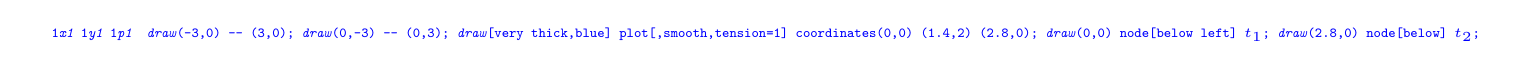
\begin{tikzpicture} %TODO
        \draw (-3,0) -- (3,0);
        \draw (0,-3) -- (0,3);
        
        \draw[very thick,blue] plot[,smooth,tension=1]
        coordinates{(0,0)  (1.4,2)  (2.8,0)};
        
        \draw (0,0) node[below left] {$t_1$};
        \draw (2.8,0) node[below] {$t_2$};
    \end{tikzpicture}
    %TODO Add missing graph
    
    \begin{align*}
    \text{Αν } & \left\langle \phi_1(t),\phi_2(t) \right\rangle
    = 0 \quad \phi_1(t) \perp \phi_2(t) \\
    & \left\langle \phi_1(t),\phi_1(t)\right\rangle = 1 \quad
    \phi_1(t) \text{ κανονική}
    \end{align*}
    
    %TODO Add more missing notes
    
    %TODO Rekanos Graph 11
    
    %TODO Mess starts here
    \paragraph{Τερατοχώρος}
    
    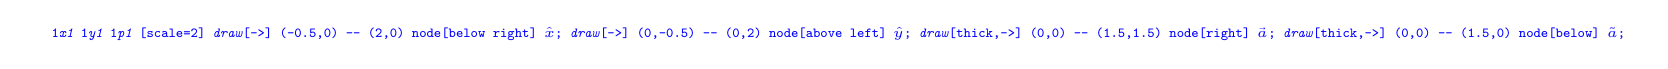
\begin{tikzpicture}[scale=2]
        \draw[->] (-0.5,0) -- (2,0) node[below right] {$\hat x$};
        \draw[->] (0,-0.5) -- (0,2) node[above left] {$\hat y$};
        
        \draw[thick,->] (0,0) -- (1.5,1.5) node[right] {$\vec a$};
        \draw[thick,->] (0,0) -- (1.5,0) node[below] {$\tilde a$};
    \end{tikzpicture}
    
    \( \hat x,\hat y \) όχι εξαρτημένα (συνευθειακά)
    
    Ποια είναι η καλύτερη προσέγγιση για το \(\vec a\) εφ' όσον δεν υπάρχει
    το \( \vec y \);
    
    \( \tilde a \) best γιατί \(\mathrm d(\vec a,\tilde a)\) min.
    
    Άρα:
    \begin{gather*}
        \tilde a = k\hat x \\
        \vec a = a_x\hat x+a_y\hat y\\
        \vec a -\tilde a = (a_x-k)\hat x - a_y\hat y\\
        d(\vec a,\tilde a) = \sqrt{(a_x-k)^2+a_y^2} \\
        \od{}{k}\left( d(\vec a,\tilde a) \right) = \frac{a_x-k}{\cdots}
        = 0 \implies k=a_x = \tilde a \cdot \hat x\\
        \vec a\cdot\hat x = a_x
    \end{gather*}
    
    Η βέλτιστη έκφραση του \( \vec a \) στο δισδιάστατο χώρο είναι το ίδιο το \( \vec a \).
    
    \paragraph{Μη κάθετα διανύσματα}
    
    %TODO There are some shapes here
    
    \begin{gather*}
    \vec a = a_x\hat x+a_y\hat y\\
    \vec a - \tilde a = (a_x-k)\hat x+a_y\hat y\\
    \mathrm d(\vec a,\tilde a)= ||\vec a - \tilde a|| = \sqrt{(\vec a-\tilde a)(\vec a-\tilde a)}
    =\left(
    \left[ (a_x-k)\hat x+a_y\hat y \right]\cdot
    \left[ (a_x-k)\hat x+a_y\hat y \right]
    \right)^{\sfrac{1}{2}}\\
    \left[
    (a_x-k)^2+a_y^2+2(a_x-k)a_y\hat x\cdot\hat y
    \right]^{\sfrac{1}{2}} \\
    \vec a_{\mathrm{best}} = (\vec a \cdot \hat x)\hat x \neq a_x \\
    \boxed{\vec a \cdot \hat x = a_x+a_y\cos\phi\neq a_x}
    \end{gather*}
    
    %TODO There are some shapes here


    \paragraph{Συναρτηστιακός κόσμος}
    \( \phi_n(t) \) παράγουν χώρο με το μηχανισμό:
    \[
    f(t)=\sum_{n=0}^\infty a_n\phi_n(t)\quad t \in \Delta
    \]
    
    \( \phi_n(t) \) ανεξάρτητες μεταξύ τους (βάση απειροδιάστατου χώρου)
    
    \begin{gather*}
    \hat f(t)=\sum_{n=0}^M \underbrace{\hat a_n}_{%
        \mathclap{\neq a_n\text{, επειδή η βάση δεν είναι ορθοκανονική}}
        }\phi_n(t) \text{ βέλτιστη, ώστε η απόσταση με την $f$
        να είναι ελάχιστη}  \\
    \end{gather*}
    
    \begin{align*}
        \overbrace{I^2}^{\mathclap{\text{σφάλμα}}} &=
        \int_\Delta\left[ f(t)-\hat f(t) \right]^2\dif t
        \\ &=
        \int_\Delta \left[
            \sum_{n=0}^{+\infty}a_n\phi_n(t)-\sum_{n=0}^M\hat a_n\phi(t)
        \right]^2\dif t
        \\ &= \int_\Delta f^2(t)\dif t + \int_\Delta \left(
            \sum_{n=0}^M \hat a_n\phi_n(t)
        \right)^2\dif t -2\int_{\Delta}\left[
            f(t)\sum_{n=0}^M \hat a_n\phi_n(t)
        \right] \dif t
    \end{align*}
    
    Άρα:
    \begin{align*}
        I^2 &= \int_{\Delta} f^2(t)\dif t + \int_\Delta \sum_{n=0}^M \left[
            \hat a_n\phi_n(t)
        \right]^2\dif t + 2 \int_\Delta \left[
            \sum_{n=0}^M\sum_{m=n+1}^M \hat a_n\cdot\hat a_m \phi_n(t)\phi_m(t)
        \right] \dif t - 2 \int_\Delta \sum_{n=0}^M \hat a_n f(t)\phi_n(t)\dif t
        \\ &= \int_\Delta f^2(t)\dif t + \sum_{n=0}^M \hat a_n^2\int_\Delta
        \phi_n^2(t)\dif t + 2 \sum_{n=0}^M \sum_{n=m+1}^M \hat a_n\hat a_m
        \int_\Delta \phi_n(t)\phi_m(t)\dif t - 2\sum_{n=0}^M \hat a_n
        \int_\Delta f(t)\phi_n(t)\dif t\\
        \od{(I^2)}{\underbrace{\hat a_i}_{\mathclap{\text{από $0$ έως $n$}}}}
        &= 2\hat a_i\int_\Delta \phi_i^2(t)\dif t +2\sum_{m\neq i}
        \hat a_m\int_\Delta \phi_i(t)\phi_m(t)\dif t - 2\int_\Delta f(t)\phi(t)\dif t = 0
    \end{align*}
    
    \paragraph{Σύστημα εξισώσεων}
    Αν \( \phi_i^{(t)} \) μοναδιαία, τότε: \( \int_\Delta \phi_i^2(t)\dif t = 1 \)
    
    Αν \( \phi_i(t) \) είναι ορθογώνια, τότε: 
    \( \int_{\Delta}  \phi_i(t) \phi_j(t)\dif t = 0, \quad i \neq j \)
    
    Αν \( \left\lbrace \phi_i(t) \right\rbrace \) είναι ορθοκανονική βάση, τότε:
    \begin{gather*}
    2\vec{a_i}-2\int_{\Delta} f(t)\phi(t)\dif t = 0 \implies
    \vec{a_i} = \overbrace{\int_\Delta
    \underbrace{f(t)}_{\mathclap{\text{προβολή του διανύσματος στο μοναδιαίο}}}
    \phi_i(t)\dif t}^{\mathclap{\text{όπως το } k=\vec a \cdot \vec x}} = a_i
    \end{gather*}
    
    Με άλλη γραφή:
    \[
    2\vec{a_i}\left\langle\phi_i,\phi_i \right\rangle
    +2\sum_{m+i}\vec{a_m}\left\langle \phi_i,\phi_m \right\rangle
    -2\left\langle f,\phi_i \right\rangle=0
    \]
    
    Είναι:
    \[
    \left\langle f,\phi_i \right\rangle = \left\langle
    \sum_{n=0}^{+\infty}a_n\phi_n,\phi_i\right\rangle
    = \sum_{n=0}^{+\infty} a_n\left\langle \phi_nm\phi_i \right\rangle
    = a_i \quad \text{όπως στα διανύσματα}
    \]
    
    Ηθικό δίδαγμα: Αν η βάση του χώρου είναι ορθοκανονική και μας ζητηθεί να υπολογίσουμε
    μία προσέγγιση της συνάρτησης σε έναν υποχώρο, μπορούμε άμεσα να υπολογίσουμε την
    προβολή της συνάρτησης πάνω στη βάση.
    
    \paragraph{Ex.}
    \( f(t)=e^{-3t}\mathrm u(t)
    \qquad \phi_1(t)=e^{-t}\mathrm u(t) \quad \& \quad
    \phi_2(t) = e^{-2t}\mathrm u(t)
     \)
     
    \begin{gather*}
    \overbrace{\hat f(t)}^{\mathclap{\text{βέλτιστη}}} = a_1e^{-t}\mathrm u(t) +
     a_2e^{-2t}\mathrm u(t) \\
    \int \left[ a_1\phi_1+a_2\phi_2 -f \right]\phi_1\dif t = 0\\
    \int_0^\infty \left[ a_1e^{-t}+a_2e^{-2t}-e^{-3t}\right]e^{-t}\dif t = 0\implies
    \\
    a_1\int_0^\infty e^{-2t}\dif t+a_2\int_0^\infty e^{-3t}\dif t -\int_0^\infty
    e^{-4t}\dif t = 0
    \implies \boxed{ \frac{a_1}{2}+\frac{a_2}{3}-\frac{1}{4} = 0 } \\
    \int\left[ a_1e^{-t}+a_2e^{-2t}-e^{-3t} \right]e^{-2t}\dif t = 0 \implies
    \boxed{\frac{a_1}{3}+\frac{a_2}{4}-\frac{1}{5}=0}\\
    a_1 = -\sfrac{3}{10},\ a_2 = \sfrac{6}{5}
    \end{gather*}
    
    \paragraph{}
    \[
    \underset{ \text{γενικότερη μορφή}
    	}{\boxed{E \overset{\triangle}{=} \int_\Delta f^2(t)\dif t
    = \sum_{n=0}^{\infty} a_n^2 \quad
    \begin{array}{l} \text{Parseval's} \\ \text{Theorem}\end{array}}}
    \]
    
	\section{Ανάλυση Fourier}
    \subsubsection{Περιοδικές συναρτήσεις με περίοδο $T$}
    \begin{gather*}  
    x_k =\sqrt{\frac{2}{T}} \cos(k\omega t)\qquad \omega = \frac{2\pi}{T}
    \text{ θεμελιώδης κυκλική συχνότητα}
    \\
    \left\langle 
    x_k(t),x_n(t)
    \right\rangle =
    \int_{-\sfrac{T}{2}}^{\sfrac{T}{2}} x_k(t)x_n(t)\dif t
    = \int_{-\sfrac{T}{2}}^{\sfrac{T}{2}} \cos(k\omega t)\cos(n\omega t)\dif t
    = \begin{cases}
    n \neq k \to 0 \\ n = k \to 1
    \end{cases}
    \end{gather*}
    \begin{gather*}
        y_k = \sqrt{\frac{2}{T}}\sin(k\omega t)
        \left\langle
        y_k,y_n
        \right\rangle = \begin{cases}
        n \neq k \to 0 \\ n = k \to 1
        \end{cases}
    \end{gather*}
    
    Υποστηρίζω ότι κάθε περιοδική \( \displaystyle 
    f(t) = \sum_{n=0}^\infty a_n\cos(n\omega t)+b_n\sin(n\omega t) \)
    
    Οραματίζομαι ότι αν η παραπάνω \( f(t) \) είναι σήμα εισόδου σε ένα σύστημα,
    τα ημίτονα και συνημίτονα ως ιδιοσυναρτήσεις θα παραμείνουν αμετάβλητα,
    και θα τροποποιηθούν μόνο τα \( a_n, b_n \).
    
    \begin{gather*}
    z_k(t) =  e^{jk\omega t} \\
    \left\langle
    z_k,z_n
    \right\rangle = \begin{cases}
    k\neq n \to 0 \\
    k = n \to T
    \end{cases}\\
    z_k(t)=\frac{1}{\sqrt{T}}e^{jk\omega t}
    \end{gather*}
    
    \begin{gather*}
    \boxed{
    f(t) = \sum_{n=-\infty}^\infty F_n e^{jn\omega t}
    } \text{ εκθετική σειρά} \\
    \boxed{
        f(t) =\frac{a_0}{2} + \sum_{n=1}^\infty \left[
        a_n\cos(n\omega t)+b_n\sin(n\omega t)
        \right]
        } \text{ τριγωνομετρική σειρά Α} \\
    \boxed {
        f(t) = A_0 + \sum_{n=1}^\infty A_n\cos(n\omega t+\phi_n)
        } \text{ τριγωνομετρική σειρά Β}
    \end{gather*}
    
    Οι συντελεστές μπορούν να βρεθούν από τις προβολές της συνάρτησης πάνω στα
    ημίτονα και τα συνημίτονα:
    \begin{align*}
    a_n &= \frac{2}{T} \int_{-\sfrac{T}{2}}^{\sfrac{T}{2}} f(t)\cos(n\omega t)\dif t
    \quad n \neq 0 \\
    b_n &= \frac{2}{T} \int_{-\sfrac{T}{2}}^{\sfrac{T}{2}} f(t)\sin(n\omega t)\dif t
    \\ a_0 &= \frac{2}{T} \int_{-\sfrac{T}{2}}^{\sfrac{T}{2}} f(t)\dif t
    \\[5pt] F_n &= \frac{1}{T} \int_{-\sfrac{T}{2}}^{\sfrac{T}{2}}
    f(t)e^{-jn\omega t}\dif t
    \end{align*}
    
    \paragraph{Συνθήκες Dirichlet}
    \begin{enumpar}
        \item \( 
        \displaystyle \int_{-\sfrac{T}{2} }^{\sfrac{T}{2} }\left|
        f(t)
        \right| \dif t < \infty
         \)
        \item Πεπερασμένο πλήθος ασυνεχειών εντός \( T \)
        \item Πεπερασμένος αριθμός τοπικών ακροτάτων εντός \( T \)
    \end{enumpar}
    
    \( f(t) \) περιοδική \( T \)
    
    \hspace{-2cm}
    \begin{tabular}{|c|c|c|c|}
        \hline \textbf{Μορφή} & \textbf{Σειρά}  & \textbf{Συντελεστές} & \textbf{Αλλαγές} \\ 
        \hline Εκθετική & \(\displaystyle f(t)=\sum_{-\infty}^\infty F_n e^{j\omega n t} \) &
        \(\displaystyle F_n = \frac{1}{T} \int_{-\sfrac{T}{2}}^{\sfrac{T}{2}}
        f(t)e^{-jn\omega t}\dif t\) &\(
        \begin{array}{l}
            F_0 = \sfrac{a_0}{2} \\ F_n = \sfrac{1}{2} (a_n-jb_n)  
        \end{array}\)
         \\ 
        \hline {\small Τριγωνομετρική} Α  & \( 
        \displaystyle f(t)=\frac{a_0}{2}+\sum_{n=1}^\infty a_n\cos(n\omega t)
        +b_n\sin(n\omega t)
         \)  & \(
         \begin{array}{ll}
         a_n &= \frac{2}{T} \int_{-\sfrac{T}{2}}^{\sfrac{T}{2}} f(t)\cos(n\omega t)\dif t \\
         b_n &= \frac{2}{T} \int_{-\sfrac{T}{2}}^{\sfrac{T}{2}} f(t)\sin(n\omega t)\dif t \\ a_0 &= \frac{2}{T} \int_{-\sfrac{T}{2}}^{\sfrac{T}{2}} f(t)\dif t
         \end{array}
         \) & 
         \(
         \begin{array}{l}
         a_n = (F_n+F_{-n})\\
         b_n=j(F_n-F_{-n})\\
         a_0=2F_0
         \end{array}
         \)
         \\ 
        \hline 
        {\small Τριγωνομετρική} Β
        & \(
        f(t) = A_0 + \sum_{n=1}^\infty A_n\cos(n\omega t+\phi_n)
        \) & &
        \(
        \begin{array}{l}
        A_0 = \sfrac{a_0}{2} \\
        A_n = \sqrt{a_n^2+b_n^2} = 2|F_n| \\
        \phi_n = \arctan\left(\frac{b_n}{a_n}\right)
        \end{array}
        \)
        \\ \hline
    \end{tabular} 
    
    \paragraph{}
    \begin{align*}
    P &= \frac{W}{T} = \frac{1}{T} \int_0^T f^2(t)\dif t =  
    \frac{a_0^2}{4}+\frac{1}{2}\sum_{n=1}^\infty a_n^2+b_n^2
    \\ &= F_0^2+2\sum_{n=1}^\infty |F_n|^2 = 
    \sum_{n=-\infty}^\infty \left|F_n\right|^2 
    \end{align*}
    
    \paragraph{Άσκηση για το σπίτι}
    Να βρεθούν η εκθετική και η τριγωνομετρική σειρά των σημάτων:
    
    
\begin{tikzpicture}
    \draw[->] (0,-1.5) -- (0,2);
    \draw[->] (-2,0) -- (5,0) node[below] {$t$};
    
    \draw[very thick,draw=blue]
    (-1,0) node[below] {$-D$} -- ++(0,1.2) node[above left] {$Q$} 
    -- ++(2,0) -- ++(0,-1.2) node[below] {$D$};
    
    \draw[very thick,draw=blue,xshift=3.2cm]
    (-1,0) -- ++(0,1.2) node[above left] (A) {}
    -- ++(2,0) node[above right] (B) {} -- ++(0,-1.2);
    
    \draw[thick,<->] (A) -- (B) node[midway,above] {$2D$};
    
    \draw (5,0.6) node {$\mathlarger{\mathlarger{\mathlarger{\cdots}}}$};
    
    \draw[dashed,gray] (3.2,0.6) -- ++(0,-2);
    \draw[thick,<->] (0,-0.9) -- ++(3.2,0) node[below,midway] {$T$};
    \end{tikzpicture}
    
    \begin{tikzpicture}
    \draw (0,-1.5) -- (0,2);
    \draw[->] (-2,0) -- (2,0) node[below] {$t$};
    
    \draw[very thick,blue] plot[variable=\x,samples=50,smooth,domain=-2:2]
    ({\x},{   abs(cos(pi/2*\x r))   });
    
    \draw[thick,<->] (-1,-0.2) -- ++(2,0) node[below right,midway] {$T$};
    
    \begin{scope}[xshift=5cm]
    \draw(0,-2) -- (0,2);
    \draw[->] (-1,0) -- (4,0) node[right] {$n$};
    
    \draw[ultra thick,orange!70!black] (0,0) -- ++(0,5/3);
    \draw[ultra thick,orange!70!black] (1,0) -- ++(0,4/3);
    \draw[ultra thick,orange!70!black] (2,0) -- ++(0,2/3);
    \draw[ultra thick,orange!70!black] (3,0) -- ++(0,-4/3);
    
    \filldraw (0,5/3) circle (1pt) node[left] {$Α_0$};
    \filldraw (1,4/3) circle (1pt) node[above] {$Α_1$};
    \filldraw (2,2/3) circle (1pt) node[above] {$Α_2$};
    \filldraw (3,-4/3) circle (1pt) node[left] {$Α_3$};
    
    \draw (0,0) node[below left] {$0$};
    \draw (1,0) node[below] {$1$};
    \draw (2,0) node[below] {$2$};
    \draw (3,0) node[above] {$3$};
    \end{scope}
    
    \begin{scope}[xshift=11cm]
    \draw(0,-2) -- (0,2);
    \draw (-1,0) -- (4,0);
    
    \draw[ultra thick,orange!60!black] (0,0) -- ++(0,5/3);
    \draw[ultra thick,orange!60!black] (1,0) -- ++(0,4/3);
    \draw[ultra thick,orange!60!black] (2,0) -- ++(0,2/3);
    \draw[ultra thick,orange!60!black] (3,0) -- ++(0,-4/3);
    
    \filldraw (0,5/3) circle (1pt);
    \filldraw (1,4/3) circle (1pt);
    \filldraw (2,2/3) circle (1pt);
    \filldraw (3,-4/3) circle (1pt);
    
    \draw (0,0) node[below left] {$0$};
    \draw (1,0) node[below] {$\frac{2\pi}{T}$};
    \draw (2,0) node[below] {$2\frac{2\pi}{T}$};
    \draw (3,0) node[above] {$3\frac{2\pi}{T}$};
    
    \draw[green!40!black,<->] (1,0.4) -- ++(1,0)
    node[midway,above] {$\frac{2\pi}{T}$};
    \end{scope}
    \end{tikzpicture}
    
    \subsection{Μετασχηματισμός Fourier}
    \begin{tikzpicture}[scale=1.2]
    \draw[->] (0,-1.5) -- (0,2);
    \draw[->] (-2,0) -- (2,0) node[below] {$t$};
    
    \draw[gray,dashed] (-1,1.8) -- ++(0,-3);
    \draw[gray,dashed] (1,1.8) -- ++(0,-3);
    
    \draw[very thick,blue] plot[smooth]
    coordinates {(-1,0) (-0.8,0.8) (-0.5,0.7) (0.3,1.5) (0.5,0.8) (0.7,0.75) (1,0)};
    \draw[xshift=-2cm,path fading=west,very thick,blue!60!cyan] plot[smooth]
    coordinates {(-1,0) (-0.8,0.8) (-0.5,0.7) (0.3,1.5) (0.5,0.8) (0.7,0.75) (1,0)};
    \draw[xshift=2cm,path fading=east,very thick,blue!60!cyan] plot[smooth]
    coordinates {(-1,0) (-0.8,0.8) (-0.5,0.7) (0.3,1.5) (0.5,0.8) (0.7,0.75) (1,0)};
    
    \draw (-1,0) node[below right] {$-\frac{T}{2}$};
    \draw (1,0) node[below right] {$\frac{T}{2}$};
    \end{tikzpicture}

    \paragraph{Φορέας} συνάρτησης είναι το διάστημα του πεδίου ορισμού της στο
    οποίο η συνάρτηση δεν είναι 0 (από \( \min x \) για το οποίο δεν είναι 0 ως
    το αντίστοιχο \( \max x \)).
    
    \begin{gather*}
    \tilde f(t) = \sum{k=-\infty}^\infty f(t-kT)\\
    \downarrow T\text{-περιοδική} \rightarrow \tilde f(t)=\frac{a_0}{2}
    +\sum_{n=1}^\infty a_n\cos(\omega_0 n t)+b_n\sin(\omega_0 n t)
    \qquad \omega_0=\frac{2\pi}{T} \\[3pt]
    f(t)=\begin{cases}
    \tilde f(t) &\quad -\sfrac{T}{2}\leq t \leq \sfrac{T}{2}\\
    0 &\quad\text{elsewhere} 
    \end{cases}
    \end{gather*}
    
    \begin{tikzpicture}
    \draw[->] (0,-2) -- (0,2) node[above] {$\mathrm{Term}(n)$};
    \draw[->] (-1,0) -- (5,0) node[right] {$n$};
    
    \draw[ultra thick,orange!70!black] (0,0) -- ++(0,2/3);
    \draw[ultra thick,orange!70!black] (1,0) -- ++(0,4/3);
    \draw[ultra thick,orange!70!black] (2,0) -- ++(0,-4/3);
    
    \filldraw (0,2/3) circle (1pt) node[left] {$\frac{a_0}{2}$};
    \filldraw (1,4/3) circle (1pt) node[above] {$a_1$};
    \filldraw (2,-4/3) circle (1pt) node[left] {$a_2$};
    
    \draw (0,0) node[below left] {$0$};
    \draw (1,0) node[below] {$1$};
    \draw (2,0) node[above] {$2$};
    
    \begin{scope}[yshift=-5cm]
    \draw[->] (0,-2) -- (0,2);
    \draw[->] (-1,0) -- (5,0) node[right] {$\omega$};
    
    \draw[ultra thick,orange!60!black] (0,0) -- ++(0,2/3);
    \draw[ultra thick,orange!60!black] (1,0) -- ++(0,4/3);
    \draw[ultra thick,orange!60!black] (2,0) -- ++(0,-4/3);
    
    \filldraw (0,2/3) circle (1pt) node[left] {$\frac{a_0}{2}$};
    \filldraw (1,4/3) circle (1pt) node[above] {$a_1$};
    \filldraw (2,-4/3) circle (1pt) node[left] {$a_2$};
    \filldraw (3,0) circle (1pt);
    
    \draw (0,0) node[below left] {$0$};
    \draw (1,0) node[below] {$\omega_0$};
    \draw (2,0) node[above] {$2\omega_0$};
    \draw (3,0) node[below] {$3\omega_0$};
    
    \draw[green!50!black,<->,thick] (0,0.4) -- ++(1,0)
    node[midway,above] {$\omega_0$};
    
    \draw (6,0) node[right] {$\omega_0 =\frac{2\pi}{T}$};
    \end{scope}
    \end{tikzpicture}
    
    \paragraph{Μετασχηματισμός Fourier}
    \begin{align*}
    F(\omega) &\overset{\triangle}{=}
    \int_{-\infty}^{\infty} f(t)e^{-j\omega t}\dif t
    \\ f(t) &= \frac{1}{2\pi}\int_{-\infty}^{\infty}
    F(\omega )e^{j\omega t}\dif\omega
    \end{align*}
    
    \begin{attnbox}{Προσοχή}
        Όταν παίρνουμε τύπους από τυπολόγια, ελέγχουμε τον ορισμό
        του μετασχηματισμού Fourier, για διαφορές στη σύμβαση!
    \end{attnbox}
    
    \paragraph{Αντίστοιχος ορισμός}
    \begin{align*}
    F(\mathfrak{f}) &\overset{\triangle}{=} \int_{-\infty}^{\infty}
    e^{-j2\pi\mathfrak{f}t}\dif t\\
    f(t) &= \int_{-\infty}^{\infty} F(\mathfrak f)e^{j2\pi\mathfrak{f}t}\dif
    \mathscr{f}
    \end{align*}
    (όπου \( \mathfrak{x} \) η συχνότητα)
    
    Η αρνητική συχνότητα δεν έχει καμία φυσική σημασία!
     
     \subsubsection{Ιδιότητες}
     \begin{itemize}

     \item\( 
     \begin{aligned}[t]
     F(\omega)&= A(\omega )e^{j\Phi(\omega )} =
     \underbrace{F_R(\omega )}_{\mathclap{\Re\left\lbrace F(\omega ) \right\rbrace}}
     +j\underbrace{F_i(\omega )}_{\mathclap{\Im\left\lbrace F(\omega ) \right\rbrace}}
     \\ A(\omega )&=\left| F(\omega ) \right|
     \end{aligned}\)
     \item \( \displaystyle
     F(\omega )=\int_{-\infty}^{\infty} f(t)\left(\cos(\omega t)-j\sin(\omega t)\right)
     \dif t = \underbrace{\int_{-\infty}^{\infty} f(t)\cos\omega t\dif t}_{%
        \Re\left\lbrace F(\omega ) \right\rbrace
        }
        \underbrace{-}_{-}
        j \underbrace{\int_{-\infty}^{\infty} f(t)\sin\omega t\dif t}_{%
            \Im\left\lbrace F(\omega ) \right\rbrace
            }
     \)
     
     Αν \( f(t):\mathbb R \to\mathbb R  \) είναι άρτια\\
     \( F(\omega ) \) είναι πραγματική \quad \( 
     F(\omega ) \equiv \Re\left\lbrace F(\omega ) \right\rbrace
      \) και είναι άρτια
      
     Αν \( f(t):\mathbb R \to\mathbb R  \) είναι περιττή\\
     \( F(\omega ) \) είναι φανταστική \quad \( 
     F(\omega ) = j\Im \left\lbrace F(\omega) \right\rbrace
      \) και είναι περιττή
      
     Κάθε συνάρτηση είναι άθροισμα μίας άρτιας και μίας περιττής. Έστω
     \( f(t) = f_e(t)+f_o(t) \). Τότε:
     \begin{align*}
     F(\omega ) &= \int_{-\infty}^{\infty} \left(
     f_o(t)+f_e(t)
     \right)(\cos\omega t -j\sin \omega t)\dif t
     \\ &= \cancel{\int_{-\infty}^{\infty} f_o\cos\omega t\dif t}
     + \int_{-\infty}^{\infty} f_e\cos\omega t\dif t
     - j\int_{-\infty}^{\infty} \sin\omega t\dif t
     - j \cancel{\int_{-\infty}^{\infty} f_e\sin\omega t\dif t }
     \end{align*}
     
     Αν η \( f \) είναι πραγματική: \\
     \( \Re\left\lbrace F(\omega ) \right\rbrace \) είναι άρτια \\
     \( \Im\left\lbrace F(\omega ) \right\rbrace \) είναι περιττή \\
     \( A(\omega)=\left|F(\omega )\right| = 
     \sqrt{\Re^2\left\lbrace F(\omega ) \right\rbrace}
     +\Im^2\left\lbrace F(\omega) \right\rbrace
      \) είναι άρτια\\
      \( \Phi(\omega) =\arctan
      \frac{\Im\left\lbrace F(\omega) \right\rbrace}%
      {\Re\left\lbrace F(\omega ) \right\rbrace}
       \) είναι περιττή.
       
     Αν η \( f(t):\mathbb R \to \mathbb R  \) και άρτια:
     \begin{itemize}
        \item \( \Im\left\lbrace F(\omega)=0 \right\rbrace \)
        \item \( \Phi(\omega) = 0 \)
     \end{itemize}
     
     Αν η \( f(t):\mathbb R\to\mathbb R  \) είναι περιττή:
     \begin{itemize}
        \item \( \Re\left\lbrace F(\omega) \right\rbrace = 0 \)
     \end{itemize}
     
     \item
     
     Αν \( f_1(t) \xrightarrow{\text{FT}} F_1(\omega ) \) και
     \( f_2(t)\xrightarrow{\text{FT}} F_2(\omega ) \) \\
     \( \forall a_1,a_2\in\mathbb C \) σταθερά: \\
     \( f(t) = a_1f_1(t)+a_2f_2(t) \xrightarrow{\text{FT}}
     F(\omega) = a_1F_1(\omega)+a_2F_2(\omega)
      \) \\
      Γραμμικότητα του Fourier Transform
      
     \item Συμμετρική ιδιότητα (το διπλάσιο τυπολόγιο)
     
     Αν \( f(t)\xrightarrow{\text{FT}} F(\omega)
     \qquad F(t)\xrightarrow{\text{FT}} 2\pi f(-\omega)
      \)
      
     \item 
     \begin{alignat*}{2}
     f(t) &\to F(\omega ) &&\quad = A(\omega) e^{j\Phi(\omega )} \\
     f(t-\tau) &\to e^{-j\omega \tau}F(\omega ) &&\quad =
     A(\omega )e^{j\left( \Phi(\omega )-\omega \tau \right)}
     \end{alignat*}
     
     \item
     \begin{align*}
     f(t)&\to F(\omega) \\
     e^{j\omega_0 t}f(t) &\to F(\omega-\omega_0) \\[7pt]
     \text{π.χ}\quad \cos(\omega_0 t)f(t)=
     \frac{e^{j\omega_0 t}+e^{-j\omega_0 t}}{2}f(t) &\xrightarrow{\text{FT}}
     \frac{1}{2}\left[
     F(\omega-\omega_0)+F(\omega+\omega_0)
     \right]
     \end{align*}
     
     \end{itemize}
     
     \paragraph{Κλιμάκωση στο χρόνο}
     \begin{align*}
     f(t) &\to F(\omega )\\
     f(at)&\to \frac{1}{|a|}F\left( \frac{\omega }{a} \right)
     \quad \text{γιατί; να αποδειχθεί στο σπίτι!}
     \end{align*}
     
     \begin{center}
     	
\begin{tikzpicture}[scale=1.2]
     	
     	\draw[->] (0,-0.5) -- (0,2);
     	\draw[->] (-0.5,0) -- (5,0) node[right] {$t$};
     	
     	
     	\draw[blue!50!black,very thick]
     	plot [smooth,tension=1] coordinates {(0,0) (1.2,1.2) (2.4,0)};
     	\draw (1.2,1.2) node[above,blue!50!black] {$f(t)$};
     	
     	\draw[blue!50!green,very thick]
     	plot [smooth,tension=1,xscale=0.5] coordinates {(0,0) (1.2,1.2) (2.4,0)};
     	\draw (1.2,0.4) node[right,xshift=-3,blue!50!green] {$f(at)$};
     	
     	\draw[green!30!red,very thick]
     	plot [smooth,tension=1,xscale=1.8] coordinates {(0,0) (1.2,1.2) (2.4,0)};
     	\draw (3.7,0.4) node[left,xshift=3,green!30!red] {$f\left(\frac{t}{a}\right)$};
     	
     	\draw (0,0) node[below right] {$0$};
     	
     	\draw (2.4,0) node[below] {$T$};
     	\draw (1.2,0) node[below] {$\frac{T}{a}$};
     	\draw (2.4*1.8,0) node[below] {$aT$};
     	\end{tikzpicture}
     \end{center}
     
     \paragraph{Τι συμβαίνει με τη συνέλιξη}
     \begin{align*}
     g(t) &= x(t)*h(t) \\
     x(t)&\to X(\omega )\\
     h(t)&\to H(\omega )\\
     y(t)&\to Y(\omega) = X(\omega)H(\omega)
     \end{align*}
     
     \begin{align*}
     y(t) &= x(t)\cdot h(t)\\
     y(t) &\to Y(\omega) = \frac{1}{2\pi}X(\omega)*H(\omega )
     \\ &= \frac{1}{2\pi} \int_{-\infty}^{\infty} X(\xi)H(\omega-\xi)\dif\xi
     \end{align*}
     
     \paragraph{}
     \begin{align*}
     f(t) &\to F(\omega)\\
     y(t)=\od{f(t)}{t}&\to j\omega F(\omega ) \\
     \od[n]{f(t)}{t}&\to (j\omega )^nF(\omega )
     \end{align*}
     \begin{align*}
     y(t)=\od{}{t}f(t) &= \od{}{t} \int_{-\infty}^{\infty} \frac{1}{2\pi}
     F(\omega ) e^{j\omega t}\dif \omega 
     \\ &= \frac{1}{2\pi}\int_{-\infty}^{\infty} F(\omega )\od{}{t}
     e^{j\omega t}]\dif \omega
     \\ &= \frac{1}{2\pi} \int_{-\infty}^{\infty} j\omega F(\omega )
     e^{j\omega t}\dif \omega 
     \end{align*}
     \subparagraph{}
     
     \begin{align*}
     f(t)&\to F(\omega )\\
     tf(t)&\xrightarrow{\text{F.T}}\od{}{t} F(\omega )\\
     t^nf(t)&\xrightarrow{\text{F.T}}\od[n]{}{t} F(\omega )\\
     \end{align*}
     
     \paragraph{}
     Φανταστείτε ότι \( f:\mathbb R\to\mathbb C \qquad 
     f(t) \xrightarrow F(\omega )
      \)
     
     \[
     f^*(t) \to F^*(-\omega )
     \]
     
     \begin{align*}
     f(t) &= \frac{1}{2\pi}\int_{-\infty}^{\infty} F(\omega)e^{j\omega t}\dif \omega \\
     f^*(t) &= \frac{1}{2\pi}\int_{-\infty}^{\infty} 
     F^*(\omega)e^{-j\omega t}\dif \omega \\
     &= \frac{1}{2\pi}\int_{-\infty}^{\infty}
     F^*(-\omega )e^{j\omega t}\dif \omega 
     \end{align*}
     
     \subsubsection{Θεώρημα Parseval}
     
     
     \begin{theorem*}[title=Θεώρημα Parseval,width=\textwidth]{Parseval}
        %TODO This doesn't look great
        \begin{align*}
        W = \int_{-\infty}^{\infty} \left| f(t) \right|^2\dif t
        =\frac{1}{2\pi}\int_{-\infty}^{\infty} \left|F(\omega )\right|^2
        \dif \omega = \int_{-\infty}^{\infty} A^2(\omega )\dif \omega 
        \end{align*}
        
        όπου \( \displaystyle F(\omega ) = A(\omega )e^{j\varPhi(\omega )} \)
     \end{theorem*}
     
     \begin{align*}
     y(t) &= f(t)f^*(t)=\left|f(t)\right|^2 \\
     Y(\omega ) &= \frac{1}{2\pi} F(\omega )*F^*(\omega ) \\
     Y(\omega ) &= \int_{-\infty}^{\infty} y(t)e^{-j\omega t}\dif t
     = \frac{1}{2\pi} \int_{-\infty}^{\infty} F(\xi) F^*\left(
     -(\omega -\xi) \right)\dif \xi
     = \frac{1}{2\pi}\int_{-\infty}^{\infty} \left|F(\omega )\right|^2\dif \omega 
     \\ &= \frac{1}{2\pi}\int_{-\infty}^{\infty} \left|A(\omega )\right|^2\dif\omega
     \end{align*}
     
     \begin{defn*}{}
        \textbf{Πυκνότητα φασματικής ενέργειας:}
        \(\displaystyle
        \frac{A(\omega)}{2\pi}
        \)
     \end{defn*}
     
     \subsubsection{Μετασχηματισμός Fourier γενικευμένων συναρτήσεων}
     \begin{enumgreekpar}
        \item\( \delta(t) \to 1 \)
        \[
        \int_{-\infty}^{\infty} \delta(t)e^{-j\omega t}\dif t=
        \left.e^{-j\omega t}\right|_{t=0}=e^0=1
        \]
        
        \( \delta(t\mp t_0) \to e^{\pm j\omega t_0} \)
        
        \( f(t) =1\to 2\pi\delta(\omega ) \), άρα
        \( \displaystyle \int_{-\infty}^{\infty}e^{-j\omega t }\dif t
        =2\pi\delta(\omega ) \implies \int_{-\infty}^{\infty} \cos\omega t \dif t
        -j\int_{-\infty}^{\infty}\sin\omega t\dif t = 2\pi\delta(\omega )\implies
        \begin{cases}
        \int_{-\infty}^{\infty} \cos\omega t\dif t = 2\pi\delta(\omega ) \\
        \int_{-\infty}^{\infty} \sin\omega t\dif t = 0
        \end{cases}
         \)
        
        \begin{tikzpicture}
        \draw (0,-1.5) -- (0,2);
        \draw[->] (-2,0) -- (2,0) node[below] {$t$};
        
        \draw[blue,ultra thick,->] (0,0) -- (0,1)
        node[right] {$\delta(t)$};
        
        \begin{scope}[xshift=5cm]
        \draw (0,-1.5) -- (0,2);
        \draw[->] (-2,0) -- (2,0) node[below] {$\omega$};
        
        \draw[blue,very thick] (-2,0.9) -- ++(4,0)
        node[midway,below right] {$1$};
        \filldraw[blue] (0,0.9) circle (0.7pt);
        \end{scope}
        \end{tikzpicture}
        
     \end{enumgreekpar}
     
     \subsubsection{}
     \[
     \mathrm{sgn}(t) = \frac{|t|}{t}
     \]
     
     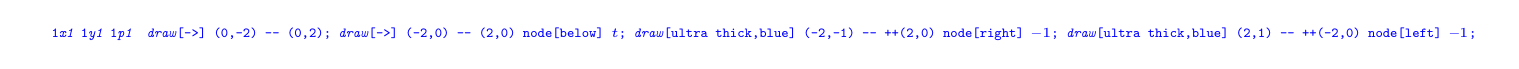
\begin{tikzpicture}
     \draw[->] (0,-2) -- (0,2);
     \draw[->] (-2,0) -- (2,0) node[below] {$t$};
     
     \draw[ultra thick,blue] (-2,-1) -- ++(2,0) node[right] {$-1$};
     \draw[ultra thick,blue] (2,1) -- ++(-2,0) node[left] {$-1$};
     \end{tikzpicture}
     
     \begin{align*}
     \mathrm{sgn}(t)&=\lim_{u\to0}\left[
     e^{-a|t|}\mathrm{sgn}(t)
     \right] \\
     \mathrm{ FT }\ \mathrm{sgn}(t) &=
     \int_{-\infty}^{\infty} e^{-a|t|}\mathrm{sgn}te^{-j\omega t}\dif t
     \\ &= \lim_{a\to0}\int_{-\infty}^{0} e^{at-j\omega t}\dif t
     + \lim_{a\to 0} \int_0^\infty e^{-at-j\omega t}\dif t
     \\ &=
     \lim_{a\to0}\left[ \left.-\frac{e^{(at-j\omega t)}}{a-j\omega }
     \right|_{-\infty}^0 + \left. \frac{e^{-at-j\omega t}}{-(a+j\omega )}
     \right|_0^\infty
      \right]
     \\ &= \lim_{a\to 0} \left[ \frac{-1}{a-j\omega }+\frac{1}{a+j\omega} \right]
     \\ &= \frac{2}{j\omega }\in\mathbb I
     \end{align*}
     
     \paragraph{}
     \begin{align*}
     u(t) &\xrightarrow{\text{F.T.}} \\
     u(t) &= \frac{1}{2}+\frac{1}{2}\mathrm{sgn}(t)
     \xrightarrow{\text{F.T.}} \pi\delta(\omega ) +\frac{1}{j\omega }
     \end{align*}
     
     
\begin{tikzpicture}
     \draw[->] (0,-1.5) -- (0,2) node[right] {$F(\omega)$};
     \draw[->] (-2,0) -- (2,0) node[below] {$\omega$};
     
     \draw[very thick,blue] plot [smooth,tension=1] coordinates {(-1.5,0) (0,1.2) (1.5,0)};
     
     \draw (1,-1) node[right] {$X(0) \to$ εκφράζει το D.C};
     \end{tikzpicture}
     
     \subsubsection{}     
     \begin{align*}
     \mathrm u(t) &\xrightarrow{\text{F.T.}} \pi\delta(\omega )+\frac{1}{j\omega }\\
     f(t) &\xrightarrow{\text{F.T.}} F(\omega ) \\
     g(t) &= \int_{-\infty}^{t}f(t)\dif t = \int_{-\infty}^{\infty} f(\tau)
     \mathrm u(t-\tau)\dif\tau = f(t)*\mathrm u(t) \\
     G(\omega ) &= F(\omega )\cdot\left[ \pi\delta(\omega )+\frac{1}{j\omega } \right]
     \end{align*}
     
     \subsubsection{}
     \begin{align*}
     \delta(t) &\to 1 \quad \text{άρτια} \\
     \delta^{(1)}(t)=\od{}{t}\delta(t) &\to j\omega \\
     \delta^{(n)}(t)=\od[n]{}{t}\delta(t) &\to (j\omega )^n
     \end{align*}
     \paragraph{}
     \begin{align*}
     t^n \to 2\pi j^n\delta^{(n)}(\omega )
     \end{align*}
     
     \subsubsection{}
     \paragraph{Παρ.}
     \begin{align*}
     f(t)&=|t| = t\mathrm u(t) - t\mathrm u(-t)\\
     F(\omega ) &= \frac{1}{2\pi}\left[
     2\pi j\delta(\omega )*\left[\pi\delta(\omega )+\frac{1}{j\omega }\right]
     -2\pi j \delta(\omega )*\left[ \pi\delta(\omega )-\frac{1}{j\omega } \right]
     \right]
     \end{align*}
     
     Calculate at home! The answer is \( -\frac{2}{\omega ^2} \)
     
     \begin{align*}
     t &\to 2\pi j^1\delta^{(1)}(\omega )\\
     \mathrm u(t) &\to \pi\delta(\omega )+\frac{1}{j\omega } \\
     \mathrm u(-t) &\to \pi\delta(\omega)-\frac{1}{j\omega }
     \end{align*}
     
     \subsubsection{Kramer's Kronig Relations}
     Από ηλεκτρομαγνητικό πεδίο: \[
       \underbrace{\vec D}_{\mathclap{\text{πυκνότητα ροής}}} = 
       \overbrace{\epsilon }^{\mathclap{\text{διηλεκτρική σταθερά}}}
       \underbrace{\vec E}_{\mathclap{\text{ένταση πεδίου}}}
     \]
     \begin{align*}
     \vec E =& \vec E(\vec r, t) \\
     &\vec E(\vec r,\omega ) \\
     \vec D(\omega ) =& \epsilon(\omega )\vec E(\omega )\\
     \vec D(t) =& \epsilon (t) +\vec E(t)
     \end{align*}
     
     \begin{tikzpicture}
     \draw[->] (0,-2) -- (0,0) node[left]
     {$\Im\left\lbrace \varepsilon(\omega)\right\rbrace$};
     \draw[->] (0,0) -- (0,2) node[left]
     {$\Re\left\lbrace \varepsilon(\omega)\right\rbrace$};
     
     \draw (0,0) -- (3,0);
     
     \draw[very thick,blue] (0,0.4) --
     plot [smooth, tension=1, domain=0.4:3, samples=9] (\x,{0.8+0.7*rand});
     
     \draw[very thick,blue!70!orange] (0,-0.2) --
     plot [smooth, tension=1, domain=0.4:3, samples=9] (\x,{-0.8+0.7*rand});
     \end{tikzpicture}
     
     \paragraph{}
     \begin{align*}
     h(t) &= 0 \quad \forall t < 0 \\
     h(t)&: \mathbb R \to \mathbb R
     \end{align*}
    
    Αν \( H(\omega ) = \mathscr F T\left\lbrace h(t) \right\rbrace = H_R(\omega )
    +jH_I(\omega )
     \)
     
     \begin{align*}
     \Aboxed{ H_I(\omega ) &= -\frac{1}{\pi} \int_{-\infty}^{\infty}
     \frac{H_R(\omega)}{\omega -\omega'}\dif \omega ' } \\
     \Aboxed{ H_R(\omega ) &= \frac{1}{\pi} \int_{-\infty}^{\infty}
     \frac{H_I(\omega )}{\omega -\omega'}\dif \omega' }
     \end{align*}
     
     Η απόδειξη των σχέσεων θα πέσει στις εξετάσεις.
     
     \paragraph{Άσκ.}
     \begin{align*}
     f(t) &= 2\cos\omega_1 t \cos\omega_2 t = \cos(\omega_1-\omega_2)t
     +\cos(\omega_1+\omega_2)t
     \\ F(\omega ) &= \mathscr F\left\lbrace 
     \cos(\omega_1-\omega_2)t
      \right\rbrace + \mathscr F \left\lbrace \cos(\omega_1+\omega_2)t \right\rbrace
      \\ &=
      \pi \left[
      \delta\left( \omega -(\omega_1-\omega_2) \right)
      +\delta\left( \omega +(\omega_1-\omega_2) \right)
      \right] + \pi \left[
      \delta\left( \omega -(\omega_1+\omega_2) \right)
      +\delta\left( \omega +(\omega_1+\omega_2) \right)
      \right] 
     \end{align*}
     
     \( \left( \cos\omega_0t \xrightarrow{\text{FT}}
     \pi\left[ \delta(\omega -\omega_0)+\delta(\omega+\omega_0) \right]
      \right) \)
     
     Εναλλακτικά:
     \begin{align*}
     F(\omega ) &= 2\frac{1}{2\pi}\mathscr F \left\lbrace \cos\omega_1 t \right\rbrace
     * \mathscr F\left\lbrace \cos\omega_2 t \right\rbrace \\
     &= \pi \left[ \delta(\omega -\omega_1)+\delta(\omega+\omega_1) \right]
     * \left[ \delta(\omega -\omega_2)+\delta(\omega+\omega_2) \right]
     \\ &= \pi \left[
     \delta(\omega-\omega_2-\omega_1) +\delta(\omega-\omega_2+\omega_1)
     +\delta(\omega+\omega_2+\omega_1)+\delta(\omega+\omega_2-\omega_1)
     \right]
     \end{align*}
     
     \paragraph{Άσκηση}
     \begin{align*}
     f(t) &= g(t) \cos^2 \omega_0 t \qquad g(t) \xrightarrow{\text{FT}} G(\omega )
     \\ &= g(t)\frac{1+\cos2\omega_0 t}{2} = \frac{g(t)}{2} + 
     \frac{1}{2}g(t)\cos2\omega_0 t \\
     \implies F(\omega ) &= \frac{1}{2}G(\omega )+\frac{1}{2}G(\omega )
     *\mathscr F\left\lbrace \cos2\omega_0 t \right\rbrace
     \\ &= \frac{1}{2}G(\omega )+\frac{1}{2}G(\omega ) *
     \left[ \pi\left(\delta(\omega-2\omega_0)+\delta(\omega+2\omega_0)\right) \right]
     \frac{1}{2\pi} \\ &= \frac{1}{2}G(\omega ) + \frac{1}{4} \left[
     G(\omega -2\omega_0)+G(\omega +2\omega_0)
     \right]
     \end{align*}
     
     Αν δεν θυμάμαι τον τύπο:
     \begin{align*}
     f(t) &= g(t)\cos^2\omega_0 t = g(t)\cos\omega_0 t\cos\omega_0 t \\
     F(\omega ) &= \frac{1}{2\pi}G(\omega)*\left[
     \frac{1}{2\pi}\mathscr F\left\lbrace \cos\omega_0t \right\rbrace
     *\mathscr F \left\lbrace \cos\omega_0 t \right\rbrace
     \right] \\ &= \frac{1}{4\pi^2} G(\omega ) * \left[
     \pi\left[ \delta(\omega -\omega_1)+\delta(\omega+\omega_2) \right]
     \right] * \pi\left[
     \delta(\omega-\omega_1)+\delta(\omega+\omega_2)
     \right] \\ &=
     \frac{1}{4}G(\omega ) * \left[
     \delta(\omega -2\omega_0)+\delta(\omega)+\delta(\omega)+\delta(\omega+2\omega_0)
     \right]
     \\ &= \frac{1}{4}\left[
     G(\omega -2\omega_1)+2G(\omega )+G(\omega +2\omega_0)
     \right]
     \end{align*}
     
     \paragraph{Άσκηση}
     \begin{align*}
     f(t) &= g(at+b) \qquad g(t)\xrightarrow{\text{FT}}G(\omega ) \\
     h(t)=g(at) \qquad
     F(\omega ) &= \mathscr F\left\lbrace g(at)+b \right\rbrace
     = \mathscr F \left\lbrace h\left(t+\frac{b}{a}\right) \right\rbrace
     = H(\omega )e^{j\omega \frac{b}{a}} \\[5pt]
     H(\omega ) &= \frac{1}{|a|}G\left(\frac{\omega}{a}\right) \\
     \Aboxed{F(\omega ) &=
     \frac{1}{|a|}e^{j\omega\frac{b}{a}}G\left(\frac{\omega}{a}\right)}
     \end{align*}
     
     \paragraph{}
     \begin{align*}
     \cos t &\xrightarrow{\text{FT}} \pi\left[
     \delta(\omega -1)+\delta(\omega +1)
     \right] \\
     \sin \omega_0 t &= \cos\left(\omega_0t-\frac{\pi}{2}\right)
     \\
     \sin t &\xrightarrow{\text{FT}}
     \frac{1}{|\omega_0|}e^{-j\omega\frac{\pi}{2\omega_0}}\pi
     \left[ \delta\left(\frac{\omega}{\omega_0}-1\right)
     +\delta\left(\frac{\omega}{\omega_0} + 1\right)
      \right]
      \\ &\overset{\mathllap{\delta\left(\frac{\omega}{\omega_0}-1\right)
        = \delta\left(\frac{1}{\omega_0}(\omega-\omega_0)\right)}
        }{=}
        e^{-j\frac{\omega}{\omega_0}}\pi\left[
        \delta(\omega-\omega_0)+\delta(\omega +\omega_0)
        \right] \\ &= -j\pi\left[
        \delta(\omega -\omega_0)-\delta(\omega+\omega_0)
        \right]
     \end{align*}
     
     \paragraph{}
     \hspace{0pt}
     
     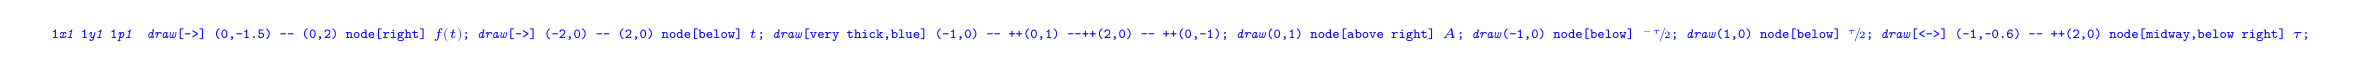
\begin{tikzpicture}
     \draw[->] (0,-1.5) -- (0,2) node[right] {$f(t)$};
     \draw[->] (-2,0) -- (2,0) node[below] {$t$};
     
     \draw[very thick,blue] (-1,0) -- ++(0,1) --++(2,0) -- ++(0,-1);
     \draw (0,1) node[above right] {$A$};
     
     \draw (-1,0) node[below] {$\sfrac{-\tau}{2}$};
     \draw (1,0) node[below] {$\sfrac{\tau}{2}$};
     
     \draw[<->] (-1,-0.6) -- ++(2,0) node[midway,below right] {$\tau$};

     \end{tikzpicture}
     
     \begin{align*}
     F(\omega ) &= \int_{-\infty}^{\infty} f(t)e^{-j\omega t}\dif t
     = A \int_{-\sfrac{\tau}{2} }^{\sfrac{\tau}{den} }e^{-j\omega t}\dif t
     \\ &= A\frac{1}{-j\omega }
     \left. e^{-j\omega t}\right|_{\sfrac{\tau}{2}}^{\sfrac{\tau}{2}}
     =\frac{A}{-j\omega }\left[ e^{-j\omega \sfrac{\tau}{2} } 
     -e^{j\omega \sfrac{\tau}{2}}
     \right] \\ &= A\tau\frac{\sin\left(\omega\frac{t}{2}\right)}{\frac{\omega t}{2}}
     \\ &= A\tau\frac{\sin\left(\frac{\omega t}{2}\right)}{\frac{\omega t}{2}}
     =A\tau \mathrm{sinc}\left(\frac{\omega t}{2\pi}\right)
     \end{align*}
     \begin{infobox}{sinc}
        \vspace{-5pt}
        \begin{align*}
        \text{Μαθηματικοί:}\quad \mathrm{sinc}(x)&=\frac{\sin x}{x}\\
        \text{Μηχανικοί:}\quad \mathrm{sinc}(x)&=\frac{\sin(\pi x)}{\pi x}
        \end{align*}
     \end{infobox}
     
     \subsection{Χρονοπερατό vs Ζωνοπερατό Σήμα}
     \begin{center}
     \begin{tikzpicture}
     \draw[->] (0,0) -- (0,2) node[right] {$f(t)$};
     \draw[->] (-3,0) -- (3,0) node[below] {$t$};
     
     \draw[very thick,blue] 
     plot[smooth] coordinates {(-2,0) (-1.9,0.5) (-1.7,0.7) (-1.5,0.4) (-1.2, 0.7)  
     	(-1, 0.9) (-0.8,0.1) (-0.5,0.5) (-0.3,0.5) (-0.1,0.7) (0,0.6) (0.1,0.8) (0.3,1.1)
     	(0.5,0.8) (0.6,0.9) (0.8,0.7) (1,0.5) (1.2,0.6) (1.5,0)
     } ;
     
     \draw (-2,0) node[below] {$A$};
     \draw (1.5,0) node[below] {$B$};
     
     \draw[<->] (-2,-0.5) -- ++(3.5,0) node[midway,below] {$T$};
     
     \draw (0,-1.2) node {$T$-timelimited};
     
     \begin{scope}[xshift=10cm]
     \draw[->] (0,-0.5) -- (0,2) node[right] {$G(\omega)$};
     \draw[->] (-2,0) -- (2,0) node[below] {$\omega$};
     
     \draw[very thick,blue] plot[smooth,tension=1.2] coordinates {(-1,0) (0,1) (1,0)};
     
     \draw (-1,0) node[below] {$\sfrac{-\sigma}{2}$};
     \draw (1,0) node[below] {$\sfrac{\sigma}{2}$};
     
     \draw (0,-1.2) node {$\sigma$-bandlimited};
     \end{scope}
     \end{tikzpicture}
     \end{center}
     
     \begin{itemize}
        \item Ένα ζωνοπερατό σήμα \textbf{δεν} μπορεί να είναι χρονοπερατό
        \item Ένα χρονοπερατό σήμα \textbf{δεν} μπορεί να είναι ζωνοπερατό
        \item Ένα σήμα μπορεί να μην είναι ούτε χρονοπερατό, ούτε ζωνοπερατό.
     \end{itemize}
     
     \begin{tikzpicture}
     \draw[gray,dashed] (-1,0) -- ++(0,-4);
     \draw[gray,dashed] (1,0) -- ++(0,-4);
     
     \draw[->] (0,-0.5) -- (0,2) node[right] {$f(t)$};
     \draw[->] (-2,0) -- (2,0) node[below] {$t$};
     
     \draw[very thick,blue] plot[smooth,tension=1.2] coordinates {(-1,0) (0,1) (1,0)};
     
     \draw (3,1) node {χρονοπερατό};
     
     \begin{scope}[yshift=-4cm]
     \draw[->] (0,-0.5) -- (0,2) node[right] {$f(t)$};
     \draw[->] (-2,0) -- (2,0) node[below] {$t$};
     
     \draw[very thick,blue] plot[smooth] 
     coordinates { (-2,-0.5) (-1,0) (0,1) (1,0) (2,-0.7)};
     
     \draw (3,1) node {ζωνοπερατό};
     
     \begin{scope}[xshift=6cm]
     \draw[->] (0,-0.5) -- (0,2) node[right] {$\hat f(\omega)$};
     \draw[->] (-2,0) -- (2,0) node[below] {$\omega$};
     
     \draw[very thick,blue] plot[smooth,tension=2] coordinates {(-1,0) (0,1.2) (1,0)};
     \end{scope}
     \end{scope}
     \end{tikzpicture}
     
     \paragraph{Απόδ.}
     \hspace{0pt}
     
   	\begin{tikzpicture}
   	\draw[->] (0,-0.5) -- (0,2) node[right,style={align=left}]
   	{Ζωνοπερατό\\$F(\omega)$};
   	\draw[->] (-2,0) -- (2,0) node[below] {$\omega$};
   	
   	\draw[very thick,blue] plot[smooth,tension=2] coordinates {(-1,0) (0,1.2) (1,0)};
   	
   	\draw (-1,0) node[below] {$\sfrac{-\sigma}{2}$};
   	\draw (1,0) node[below] {$\sfrac{\sigma}{2}$};
   	
   	\draw[->,thick] (2,1) -- ++(2,0) node[midway,above] {ΕΣΤΩ};
   	
   	\begin{scope}[xshift=6cm]
   	\draw[->] (0,-0.5) -- (0,2) node[right,style={align=left}]
   	{Χρονοπερατό\\$f(t)$};
   	\draw[->] (-2,0) -- (2,0) node[below] {$t$};
   	
   	\begin{scope}[xscale=1.3]
   	\draw[very thick,blue] plot[smooth,tension=1] coordinates {(-1,0) (0,1) (1,0)};
   	
   	\draw (-1,0) node[below] {$\sfrac{-T}{2}$};
   	\draw (1,0) node[below] {$\sfrac{T}{2}$};
   	\end{scope}
   	\end{scope}
   	
   	\end{tikzpicture}
     \begin{align*}
     f(t) &= \int_{-\sfrac{\sigma}{2} }^{\sfrac{\sigma}{2} } F(\omega )
     e^{j\omega t}\dif\omega \\
     \od[n]{f(t)}{t} &= \int_{-\sfrac{\sigma}{2} }^{\sfrac{\sigma}{2} }
     (j\omega )^n F(\omega )e^{j\omega t}\dif\omega
     \end{align*}
     Ορίζεται η σειρά Taylor επομένως σε οποιοδήποτε σημείο, όμως τότε, επειδή
     σε κάποια σημεία οι παράγωγοι είναι 0, θα έπρεπε η \( F \) να είναι
     μηδενική, άτοπο.
     
     \subsection{Γκαουσιανός παλμός}
     \[
     f(t) = \frac{1}{\sigma\sqrt{2\pi}}
     e^{\sfrac{t^2}{(2\sigma^2)} } \quad \xrightarrow{\quad\text{FT}\quad}
     F(\omega ) = e^{\frac{1}{2}\omega^2\sigma^2}
     = e^{-\frac{1}{2\frac{1}{\sigma^2}}\omega^2}
     \]
     
     \begin{center}
     \begin{tikzpicture}[scale=1.5]
     \draw[->] (0,-1) -- (0,2) node[right] {$f(t)$};
     \draw[->] (-2,0) -- (2,0) node[below] {$t$};
     
     \draw[thick,green!60!black,<->] (-0.9,0.5) -- (0.9,0.5) node[below right,midway]
     {$\sigma^2$};
     
     \draw[ultra thick,samples=50,domain=-2:2,yscale=1.2,smooth,variable=\x,blue] 
     plot ({\x},{  exp(-\x*\x)  });
     
     \begin{scope}[xshift=6cm]
     \draw[->] (0,-1) -- (0,2);
     \draw[->] (-2,0) -- (2,0) node[below] {$t$};
     
     \draw[ultra thick,samples=50,domain=-2:2,yscale=1,smooth,variable=\x,blue!50!black] 
     plot ({\x},{  exp(-\x*\x/3)  });
     \draw[ultra thick,samples=50,domain=-2:2,yscale=1.4,smooth,variable=\x,
     blue!50!green] 
     plot ({\x},{  exp(-\x*\x*4)  });
     
     \draw[green!60!black,->] (0.1,{exp(-0.1^2*4)*1.4}) to[bend left=20] (0.8,2) node[right]
     {$\sigma_1$};
     \draw[green!60!black,->] (0.7,{exp(-0.7^2/3)}) to[bend left] (1.2,1.5) node[right]
     {$\sigma_2>\sigma_1$};
     \end{scope}

     \end{tikzpicture}
     \end{center}
     
     \begin{gather*}
     {\textstyle \int_{-\infty}^{\infty} f(t)\dif t = 1} \\
     \sigma^2 \text{ διασπορά}
     \end{gather*}
     \begin{align*}
     F(\omega ) &= \int_{-\infty}^{\infty} f(t)e^{-j\omega t}\dif t
     =\frac{1}{\sigma\sqrt{2\pi}}\int_{-\infty}^{\infty}
     e^{-\frac{t^2}{2\sigma^2}-j\omega t}\dif t
     \\ &= \frac{1}{\sigma\sqrt{2\pi}}\int_{-\infty}^{\infty}
     e^{-\frac{1}{\sigma^2}\left[
        t^2+2\sigma^2j\omega t+(j\omega \sigma^2)^2
        \right]}\cdot e^{\frac{1}{2\sigma^2}\left(j\omega \sigma^2\right)^2}\dif t
     \\ &=\frac{1}{\sigma\sqrt{2\pi}}e^{-\frac{1}{2\sigma^2}\omega^2\sigma^4}
     \int_{-\infty}^{\infty} e^{-\frac{1}{2\sigma^2} 
        \overbrace{\textstyle\left(t+j\omega\sigma^2\right)}^{t+j\omega\sigma^2-\tau}
        }\dif t
        \\ &= e^{-\frac{1}{2}\omega^2\sigma^2}\boxed{
            \frac{1}{\sigma\sqrt{2\pi}}\int_{-\infty}^{\infty}
            e^{-\frac{2}{\sigma^2}\tau^2}\dif\tau
            } = \displaystyle e^{\displaystyle -\frac{1}{2}\omega^2\sigma^2}
     \end{align*}
     
     Ηθικά διδάγματα:
     \begin{itemize}
        \item Ο μετασχηματισμός της Gaussian είναι Gaussian
        \item Ό,τι στενεύει στον χρόνο απλώνει στο φάσμα, και αντίθετα
     \end{itemize}
     \begin{center}
     		\begin{tikzpicture}
     		\draw[thick,green!60!black,<->] (-0.9,0.5) -- (0.9,0.5);
     		
     		\draw[very thick,samples=50,domain=-2:2,yscale=1.2,smooth,variable=\x,blue] 
     		plot ({\x},{  exp(-\x*\x)  });
     		
     		\draw[->] (0,-1) -- (0,2) node[right] {$f(t)$};
     		\draw[->] (-2,0) -- (2,0) node[below] {$t$};
     		
     		\draw (-0.9,0.5) node[above left,black] {$\sigma_1^2$};
     		
     		\draw[->,thick] (2,1) -- ++(2,0) node[midway,above] {FT};
     		
     		\begin{scope}[xshift=6cm]
     		
     		\draw[very thick,samples=50,domain=-2:2,yscale=1.2,smooth,variable=\x,blue] 
     		plot ({\x},{  exp(-\x*\x/1.2)  });
     		
     		\draw[->] (0,-1) -- (0,2) node[right] {$F(\omega)$};
     		\draw[->] (-2,0) -- (2,0) node[below] {$\omega$};
     		
     		\draw (0.9,0.5) node[above right,black] {$\frac{1}{\sigma_1^2}$};
     		\end{scope}
     		
     		\begin{scope}[yshift=-4cm]    
     		\draw[very thick,samples=50,domain=-2:2,yscale=1.2,smooth,variable=\x,blue] 
     		plot ({\x},{  exp(-\x*\x/3)  });
     		
     		\draw[->] (0,-1) -- (0,2) node[right] {$f(t)$};
     		\draw[->] (-2,0) -- (2,0) node[below] {$t$};
     		
     		\draw (1.2,0.5) node[above right,black] {$\sigma_2^2>\sigma_1^2$};
     		
     		\draw[->,thick] (2,1.2) -- ++(2,0) node[midway,above] {FT};
     		
     		\begin{scope}[xshift=6cm]
     		
     		\draw[very thick,samples=50,domain=-2:2,yscale=1.2,smooth,variable=\x,blue] 
     		plot ({\x},{  exp(-\x*\x/1.2*3)  });
     		
     		\draw[->] (0,-1) -- (0,2) node[right] {$F(\omega)$};
     		\draw[->] (-2,0) -- (2,0) node[below] {$\omega$};
     		
     		\draw (0.9,0.5) node[above right,black]
     		{$\frac{1}{\sigma_2^2} > \frac{1}{\sigma_1^2}$};
     		\end{scope}
     		\end{scope}
     		
     		\end{tikzpicture}
     \end{center}
     
     \paragraph{}
     \begin{gather*}
     \int_{-\infty}^{\infty} td^2(t)\dif t \\
     \text{διασπορά στον χρόνο} \quad d^2 = \int_{-\infty}^{\infty} t^2f^2(t)\dif t\\
     \text{διασπορά στο φάσμα}\quad D^2=\frac{1}{2\pi}
     \int\omega^2\left|\right|\dif\omega \\
     \left|\int_{-\infty}^{\infty} tx(t)\od{x(t)}{t}\dif t\right|
     \leq \int_{-\infty}^{\infty} t^2x^2(t)\dif t \cdot
     \int_{-\infty}^{\infty}\left|\od{x(t)}{t}\right|\dif t 
     \overset{\text{Parseval theorem}}{=} d^2D^2
     \implies \boxed{dD \geq \sfrac{1}{2} }
     \end{gather*}
     
     Γιατί \( \sfrac{1}{2}  \); (Υπόδειξη: \( 
     \int_{-\infty}^{\infty} tx\od{x}{t}\dif t =
     \int_{-\infty}^{\infty} t \frac{1}{2}\od{x^2}{t}\dif t
     = \left[ \quad \right] - \cancelto{1}{\frac{1}{2}\int x^2\dif t}
      \))
      
    Θα τα ξαναπούμε Τρίτη 22 Νοεμβρίου (χάνουμε 3 μαθήματα).

	    \section{Μετασχηματισμός Laplace}
    \begin{align*}
        \nexists\, X(\omega ) &= \int_{-\infty}^{\infty} x(t)e^{-j\omega t}\dif t\\
        y(t) &= x(t)e^{-\sigma t}\\
        \exists\, Y(\omega ) &= \int_{-\infty}^{\infty} y(t)e^{-j\omega t}\dif t
        \quad (s=\sigma+j\omega ) \\ &= \int_{-\infty}^{\infty} x(t)
        e^{-\sigma t}e^{-j\omega t}\dif t \\
        \Aboxed{ X(s) &= \int_{-\infty}^{\infty} x(t)e^{-st}\dif t }
        \quad \text{Μ. Laplace}
    \end{align*}
    
    \paragraph{Αντίστροφος μετασχηματισμός Laplace}
    \( \displaystyle
    x(t) = \frac{1}{2\pi j}
    \int_{\sigma-j\underset{\mathclap{(-\infty)}}{\omega} }^{
        \sigma+j\overset{\mathclap{(\infty)}}{\omega}} X(s)e^{st}\dif s
     \)
     
     \paragraph{}
     
    \begin{itemize}
        \item Έστω ότι \( x(t) \) είναι αιτιατή (\( x(t)=0 \quad t< 0 \)).
        
        Ας φανταστούμε ότι η \( x(t) \) δεν έχει μετασχηματισμό Fourier.
        
        \begin{tikzpicture}[scale=1,xscale=1]
        \fill[samples=30,domain=0:4,smooth,variable=\x,blue!10] 
        plot ({\x},{exp(\x/2-1)}) -- (4,0) -- (0,0) -- cycle;
        \fill[samples=30,domain=0:4,smooth,variable=\x,blue!10] 
        plot ({\x},{-exp(\x/2-1)}) -- (4,0) -- (0,0) -- cycle;
        
        \draw[->] (0,-2) -- (0,2); %node[right] {$f(t)$};
        \draw[->] (-2,0) -- (4,0) node[below,right] {$t$};
        
        \draw[samples=100,domain=4:0,smooth,variable=\x,blue,very thick] 
        plot ({\x},{-exp(\x/2-1)* sin(-5*\x r)});
        \draw[samples=50,domain=4:0,smooth,variable=\x,blue] 
        plot ({\x},{exp(\x/2-1)}) plot ({\x},{-exp(\x/2-1)});
        
        \draw (0,-2) node[below] {$x(t) = \sin( \omega t)\, e^t \mathrm u(t)$};
        
        \begin{scope}[xshift=7cm]
        \fill[green!70] (1,-2) rectangle (0.7,2);
        \fill[green!70,path fading=east] (2,-2) rectangle (1,2);
        
        \draw[->] (-2,0) -- (2,0) node[below] {$\sigma$};
        \draw[->] (0,-2) -- (0,2) node[right] {$j\omega$};
        
        \draw[dashed] (0.7,-2) -- ++(0,4);
        \draw (0.7,0) node[above left] {$1$};
        
        \draw (-1,-1) node {$s$-plane};
        \draw (2,-1) node {$\Re\lbrace s\rbrace = \sigma>1$};
        \end{scope}
        \end{tikzpicture}
        
        \vspace{5pt}
        
        \begin{tikzpicture}[scale=1,xscale=1]
        \fill[samples=30,domain=0:4,smooth,variable=\x,blue!10] 
        plot ({\x},{exp(-\x/1.5+0.5)}) -- (4,0) -- (0,0) -- cycle;
        \fill[samples=30,domain=0:4,smooth,variable=\x,blue!10] 
        plot ({\x},{-exp(-\x/1.5+0.5)}) -- (4,0) -- (0,0) -- cycle;
        
        \draw[->] (0,-2) -- (0,2); %node[right] {$f(t)$};
        \draw[->] (-2,0) -- (4,0) node[below,right] {$t$};
        
        \draw[samples=100,domain=4:0,smooth,variable=\x,blue,very thick] 
        plot ({\x},{-exp(-\x/1.5+0.5)* sin(-5*\x r)});
        \draw[samples=50,domain=4:0,smooth,variable=\x,blue] 
        plot ({\x},{exp(-\x/1.5+0.5)}) plot ({\x},{-exp(-\x/1.5+0.5)});
        
        \draw (0,-2) node[below] {$x(t) = \sin( \omega t)\, e^{-t} \mathrm u(t)$};
        
        \begin{scope}[xshift=7cm]
        \fill[green!70] (-0.3,-2) rectangle (-0.7,2);
        \fill[green!70,path fading=east] (-0.3,-2) rectangle (2,2);
        
        \draw[->] (-2,0) -- (2,0) node[below] {$\sigma$};
        \draw (0,-2) -- (0,2);
        
        \draw[dashed] (-0.7,-2) -- ++(0,4);
        \draw (-0.7,0) node[above left] {$-1$};
        
        \draw (2,-1) node {$\Re\lbrace s\rbrace = \sigma>-1$};
        \end{scope}
        \end{tikzpicture}
        
        \item Έστω ότι \( x(t) \) αντιαιτιατή (\( x(t)=0 \quad t>0 \))
        
        \begin{tikzpicture}[scale=1,xscale=1]
        
        \fill[samples=30,domain=-4:0,smooth,variable=\x,blue!10] 
        plot ({\x},{exp(-\x/2-1)}) -- (0,0) -- (-4,0) -- cycle;
        \fill[samples=30,domain=-4:0,smooth,variable=\x,blue!10] 
        plot ({\x},{-exp(-\x/2-1)}) -- (0,0) -- (-4,0) -- cycle;
        
        \draw[->] (0,-2) -- (0,2); %node[right] {$f(t)$};
        \draw[->] (-4,0) -- (3,0) node[below,right] {$t$};
        
        \draw[samples=100,domain=-4:0,smooth,variable=\x,blue,very thick] 
        plot ({\x},{-exp(-\x/2-1)* sin(5*\x r)});
        \draw[samples=50,domain=-4:0,smooth,variable=\x,blue] 
        plot ({\x},{exp(-\x/2-1)}) plot ({\x},{-exp(-\x/2-1)});
        
        \draw (0,-2) node[below] {$x(t) = \sin \omega t\, e^{-t} \mathrm u(-t)$};
        
        \begin{scope}[xshift=6cm]
        \fill[green!70] (-1,-2) rectangle (-0.7,2);
        \fill[green!70,path fading=west] (-2,-2) rectangle (-1,2);
        
        \draw[->] (-2,0) -- (2,0);
        \draw (0,-2) -- (0,2);
        
        \draw[dashed] (-0.7,-2) -- ++(0,4);
        \draw (-0.7,0) node[above right] {$-1$};
        
        \draw (1,1) node {$s$-plane};
        \end{scope}
        \end{tikzpicture}

        
        \item \mbox{}
        \\
        \begin{tikzpicture}[scale=1,xscale=0.5]
        
        \fill[green!70,path fading=east] (0,-2) rectangle (5,2) ;
        
        \draw (-2,0) -- (4,0);
        \draw (0,-2) -- (0,2);
        
        \draw (0,0) node[below left] {$\mathsmaller{0}$};
        
        \draw (0,-2) node[below right] {$\Re \lbrace s \rbrace \geq 0 $};
        
        \begin{scope}[xshift=9cm]
        \fill[green!50!blue!70!white,path fading=west] (1,-2) rectangle (-3,2) ;
        
        \draw (-2,0) -- (4,0);
        \draw (0,-2) -- (0,2);
        
        \draw (1,0) node[below right] {$1$};
        
        \draw (0,-2) node[below right] {$\Re \lbrace s \rbrace < 1$};
        \draw[dashed] (1,-2) -- ++(0,4);
        \end{scope}
        
        \begin{scope}[xshift=16cm]
        \fill[green!70!blue!50!white] (1,-2) rectangle (0,2) ;
        
        \draw (-2,0) -- (4,0);
        \draw (0,-2) -- (0,2);
        
        \draw (1,0) node[below right] {$1$};
        \draw[dashed] (1,-2) -- ++(0,4);
        \end{scope}
        
        \draw (current bounding box.north west) node[above right]
        {$\sin \omega t\, \mathrm u(t) + \sin \omega t\, e^t \mathrm u(-t)$};
        \end{tikzpicture}
        
        \item Η \( \sin \omega \mathrm u(t)+\sin\omega t e^{-t}\mathrm u(-t) \)
        δεν έχει περιοχή σύγκλισης.
    \end{itemize}
    
    \[
    X(s) = \frac{35}{(x-8)(x+2)}
    \]
    
    \begin{tikzpicture}[scale=1,xscale=0.5]
    
    \fill[green!30] (-4,-2) rectangle (-2.5,2) node[black,pos=.5,above] {$x_2(t)$};
    \fill[blue!30] (-2.5,-2) rectangle (1.5,2) node[black,pos=.5,below] {$x_3(t)$};
    \fill[orange!30] (1.5,-2) rectangle (4,2) node[black,pos=.5,above] {$x_1(t)$};
    
    \draw (-4,0) -- (4,0);
    \draw [dashed](-2.5,-2) -- ++(0,4);
    \draw[dashed] (1.5,-2) -- ++(0,4);
    \end{tikzpicture}
    
    Οι πόλοι (ρίζες του παρονομαστή) καθορίζουν τις περιοχές σύγκλισης.
    
    \paragraph{}
    Οι συναρτήσεις που χρησιμοποιούμε είναι αιτιατές, άρα γενικά ο μετασχηματισμός
    Laplace καταρρέει στην:
    \[
    X(s) = \int_{0^-}^{\infty} x(t)e^{-st}\dif t
    \]
    
    Το \( 0^- \) μάς επιτρέπει να ασχοληθούμε με συναρτήσεις που απειρίζονται
    στο 0, π.χ. \( \frac{1}{x} \) or \( \delta(t) \).
    
    \subsection{Ιδιότητες}
    \( x(t)\to X(s) \quad \Re\left\lbrace s \right\rbrace > \sigma_1 \)
    
    \( y(t)\to\, Y(s) \quad \Re\left\lbrace s \right\rbrace > \sigma_2 \)
    
    \begin{enumpar}
    \item \(\displaystyle ax(t)+by(t) \to aX(s)+bY(s) \qquad \text{τουλάχιστον }
    \Re\left\lbrace s \right\rbrace >
     \max\left\lbrace \sigma_1,\sigma_2 \right\rbrace\)
     \item Μετατόπιση σε χρόνο
    \begin{align*}
    x(t)\mathrm u(t)\to X(s)\quad & \sigma>\sigma_1 \\
    y(t) = x(t-t_0)\mathrm u(t-t_0)\to X(s)e^{-t_0s} 
    \quad & t_0>0 \quad \sigma>\sigma_2
    \end{align*}
    \subparagraph{Απόδ.}
    \begin{align*}
    Y(s) = \int_{0^-}^\infty y(t)e^{-st}\dif t
    = \int_{0^-}^{\infty} x(\underbrace{t-t_0}_{\tau})\mathrm u(t-t_0)e^{-st}\dif t
    = x(\tau)\mathrm u(\tau)e^{-s(t+t_0)}\dif\tau = X(s)e^{-st_0}
    \end{align*}
    \item Κλιμάκωση
    \begin{gather*}
    x(t)\to X(s) \\
    x(at)\to\frac{1}{a}X\left(\frac{s}{a}\right)\quad a>0
    \end{gather*}
    \item Παραγώγιση
    \begin{gather*}
    x(t)\to X(s) \\
    \od{x(t)}{t}\to sX(s)-x\left(0^- \right)
    \end{gather*}
    \item Ολοκλήρωση
    \begin{gather*}
    x(t)\to X(s) \\
    \int_0^t x(t)\dif t \to \frac{1}{s}X(s)
    \end{gather*}
    \item Διαμόρφωση
    \begin{align*}
    x(t)\to X(s) &\qquad \sigma>\sigma_1 \\
    e^{-at}x(t)\to X(s+a) &\qquad 
    a\in\mathbb C \qquad \sigma>\sigma_1 - \Re\left\lbrace a \right\rbrace
    \end{align*}
    \item Συνέλιξη
    \begin{gather*}
    x(t)\to X(s)\\
    y(t) \to Y(s)
    \end{gather*}
    \[
    x(t)*y(t)=X(s)Y(s)
    \]
    \end{enumpar}
    
    \subsection{Laplace "περιοδικών συναρτήσεων"}
    \[
    x_T(t)=\begin{cases}
    x(t) &\quad 0\leq x \leq T \\
    0 &\quad \text{αλλού}
    \end{cases}
    \]
    
    \begin{tikzpicture}[scale=0.8,xscale=0.5]
    
    \begin{scope}
    \draw[->] (0,-0.5) -- (0,2) node[right] {$x(t)$};
    
    \draw[samples=50,domain=0:pi,smooth,variable=\x,blue,very thick] 
    plot ({\x},{sin(\x r)}) -- (2*pi,0);
    \draw[samples=50,domain=2*pi:3*pi,smooth,variable=\x,blue,very thick] 
    plot ({\x},{sin(\x r)}) -- (4*pi,0);
    \draw[samples=50,domain=4*pi:5*pi,smooth,variable=\x,blue,very thick] 
    plot ({\x},{sin(\x r)}) -- (6*pi,0);
    
    \draw[->] (-0.5,0) -- (6*pi+0.4,0) node[below,right] {$t$};
    \end{scope}
    
    \begin{scope}[yshift=-3cm]
    \draw[->] (0,-0.5) -- (0,2); %node[right] {$f(t)$};
    \draw[->] (-0.5,0) -- (6*pi,0) node[below,right] {$t$};
    
    \draw (6,0) node[below] {$T$};
    \draw(pi/2,1) node[above right] {$x_p(T)$};
    
    \draw[very thick, blue] (pi-0.01,0) -- (6,0);
    
    \draw[samples=200,domain=0:pi,smooth,variable=\x,blue,very thick] 
    plot ({\x},{sin(\x r)});
    
    \end{scope}
    
    \end{tikzpicture}
    
    \begin{align*}
    x(t)&=x_T(t)+x_T(t-T)+x_T(t-2T)+\dots\\
    x(t)&= \sum_{n=0}^\infty x_T (t-nT) \\
    \mathscr L\left\lbrace x(t) \right\rbrace &= \sum_{n=0}^\infty
    \mathscr L \left\lbrace x_T(t-uT) \right\rbrace \\[3pt]
    x_T(t) &\xrightarrow{\mathscr L} X^T(s)\\
    x_T(t-nT) &\xrightarrow{\mathscr L} X^T(s)e^{-nTs} \\
    \mathscr L\left\lbrace x(t) \right\rbrace
    &= \sum_{n=0}^\infty X^T(s)e^{-nTs}
    = X^T(s)\sum_{n=0}^\infty e^{-nTs} = \frac{1}{1-e^{-Ts}}X^T(s)
    \quad \sigma>\max(0,\sigma_1)
    \end{align*}
    
    \paragraph{}
    \( \displaystyle X(s) \xrightarrow{?} X(\omega ) \)
    
    \[
    X(\omega ) = \left. X(s)\right|_{s=j\omega }
    \]
    
    \paragraph{Ex. 1}
    \( x(t)= e^{-at}\mathrm ut() \)
    
    \( \displaystyle
    X(s) = \int_{0^-}^\infty x(t)e^{-st}\dif t
    =\int_{0^-}^\infty e^{-at}e^{-st}\dif t
    = \int_{0^-}^\infty e^{-(a+s)t}\dif t
    =\left. \frac{e^{-(a+s)t}}{-(a+s)}\right|_0^\infty
    = \frac{\cancelto{0}{e^{-(a+s)\infty}} -\cancelto{1}{e^{-(a+s)0}} }{-(a+s)}
    = \boxed{\frac{1}{s+a} \quad 
        \Re\left\lbrace s \right\rbrace > \Re\left\lbrace a \right\rbrace}
     \)
     
     
   \paragraph{Ex. 2}
   \( x(t)=\delta(t) \)
   
   \( \displaystyle
   X(t) = \int_{0^-}^\infty \delta(t)e^{-st}\dif t = e^{-s0} = 1 \quad s\in\mathbb C 
    \)
    
   \paragraph{Ex. 3}
   \( x(t)=\mathrm u(t) \qquad X(s)=\frac{1}{s} 
   \quad \Re\left\lbrace s \right\rbrace > 0\)
   
   Για να βρω πεδίο σύγκλισης: \( \displaystyle
   X(s) =
   \int_{0^+}^\infty 1e^{-st}\dif t = \left.
   \frac{e^{-st}}{-s}\right|_{0^-}^\infty
   = \frac{e^{-s\infty}-\cancelto{1}{e^{-s0}}}{-s}=\frac{1}{s}
    \)
    
   \paragraph{Ex. 4}
   \( x(t)=\cos\omega_0 t\, \mathrm u(t) \)
   
   \( \displaystyle
   x(t) = \frac{e^{j\omega_0 t}+e^{-j\omega_0 t}}{2}\, \mathrm u(t)
   =\frac{1}{2}e^{j\omega_0 t}\mathrm u(t)
   +\frac{1}{2}e^{-j\omega_0 t}\mathrm u(t)
   \xrightarrow{\mathscr L \mathrm T}
    \frac{1}{2}
    \underset{\sigma >0}{\frac{1}{s-j\omega_0}}+
    \underset{\sigma >0}{\frac{1}{2}\frac{1}{s+j\omega_0}}
    = \frac{1}{2} \frac{2s}{s^2+\omega_0^2}
    =\frac{s}{s^2+\omega_0^2} \quad \Re\left\lbrace s \right\rbrace>0
    \)
    
    \paragraph{Ex. 5}
    \( x(t)=\sin\omega_0 t\, \mathrm u(t) \)
    
    \( \displaystyle
    \frac{1}{2j}\left[
    e^{j\omega_0 t}\mathrm u(t)-e^{-j\omega_0 t}\mathrm u(t)
    \right] \xrightarrow{\mathscr L \mathrm T}
    \frac{1}{2j}\underset{\Re\left\lbrace s \right\rbrace>0}{
        \left[ \frac{1}{s-j\omega_0} - \frac{1}{s+j\omega_0} \right]
    } = \frac{\omega_0}{s^2+\omega_0^2}
     \qquad \Re \left\lbrace s \right\rbrace > 0
     \)
     
    Ποιός είναι ο μετασχηματισμός Fourier της παραπάνω;
    
    Το πιθανό λάθος αποτέλεσμα είναι το \( 
    \displaystyle \left(
    \xrightarrow[s=j\omega ]{FT} \frac{\omega_0}{\omega_0^2-\omega^2}
    \right)
     \)
     
    \( x(t) = \sin\omega_0t\, \mathrm u(t) \)
    
    \begin{align*}
    \sin\omega_0 t &\xrightarrow{\mathrm{FT}} j\pi\left[
    -\delta(\omega-\omega_0)+\delta(\omega +\omega_0)
    \right] \\
    \mathrm u(t) &\xrightarrow{\mathrm{FT}} \pi\delta(\omega )+\frac{1}{j\omega }
    \end{align*}
    \begin{align*}
    x(t) &\to \left[
    j\pi\left(\delta(\omega +\omega_0)-\delta(\omega -\omega_0) \right)
    \right] * \left[
    \pi\delta(\omega )+\frac{1}{j\omega }
    \right] \\
    &= \frac{1}{2\pi}\left[
    j\pi^2\left(
    \delta(\omega+\omega_0)-\delta(\omega-\omega_0)
    \right) +j\pi\left(
    \frac{1}{j(\omega+\omega_0)}-\frac{1}{j(\omega+\omega_0)}
    \right)    \right]
    \\ &= \frac{j\pi}{2}\left[
    \delta(\omega +\omega_0)-\delta(\omega-\omega_0)\right]+\left[
    \frac{\omega_0}{\omega_0^2-\omega^2}
    \right] 
    \end{align*}
    
    \begin{theorem*}[title=Θεωρήματα Αρχικής \& Τελικής Τιμής,width=.5\textwidth]%
        {Αρχικής \& Τελικής Τιμής}
    \begin{align*}
    \lim_{t\to 0^+} x(t) &= \lim_{s\to \infty} \left( sX(s) \right) \\
    \lim_{t\to \infty} x(t) &= \lim_{s\to 0} \left( sX(s) \right)
    \end{align*}
    \end{theorem*}
    
    \begin{gather*}
    (-t)^n f(t) \xrightarrow{\mathscr L T} \od[n]{F(s)}{s} \\
    f(t) \xrightarrow{\mathscr L T} F(s)
    \end{gather*}
    
    Για να βρίσκουμε αντίστροφους μετασχηματισμούς Laplace χωρίς μιγαδική
    ολοκλήρωση χρειαζόμαστε ένα ισχυρό τυπολόγιο.
    
    \begin{infobox}{Τυπολόγιο}
    \[
    \begin{array}{cc}
        X(s) & x(t) \\ \hline
        \frac{1}{s} & \mathrm u(t) \\ \hline
        \frac{1}{s+a} & e^{-at}\mathrm u(t) \\ \hline
        \frac{1}{(s+a)^n} & \frac{t^{n-1}}{(n-1)!}e^{-at}\mathrm u(t) \\ \hline
        \frac{1}{s^n} & \frac{t^{n-1}}{(n-1)!}\mathrm u(t) \\ \hline
        \frac{\beta}{s^2+\beta^2} & \sin(\beta t)\mathrm u(t) \\ \hline
        \frac{s}{s^2+\beta^2} & \cos(\beta t)\mathrm u(t) \\ \hline
        \frac{\beta}{(s+a)^2+\beta^2} & e^{-at}\sin(\beta t)\mathrm u(t) \\ \hline
        \frac{s+a}{(s+a)^2+\beta^2} & e^{-at}\cos(\beta t)\mathrm u(t)
    \end{array}
    \]
    \end{infobox}
    
    \paragraph{}
    \begin{gather*}
    X(s) = \frac{P(s)}{Q(s)} = \frac{N(s)}{D(s)}
     \overset{\mathclap{\text{π.χ}}}{=}
     \frac{N(s)}{(s+a)D_1(s)} = \frac{A}{s+a}+ \frac{N_1(s)}{D_1(s)} \\
    x(t) = Ae^{-at}\mathrm u(t) - \mathscr L T \left\lbrace 
    \frac{N_1(s)}{D_1(s)}
     \right\rbrace
    \end{gather*}
    \subparagraph{}
    \begin{align*}
    X(s) &= \frac{N(s)}{(s+a)^\kappa D_1(s)} \\ &=
    \frac{A_1}{(s+a)}+\frac{A_2}{(s+a)^2}+\dots+\frac{A_\kappa}{(s+a)^\kappa}
    + \frac{N_1(s)}{D_1(s)}
    \end{align*}
    \[
    \boxed{\frac{A_i}{(s+a)^i} \xrightarrow{I\mathscr L T}
    A_i \frac{t^{i-1}}{(i-1)!}e^{-at}\mathrm u(t)}
    \]
    \subparagraph{}
    \begin{gather*}
    X(s) = \frac{N(s)}{\left[ (s+a)^2+\omega_0^2 \right]D_1(s)}
    = \frac{As+B}{(s+a)^2+\omega_0^2+\frac{N_1(s)}{D_1(s)}}
    \\ s_1 = -a-j\omega_0 \quad \text{ένας πόλος} \\
       s_2 = -a+j\omega_0
    \end{gather*}
    
    \subsubsection*{}
    \paragraph{Ex. 1}
    \hfill[0pt]
    
    \begin{tikzpicture}[scale=1.2]
    
    \draw[->] (0,-0.5) -- (0,1.5) node[left] {$p(t)$};
    \draw[->] (-0.5,0) -- (1.7,0) node[below,right] {$t$};
    
    \draw[very thick, blue] (0,1) -- ++(0.9,0) -- ++(0,-1);
    
    \draw (0.9,0) node[below] {$T$};
    \draw (0,0) node[below left] {$0$};
    \draw (0,1) node[left] {$1$};
    
    \end{tikzpicture}
    
    \begin{align*}
    p(t) &= \mathrm u(t) - \mathrm{u}(t-T) \\
    \mathscr L \left\lbrace p(t) \right\rbrace &=
    \mathscr L \left\lbrace \mathrm u(t) \right\rbrace
    - \mathscr L \left\lbrace \mathrm{u}(t-T) \right\rbrace
    \\ &= \frac{1}{s} - \frac{1}{s} e^{-sT} = \frac{1-e^{-sT}}{s}
    \end{align*}
    
    \paragraph{Ex. 2}
    \mbox{}
    
    \begin{tikzpicture}[scale=1.1]
    
    \draw[->] (0,-0.5) -- (0,1.5) node[right] {$f(t)$};
    \draw[->] (-0.5,0) -- (3,0) node[below,right] {$t$};
    
    \draw[very thick, blue] (0,0) -- (0.7,1) -- (3,1);
    
    \draw[dashed] (0.7,0) node[below] {$T$} -- ++(0,1);
    \draw (0,0) node[below left] {$0$};
    \draw[dashed] (0,1) node[left] {$1$} -- ++(0.7,0);
    
    \end{tikzpicture}
    
    \begin{align*}
    f(t) &= \frac{t}{T}\mathrm u(t) - \frac{t-T}{T}\mathrm u(t-T) \\
    F(s) &= \frac{1}{T}\frac{1}{s^2} - \frac{1}{T}\frac{1}{s^2}e^{-sT}
    \\ &= \frac{1}{Ts^2}\left[ 1-e^{-sT} \right],\quad s>0 
    \end{align*}
    
    \paragraph{Ex. 3}
    \mbox{} \\
    \begin{tikzpicture}[scale=1.1]
    
    \draw[->] (0,-0.5) -- (0,1.5) node[right] {$f(t)$};
    \draw[->] (-0.5,0) -- (4.5,0) node[below,right] {$t$};
    
    \draw[dashed] (1,0) node[below] {$1$} -- ++(0,1);
    \draw (0,0) node[below left] {$0$};
    \draw[dashed] (0,1) node[left] {$1$} -- ++(1,0);
    \draw[dashed] (3,0) node[below] {$3$} -- ++(0,1);
    \draw (4,0) node[below] {$4$};
    
    \draw[very thick, blue] (0,0) -- (1,1) -- (3,1) -- (4,0);
    
    \end{tikzpicture}
    
    \begin{align*}
    f(t) &= t\mathrm u(t) - (t-1)\mathrm u(t-1) - (t-3)\mathrm u(t-3)
    + (t-4)\mathrm u(t-4) \\
    F(s) &= \frac{1}{s^2} \left[
    1-e^{-s}-e^{-3s}+e^{-4s}
    \right]
    \end{align*}

    \paragraph{Ex. 4}
    \mbox{} \\
        \begin{tikzpicture}[xscale=0.6,scale=1.2]
       
        \draw[->] (0,-0.5) -- (0,1.5) node[left] {$f(t)$};
        \draw[->] (-0.5,0) -- (4.5,0) node[below,right] {$t$};
        
        \draw[samples=200,domain=0:pi,smooth,variable=\x,blue,very thick] 
        plot ({\x},{sin(\x r)});
        
        \draw[dashed] (0,1) node[left] {$1$} -- (pi/2,1)
        node[above right,blue] {$\mathsmaller{sin(t)}$};
        \draw (pi,0) node[below] {$\pi$};
        \end{tikzpicture}
    \begin{align*}
    f(t) &= \sin(t)\mathrm u(t) + \sin(t-\pi)\mathrm u(t-\pi) \\
    F(s) &= \frac{1}{s^2}+\frac{1}{s^2+1}e^{-\pi s}
    \end{align*}
    
    \paragraph{Ex. 5}
    \mbox {} \\
        \begin{tikzpicture}[xscale=0.6]
        
        \filldraw
        [samples=200,domain=0:pi,smooth,variable=\x,blue,very thick,fill=green!60] 
        plot ({\x},{sin(\x r)});
        
        \draw[->] (0,-0.5) -- (0,1.5); %node[left] {$f(t)$};
        \draw[->] (-0.5,0) -- (14,0); %node[below,right] {$t$};
        
        \draw[samples=200,domain=pi:4*pi,smooth,variable=\x,blue,very thick] 
        plot ({\x},{abs(sin(\x r))});
        
        \draw (pi,0) node[below] {$\pi$};
        
        \end{tikzpicture}
    \begin{align*}
    f(t) &= |\sin t|\mathrm u(t) \\
    F(s) &= \frac{1+e^{-\pi s}}{1-e^{-\pi s}}
    \end{align*}
    
    \paragraph{Ex. 6}
    \begin{align*}
    F(s) = \underset{\text{αιτιατής συνάρτησης}}{\frac{s^2-6}{s^3+4s^2+3s}}
    = \frac{s^2 - 6}{s(s^2+4s+3)} &= \frac{s^2-6}{s(s+1)(s+3)}
    = \frac{A}{s} + \frac{B}{s+1} + \frac{\varGamma}{s+3}
    \\ &= \frac{-2}{s} + \frac{\sfrac{5}{2} }{s+1}+\frac{\sfrac{1}{2} }{s+3}
    \\ f(t) &= \left[ 
    -2+\frac{5}{2} e^{-t} + \frac{1}{2} e^{-3t}
    \right]\mathrm u(t)
    \end{align*}
    
    \paragraph{Ex. 7}
    \begin{align*}
    F(s) &= \frac{5s^3-6s-3}{s^3(s+1)^2} =
    \frac{A}{s} + \frac{B}{s^2} + \frac{\varGamma}{s^3}
    + \frac{\varDelta}{(s+1)} + \frac{E}{(s+1)^2} \\
    F(s) &= \frac{-3}{s} - \frac{3}{s^3} - \frac{3}{s+1} + \frac{2}{(s+1)^2}
    \\ f(t) &= \left[-3 - \frac{3}{2} t^2 - 3e^{-t} + 2te^{-t} \right] \mathrm u(t)
    \end{align*}
    
    \paragraph{Ex. 8}
    \begin{align*}
    F(s) = \frac{16}{s(s^2+4)^2} &=
    \frac{A}{s} + \frac{B_1s + C_1}{s^2+4} + \frac{B_2s+C_2}{(s^2+4)^2} \\
    16 &= A(s^2+4)^2 + (B_1s+C_1)s(s^2+4) + (B_2s+C_2)s \\
    F(s) &= \frac{1}{s} - \frac{s}{s^2+4} - \frac{4s}{(s^2+4)^2} \\
    f(t) &= \left[ 1-\cos 2t - t\sin 2t \right] \mathrm u(t)
    \end{align*}
    
    \paragraph{Ex. 9}
    \[
    f''' + 6f'' + 11f' + 6f = 1 \qquad t\geq 0 \qquad
    \underbrace{f=f'=f''}_{@ 0^-}=0
    \]
    \begin{align*}
    \mathscr{LT}\left\lbrace \qquad \right\rbrace & \\
    s^3F - \cancel{s^2f_0 - sf_0' -f_0''}
    +6 \left[ s^2F-\cancel{sf_0-f_0} \right]
     + 11 \left[ sF - \cancel{f_0} \right] + 6F
    &= \frac{1}{s} \\
    F(s^3+6s^2+11s+6)&= \frac{1}{s}
    \implies F(s) = \frac{1}{s(s+1)(s+2)(s+3)}
    \\ F(s) &= \frac{\sfrac{1}{6} }{s}
    + \frac{-\sfrac{1}{2} }{s+1}
    + \frac{\sfrac{1}{2} }{s+1}
    + \frac{-\sfrac{1}{6} }{s+3} \\
    f(t) &= \left[
    \frac{1}{6}-\frac{1}{2}e^{-t}+\frac{1}{2}e^{-2t}-\frac{1}{6}e^{-3t}
    \right]\mathrm u(t)
    \end{align*}
    
    Η μόνιμη κατάσταση που συντηρείται από το 1 στην διαφορική εξίσωση είναι το
    \( \frac{1}{6} \)



    \section{Θεώρημα Δειγματοληψίας}
    \subsection{Εισαγωγή}
    \begin{gather*}
    	X(f) = \int_{-\infty}^{\infty} x(t) e^{-j2\pi ft}\dif t\\
    	x(t) = \int_{-\infty}^{\infty} X(f) e^{j2\pi f t}\dif t\\
    	x_1(t) x_2(t) \xrightarrow{\mathscr F} X_1(f)*X_2(f)\\
    	X_1(f) X_2(f) \xrightarrow{\mathscr F^{-1}} x_1(t)*x_2(t)\\
    	\mathrm{sinc} (t) = \frac{\sin(\pi t)}{\pi t}
    \end{gather*}

    Συνάρτηση δειγματοληψίας: \(
    \displaystyle S_{T_s}(t) = \sum_{n=-\infty}^\infty
    \delta(t-nT_s) \xrightarrow{\mathscr F} F_p \sum_{n=-\infty}^\infty
    \delta(f-nF_p) \qquad F_p=\frac{1}{T_s}
     \)

    \begin{tikzpicture}
    	\draw[->] (-3,0) -- (3,0);
    	\draw (0,0) -- (0,3);

    	\draw[thick,blue,->] (-2,0) -- (-2,1.5);
    	\draw[thick,blue,->] (-1,0) -- (-1,1.5);
    	\draw[thick,blue,->] (0,0) -- (0,1.5);
    	\draw[thick,blue,->] (1,0) -- (1,1.5);
    	\draw[thick,blue,->] (2,0) -- (2,1.5);

    	\draw[<->] (1,-0.2) --(2,-0.2) node[below,midway] {$T_s$};

    	\draw (4,1.5) node {\(
    		\xrightarrow{\qquad
    			\mathlarger{\mathlarger{\mathlarger{\mathscr F}}}\qquad
    			}
    		\)};

 	    \draw (6,0) -- (11,0);
 	    \draw[->] (8.4,0) -- (8.4,3);

 	    \draw[thick,blue,->] (6.8,0) -- (6.8,1.5);
 	    \draw[thick,blue,->] (7.6,0) -- (7.6,1.5);
 	    \draw[thick,blue,->] (8.4,0) -- (8.4,1.5);
 	    \draw[thick,blue,->] (9.2,0) -- (9.2,1.5);
 	    \draw[thick,blue,->] (10,0) -- (10,1.5);

 	    \draw[<->] (9.2,-0.2) --(10,-0.2) node[below,midway] {$F_p = \frac{1}{T_s}$};
    \end{tikzpicture}

    \begin{gather*}
    	S_{F_s}(f) \xrightarrow{\mathscr F^{-1}} T_p S_{T_p} (t)
    	\qquad T_p=\frac{1}{F_s} \\
    	S_{\Xi_s}(\xi)
    \end{gather*}

    Αν κάπου δειγματοληπτώ, στον άλλο χώρο είναι περιοδικότητα

    \subsubsection
    [Συνάρτηση ορθογωνικού παραθύρου μήκους T στον κόσμο t]{%
    	Συνάρτηση ορθογωνικού παραθύρου μήκους \( T \) στον κόσμο \( t \)}
    \[
    W_T(t) = \begin{cases}
    1 \quad & |t| <  \sfrac{T}{2}  \\
    0 \quad & \text{αλλού}
    \end{cases}
    \]

        \begin{tikzpicture}
        \draw (-2,0) -- (2,0);
        \draw[->] (0,-0.2) -- (0,2);

        \draw[very thick, blue]
        (-1,0) node[black,below] {$-\frac{T}{2} $}
        --(-1,1) -- (1,1) -- (1,0) node[black,below] {$\frac{T}{2} $};

        \draw (3,1) node {\(
        	\xrightarrow{\qquad
        		\mathlarger{\mathlarger{\mathlarger{\mathscr F}}}\qquad
        	}
        	\)};

        \draw (5,0) -- (9,0);
        \draw[->] (7,-0.2) -- (7,2);

        \draw[very thick, xshift=7cm,xscale=0.5,samples=50,domain=-4:4,smooth,variable=\x,blue]
        plot ({\x},{sinc(pi*\x)});

        \draw[thick,green!60!black,<->] (6.5,-0.1) -- ++(1,0) node[below,midway]
        {$\frac{2}{T}$};
        \draw[thick,green!60!black,<->] (8,-0.1) -- ++(0.5,0) node[below,midway]
        {$\frac{1}{T}$};




        \end{tikzpicture}

        \begin{tikzpicture}
        \draw[->] (-2,0) -- (2,0) node[below] {$f$};
        \draw[->] (0,-0.2) -- (0,2) node[below right] {$\mathrm W_F(f)$};

        \draw[very thick, blue]
        (-1,0) node[black,below] {$-\frac{F}{2} $}
        --(-1,1) -- (1,1) -- (1,0) node[black,below] {$\frac{F}{2} $};

        \draw (3,1) node {\(
        	\xrightarrow{\qquad
        		\mathlarger{\mathlarger{\mathlarger{\mathscr F^{-1}}}}\qquad
        	}
        	\)};

        \draw (6,1) node[yshift=-5pt] {\(
        	\mathlarger{\mathlarger{\mathlarger{F\;\mathrm{sinc}(Ft)}}}
        	\)};


        \end{tikzpicture}

    \subsubsection{Δειγματοληψία}
    \begin{tikzpicture}
    \draw[thick] (0,0) circle(0.15);
    \fill[thick] (0,0) circle (0.03);

    \draw[snake,->] (0,2) node[right] {γινόμενο} -- (0,0.15);
    \draw[thick,->] (-2,0) -- ++(1.85,0) node[above,midway] {$g(t)$};
    \draw[thick,->] (0,-2) node[below] {$S_{T_S}$} -- ++(0,1.85);
    \draw[thick,->] (0.15,0) -- (2,0) node[below] {$g_s(T)$};

    \draw[->] (3,0) -- ++(1.5,0) node[above,midway] {$\mathscr F$};

    \begin{scope}[xshift=7cm]
    \draw[thick] (0,0) node {$*$} circle(0.15);

    \draw[snake,->] (0,2) node[right] {συνέλιξη} -- (0,0.15);
    \draw[thick,->] (-2,0) -- ++(1.85,0) node[above,midway] {$G(f)$};
    \draw[thick,->] (0,-2) node[below] {$F_P S_{F_P}$} -- ++(0,1.85);
    \draw[thick,->] (0.15,0) -- (2,0) node[below] {$G^S(f)$};

    \end{scope}

    \draw (0,-3) node {Δειγματοληψία};
    \end{tikzpicture}
    \begin{align*}
    G^S(f) &= G(f) * F_p S_{F_p}(f)
    \\ &= F_p G(f) * \left( \sum_n \delta(f-nF_p) \right)
    \\ &= F_p \sum_n G(f-nF_P)
    \end{align*}
    Παρατηρούμε τις επικαλύψεις μεταξύ των διαδοχικών φασμάτων (aliasing). Για να περιοριστεί
    αυτό μπορούμε να αυξήσουμε το \( F_p \) (\( \implies \) να αυξήσουμε τη συχνότητα
    δειγματοληψίας)

    \begin{tikzpicture}
    \draw[very thick,blue] plot [variable=\x,domain=-2:2,smooth,samples=20]
    ({\x}, {  1.5*exp( -\x*\x)   });

    \draw[->] (0,-0.5) -- (0,2) node[right] {$G(f)$};
    \draw[->] (-2,0) -- (2,0) node[below] {$f$};

    \draw (0,1.5) node[above left] {$A$};

    \draw[->,thick] (2,1) -- ++(2,0) node[above,midway] {After};

    \begin{scope}[xshift=7cm]
    \draw[very thick,blue!15]
    plot [variable=\x,xshift=2cm,domain=-2:2,smooth,samples=20]
    ({\x}, {  1.5*exp( -\x*\x)   });
    \draw[very thick,blue!40]
    plot [variable=\x,xshift=-1cm,domain=-2:2,smooth,samples=20]
    ({\x}, {  1.5*exp( -\x*\x)   });
    \draw[very thick,blue!40]
    plot [variable=\x,xshift=1cm,domain=-2:2,smooth,samples=20]
    ({\x}, {  1.5*exp( -\x*\x)   });
    \draw[very thick,blue] plot [variable=\x,domain=-2:2,smooth,samples=20]
    ({\x}, {  1.5*exp( -\x*\x)   });


    \draw[->] (0,-0.5) -- (0,2) node[right] {$G^S(f)$};
    \draw[->] (-2,0) -- (2.5,0) node[above right] {$f$};

    \draw (0,1.5) node[above left] {$A_{F_p}$};
    \draw (-1,0) node[below] {$-F_P$};
    \draw (1,0) node[below] {$F_P$};
    \draw (2,0) node[below] {$2F_P$};
    \end{scope}

    \end{tikzpicture}

    \begin{tikzpicture}[scale=1.1]

    \draw[very thick,blue] plot[smooth,tension=2] coordinates {(-1,0) (0,1.5) (1,0)};
    \draw (-1,0) node[below] {$-\sigma$};
    \draw (1,0) node[below] {$\vphantom{-} \sigma$};

    \draw (0,-1) node {$\sigma$-ζωνοπερατό};

    \draw[->] (0,-0.5) -- (0,2) node[right] {$G(f)$};
    \draw[->] (-2,0) -- (2,0) node[below] {$f$};

    \draw (0,1.5) node[above left] {$A$};
    \filldraw (0,1.5) circle (1pt);

    \draw[->,thick] (1.8,1) -- ++(2,0) node[above,midway] {After};

    \begin{scope}[xshift=8cm]
    \foreach \x in {-3,-1.5,...,1.5} {
    	\begin{scope}
    	\clip plot[xshift=\x cm,smooth,tension=2] coordinates {(-1,0) (0,1.5) (1,0)};
    	\fill[purple!40,postaction={pattern=north east lines,opacity=.2}]
    	plot[xshift={\x cm+1.5 cm},smooth,tension=2] coordinates {(-1,0) (0,1.5) (1,0)};
    	\end{scope}
    }

    \draw[xshift=3cm,very thick,blue!70,path fading=east]
    plot[smooth,tension=2] coordinates {(-1,0) (0,1.5) (1,0)};
    \draw[xshift=1.5cm,very thick,blue!85]
    plot[smooth,tension=2] coordinates {(-1,0) (0,1.5) (1,0)};
    \draw[xshift=-3cm,very thick,blue!70,path fading=west]
    plot[smooth,tension=2] coordinates {(-1,0) (0,1.5) (1,0)};
    \draw[xshift=-1.5cm,very thick,blue!85]
    plot[smooth,tension=2] coordinates {(-1,0) (0,1.5) (1,0)};
    \draw[very thick,blue] plot[smooth,tension=2] coordinates {(-1,0) (0,1.5) (1,0)};

    \draw[->] (0,-0.5) -- (0,2);
    \draw[->] (-3,0) -- (3,0);

    \draw[dashed] (1.5,1.5) -- ++(0,-1.5) node[below] {$F_P$};
    \draw[->] (0.5,-0.05) -- (0.5,-0.4) node[below] {$\mathsmaller{F_P-\sigma}$};

    \begin{scope}[yshift=-4cm]
    \fill[green!30,postaction={pattern=north west lines,opacity=.1}]
    (-1.3,0.7) rectangle (1.3,0);
    \draw[xshift=5cm,very thick,blue!70,path fading=east]
    plot[smooth,tension=2] coordinates {(-1,0) (0,1.5) (1,0)};
    \draw[xshift=2.5cm,very thick,blue!85]
    plot[smooth,tension=2] coordinates {(-1,0) (0,1.5) (1,0)};
    \draw[xshift=-5cm,very thick,blue!70,path fading=west]
    plot[smooth,tension=2] coordinates {(-1,0) (0,1.5) (1,0)};
    \draw[xshift=-2.5cm,very thick,blue!85]
    plot[smooth,tension=2] coordinates {(-1,0) (0,1.5) (1,0)};
    \draw[very thick,blue] plot[smooth,tension=2] coordinates {(-1,0) (0,1.5) (1,0)};

    \draw[->] (0,-0.5) -- (0,2);
    \draw[->] (-3,0) -- (3,0);

    \draw[dashed] (2.5,1.5) -- ++(0,-1.5) node[below] {$F_P$};
    \draw[->] (1.5,-0.05) -- (1.5,-0.4) node[below] {$\mathsmaller{F_P-\sigma}$};
    \draw[->] (3.5,-0.05) -- (3.5,-0.4) node[below] {$\mathsmaller{F_P+\sigma}$};

    \draw[green!50!black,very thick] (-1.3,0) -- ++(0,0.7)
    node[above,rotate=45,xshift=15pt,yshift=-1mm] {$W_F(f)$}
    -- ++(2.6,0) -- ++(0,-0.7);

    \draw[gray!50!black,thick,->] (0,-1) -- ++(0,-1);

    \draw[blue!50!black] (-1,0) node[below] {$-\sigma$};
    \draw[blue!50!black] (1,0) node[below] {$\vphantom{-} \sigma$};
    \end{scope}

    \begin{scope}[yshift=-8.5cm]
    \draw[->] (0,-0.5) -- (0,2);
    \draw[->] (-3,0) -- (3,0);

    \draw[very thick,blue] plot[smooth,tension=2] coordinates {(-1,0) (0,1.5) (1,0)};

    \draw[blue!50!black] (-1,0) node[below] {$-\sigma$};
    \draw[blue!50!black] (1,0) node[below] {$\vphantom{-} \sigma$};
    \end{scope}
    \end{scope}

    \end{tikzpicture}
    Για να μην έχουμε aliasing πρέπει:
    \[
    F_p -\sigma > \sigma \implies F_p > 2\sigma
    \]

    \[
    \text{\Large Nyquist's Criterion:} \quad \boxed{ \hspace{120pt}
    	\mathlarger{\mathlarger{\mathlarger{\mathlarger{\mathlarger{
    	\underbrace{F_p}_{\mathclap{\text{συχνότητα δειγματοληψίας}}} >
    	2\overbrace{\sigma}^{\mathclap{\text{max frequency}}}
    						}}}}} \hspace{100pt}
    	}
    \]

    \begin{center}
    \begin{tikzpicture}[scale=1.5]

    \fill[green!10,postaction={pattern=north west lines,opacity=.1}]
    (-1.7,0.7) rectangle (1.7,0);
    \draw[very thick,blue] plot[smooth,tension=2] coordinates {(-1,0) (0,1.5) (1,0)};

    \draw[->] (0,-0.5) -- (0,2) node[right] {$F_P-\sigma$};
    \draw (-3,0) -- (3,0);

    \draw[green!50!black,very thick] (-1.7,0) -- ++(0,0.7) -- ++(3.4,0) -- ++(0,-0.7);

    \draw (-1,0) node[below] {$-\sigma$};
    \draw (1,0) node[below] {$\vphantom{-} \sigma$};

    \draw[green!50!black] (-1.7,0) node[below] {$-\frac{F}{2}$};
    \draw[green!50!black] (1.7,0) node[below] {$\frac{F}{2}$};
    \end{tikzpicture}
    \end{center}
    \begin{gather*}
    W_F(f): \sigma < \sfrac{F}{2}  < F_p-\sigma \\
    \underbrace{F_p = W_F(f)\cdot G^S(f)}_{\downarrow ΙFT} \\
    F_p g(t) = \mathscr F^{-1} \left\lbrace W_F(f) \right\rbrace
    * \mathscr F^{-1} \left\lbrace G^S(f) \right\rbrace
    \end{gather*}
    \begin{align*}
    F_p g(t) &= F \sinc(Ft) * \left(
    \underbrace{g(t)\cdot S_{T_s}(t)}_{g_s(t)}
    \right) \\
    \\ &= F\int_{-\infty}^{\infty} g(t)\sum_n \delta(t'-nT_s)\sinc\left(F(t-t')\right)\dif t'
    \\ &= F\sum_n \int_{-\infty}^{\infty} g(t)\delta(t'-nT_s)\sinc\left(F(t-t')\right)\dif t'
    \\ &= \frac{F}{F_p} \sum_n g(nT_s) \sinc\left( F\cdot(t-nT_s) \right)
    \end{align*}

    \begin{align*}
    	g(kT_s) &= \frac{F}{F_P} \sum_n g(nT_s) \sinc\left(F(kT_s-nT_s)\right)
    	\\ F=F_p \qquad g(kT_s) &= \sum_n g(nT_s)\sinc(k-n)
    \end{align*}

    Γενικά, αν \(  F = F_p \):
    \[
    g(t) = \sum_n g(nT_s) \sinc\left( \frac{1}{T_s} (t-nT_s) \right)
    \]

	\paragraph[Δειγματοληψία όταν Fp=2σ]{Δειγματοληψία όταν \(F_p=2\sigma\)} \hspace{0pt}

    \begin{tikzpicture}

    \draw[very thick,blue] plot[variable=\x,domain=-2:3,smooth,samples=50]
    ({\x}, {  sin(\x r*pi/2*2)  });

    \draw[->] (0,-0.5) -- (0,2);
    \draw (-2,0) -- (3,0);

    \filldraw[very thick,draw=orange!60!black,fill=orange,fill opacity=.5]
    (0,0) circle (4pt) + (1,0) circle(4pt);

    \begin{scope}[yshift=-4cm,xshift=15pt]
    \draw[->] (0,-1.5) -- (0,2);
    \draw[->] (-2,0) -- (2,0);

    \draw[orange!70!black,ultra thick,->] (-1,0) -- ++(0,-1);
    \draw[orange!70!black,ultra thick,->] (1,0) -- ++(0,1);

    \begin{scope}[xshift=5cm]
    \draw[->] (0,-1.5) -- (0,2);
    \draw[->] (-2,0) -- (2.5,0);

    \draw[orange!70!black,ultra thick,->] (-1,0) -- ++(0,-1);
    \draw[orange!70!black,ultra thick,->] (1,0) -- ++(0,1);
    \draw[orange!70!black,ultra thick,->] (1,0) -- ++(0,-1);
    \draw[orange!70!black,ultra thick,->] (2,0) -- ++(0,1);

    \draw[orange!40!black,opacity=.5] (1,0) ellipse (0.5 and 1.5);

    \draw (1.5,1.5) node {$0$};
    \end{scope}
    \end{scope}
    \end{tikzpicture}

    Παρατηρούμε ότι οι \( \delta \) αφαιρούνται μεταξύ τους, οπότε \( G^S(f) = 0 \not\leftarrow
    \sin \), επομένως δεν μπορούμε να έχουμε \( F_p = 2\sigma \).

    \paragraph{Άσκηση για το σπίτι}
    \[
    \phi_n^{F,T_s}(t) = \sinc\left(  F(t-nF_p) \right)
    \]

    Να βρεθεί το \( \left\langle \phi_n(t),\phi_k(t)\right\rangle \).


    \subsection{Υποδειγματοληψία (undersampling)}
    \begin{tikzpicture}[scale=2]
    \draw[very thick,red!50] (0.5,0) -- (0.5,1) -- (1.5,0);
    \draw[very thick,red!20] (-0.5,0) -- (-0.5,1) -- (0.5,0);
    \draw[very thick,red!10] (-1.5,0) -- (-1.5,1) -- (-0.5,0);

    \draw[very thick,green!70] (1.47,0) -- (1.47,1) -- (0.47,0);
    \draw[very thick,green!70] (3.5,0) -- (3.5,1) -- (2.5,0);
    \draw[very thick,green!40] (3.5,0) -- (3.5,1) -- (4.5,0);

    \draw[->] (-3,0) -- (5,0) node[below] {$f$};
    \draw[->] (0,-0.2) -- (0,2) node[right] {$x(f)$};

    \draw[very thick,blue] (1.5,0) node[black,below]
    {$f_L$} -- (1.5,1) -- (2.5,0) node[black,below] {$f_H$};



    \draw[very thick,blue] (-1.5,0) node[black,below]
    {$-f_L$} -- (-1.5,1) -- (-2.5,0) node[black,below] {$-f_H$};
    \end{tikzpicture}

    Για να μην πέφτουν τα "πλακάκια" το ένα πάνω στο άλλο:
    \begin{align*}
    \left. \begin{array}{ll}
    \kappa f_s-f_L < f_L \\
    (\kappa+1)f_s - f_H > f_H
    \end{array} \right\rbrace &\implies \begin{array}{l}
    f_s < \frac{2f_L}{\kappa} \\
    f_s > \frac{2f_H}{\kappa + 1}
    \end{array} \\
    &\frac{2f_H}{\kappa+1} < f_s < \frac{2f_L}{\kappa}
    \intertext{Ψάχνω το μέγιστο $\kappa$, έτσι ώστε να βρω το ελάχιστο $f_s$}
    \\& \frac{2f_H}{\kappa+1} < \frac{2f_L}{\kappa} \\ & k \leq \frac{f_L}{f_H-f_L}
    \\ \underset{\min}{f_s} \leftarrow & \kappa_{\text{best}} = \left\lfloor
    \frac{f_L}{f_H - f_L}
    \right\rfloor
    \end{align*}

    Θα ψάξω το ελάχιστο \( f_s \):
    \begin{gather*}
    	\frac{2f_H}{\left\lfloor\frac{f_L}{f_H-f_L}\right\rfloor+1} < f_s
    	< \frac{2f_L}{\left\lfloor\frac{f_L}{f_H-f_L}\right\rfloor} \\
    	\frac{2f_H}{\left\lfloor\frac{f_L}{f_H-f_L}+1\right\rfloor} < f_s
    	< \frac{2f_L}{\left\lfloor\frac{f_L}{f_H-f_L}+1\right\rfloor} \\
    	\frac{2f_H}{\left\lfloor\frac{f_H}{f_H-f_L}\right\rfloor} < f_s \\
    	\frac{2f_H}{\left\lfloor\frac{f_H}{f_H-f_L}\right\rfloor} =
    	\frac{2f_H}{\frac{f_H}{f_H-f_L}-\underset{\mathclap{0<\epsilon<1}}{\epsilon}}
    	=\frac{2f_H}{\frac{f_H-\epsilon f_H + \epsilon f_L}{f_H-f_L}}
    	= \frac{2f_H (f_H-f_L)}{f_H(1-\epsilon)+\epsilon f_L}
    	= \frac{2(f_H-f_L)}{(1-\epsilon)+\epsilon\frac{f_L}{f_H}} \\
    	= \frac{2(f_H-f_L)}{1-\epsilon\left(1-\frac{f_L}{f_H}\right)}
    	> 2(f_H - f_L) \quad \text{ αλλά όχι πολύ κοντά εκεί!}
    \end{gather*}
    \[
    2(f_H-f_L) < \boxed{
    	\frac{2f_H}{\left\lfloor\frac{f_L}{f_H-f_L}\right\rfloor + 1} < f_s
    	}
    \]

    \begin{tikzpicture}[scale=1.5]
    \draw[thick,blue!50] (2,0) -- (2,1) --(1,0);
    \draw[thick,blue!50] (0,0) -- (0,1) -- (1,0);
    \draw[thick,blue!50] (-2,0) -- (-2,1) -- (-1,0);
    \draw[thick,blue!50] (0,0) -- (0,1) -- (-1,0);

    \filldraw[very thick,blue,fill=green!30] (2,0) node[black,below]
    {$f_L$} -- (2,1) -- (3,0) node[black,below] {$f_H$};
    \filldraw[very thick,blue,fill=green!30] (-2,0) node[black,below]
    {$-f_L$} -- (-2,1) -- (-3,0) node[black,below] {$-f_H$};

    \draw[->] (-4,0) -- (4,0) node[below] {$f$};
    \draw[->] (0,-0.2) -- (0,2) node[right] {$X^S(f)$};

    \draw[thick,green!60!black] (-3.05,0) -- ++(0,1.5) -- ++(1.1,0) -- ++(0,-1.5);
    \draw[thick,green!60!black] (3.05,0) -- ++(0,1.5) -- ++(-1.1,0) -- ++(0,-1.5);

    \draw[thick,orange!70] (-3.1,0) -- ++(0,3.5) -- ++(6.2,0) -- ++(0,-3.5);
    \draw[thick,red!70] (-1.9,0) -- ++(0,3) node[below left] {-} -- ++(3.8,0) -- ++(0,-3);

    \end{tikzpicture}

    \subsection{Gibbs' Phenomenon}
    \begin{tikzpicture}
    \draw (2.5,0) node[below] {$\vphantom{-}\sigma$} -- ++(0,{1.2*exp(-2.5^2/7)});
    \draw (-2.5,0) node[below] {$-\sigma$} -- ++(0,{1.2*exp(-2.5^2/7)});

    \fill[green!20] plot[variable=\x,domain=-2.5:2.5,smooth,samples=20]
    ({\x}, {  1.2*exp(-\x*\x/7)  }) -- (2.5,0) -- (-2.5,0) -- cycle;
    \draw[very thick,blue] plot[variable=\x,domain=-3:3,smooth,samples=20]
    ({\x}, {  1.2*exp(-\x*\x/7)  });

    \draw[->] (0,-0.5) -- (0,2) node[right] {$X(\omega)$};
    \draw[->] (-3,0) -- (3,0) node[right] {$\omega$};
    \end{tikzpicture}

    \begin{align*}
    x(t) &\xrightarrow{FT} X(\omega )
    \\ x_\sigma(t) &= \frac{1}{2\pi} \int_{-\sigma}^{\sigma}
    X(\omega ) e^{j\omega t} \dif\omega = \frac{1}{2\pi}
    \int_{-\sigma}^{\sigma} \boxed{\int_{-\infty}^{\infty} x(\tau) e^{j\omega\tau}\dif\tau }
    e^{j\omega t}\dif \omega
    \\ &= \frac{1}{2\pi} \int_{-\infty}^{\infty} x(\tau) \int_{-\sigma}^{\sigma}
    e^{-j\omega \tau +j\omega t}\dif\omega\dif t
    = \int_{-\sigma}^{\sigma} e^{j\omega (t-\tau)}\dif\omega
    \\ &= \left.\frac{1}{j(t-\tau)}e^{j\omega (t-\tau)} \right|_{-\sigma}^\sigma
    \\ &= \frac{1}{j(t-\tau)}\left[
    e^{j\sigma(t-\tau)}-e^{-j\sigma (t-\tau)}
    \right] \\ &= \frac{2}{t-\tau} \sin \left( \sigma(t-\tau) \right)
    \intertext{δηλαδή}
    X_\sigma(f) &= \int_{-\infty}^{\infty} x(\tau) \frac{\sin\left(\sigma(t-\tau)\right)}%
    {\pi(t-\tau)}\dif\tau
    \end{align*}

    \begin{tikzpicture}

    \draw[very thick,draw=blue]
    (-1,0) node[below] {$-\sigma$} -- (-1,1) -- (1,1) -- (1,0) node[below] {$\sigma$};
    \draw (0,1) node[above right] {$1$};


    \draw[->] (0,-0.5) -- (0,2) node[right] {$X(\omega)$};
    \draw[->] (-2,0) -- (2,0) node[right] {$\omega$};

    \draw[thick,->] (2,1) -- (3,1) node[midway,above] {IFT};
    \draw[thick,->] (0,-1) -- (0,-2) node[midway,right] {$\sigma\to\infty$};
    \draw[thick,->] (4,-1) -- (4,-2) node[midway,right] {$\sigma\to\infty$};

    \draw (4,1) node {$\mathlarger{\frac{\sin(\sigma t)}{\pi t}}$};

    \begin{scope}[yshift=-4.5cm]
    \draw[very thick,draw=blue] (-1.9,1) -- (1.9,1);


    \draw[->] (0,-0.5) -- (0,2) node[right] {$X(\omega)$};
    \draw[->] (-2,0) -- (2,0) node[right] {$\omega$};

    \draw[thick,->] (2.2,1) -- (3.2,1) node[midway,above] {IFT};

    \draw (4,1) node {$\mathlarger{\delta(t)}$};
    \end{scope}
    \end{tikzpicture}

    \begin{align*}
    	\lim_{\sigma\to \infty  }
    	x_\sigma(t) &= \int_{-\infty}^{\infty} x(\tau)
    	\lim_{\sigma\to \infty} \frac{\sin\left(\sigma(t-\tau)\right)}{\pi(t-\tau)}\dif\tau
    	\\ \lim_{\sigma\to \infty} x_\sigma(t) &=
    	\int_{-\infty}^{\infty} x(\tau)\delta(t-\tau)
    	\dif\tau \\
    	\lim_{\sigma \to \infty} x_\sigma(t) = x(t)
    \end{align*}

    \begin{tikzpicture}[scale=0.8]
    \draw[very thick,blue] plot[variable=\x,domain=-3:0,smooth,samples=40]
    ({\x}, {  0.4*sin(5*\x r)-\x  });
    \draw[very thick,blue] plot[variable=\x,domain=0:3,smooth,samples=40]
    ({\x}, {  1.5+0.3*sin(3*\x r)-\x/1.5  });

    \draw (0,0) node[below right] {$x(0^-)$};
    \draw (0,1.5) node[left,xshift=3pt] {$x(0^+)$};
    \draw[blue] (0.4,0.3) node[right] {$x(t)$};

    \draw[->] (0,-0.5) -- (0,2);
    \draw[->] (-3,0) -- (3,0) node[right] {$t$};

    \draw (4,1) node {$=$};

    \begin{scope}[xshift=7cm]
    \draw[very thick,blue] plot[variable=\x,domain=-3:0,smooth,samples=40]
    ({\x}, {  0.4*sin(5*\x r)-\x  });
    \draw[very thick,blue] plot[variable=\x,domain=0:3,smooth,samples=40]
    ({\x}, {  0.3*sin(3*\x r)-\x/1.5  });

    \draw (-2,1) node {$x(0^-)$};
    \draw (1.7,1) node {$x(0^-)$};

    \draw[->] (0,-0.5) -- (0,2) node[right] {$X_C(t)$};
    \draw[->] (-3,0) -- (3,0) node[right] {$t$};

    \draw (4,1) node {$+$};
    \end{scope}
    \begin{scope}[xshift=14cm]


    \draw[very thick,draw=blue,->] (0,0) -- (0,1.2)
    node[midway,above,xshift=10pt,sloped]
    {$\mathsmaller{\mathsmaller{\left[x(0^+)-x(0^-)\right]}}$}
    -- ++(3.2,0)
    node[midway,above] {$\left[x(0^+)-x(0^-)\right]\mathrm u(t)$};

    \draw (0,-0.5) -- (0,2);
    \draw[->] (-3,0) -- (3,0) node[right] {$t$};
    \end{scope}
    \end{tikzpicture}

    \begin{align*}
    x(t) &= x_c(t) + \left[x(0^+)-x(0^-)\right]\mathrm u(t)
    \\ x_\sigma(t) &= \int_{-\infty}^{\infty} x_c(t)
    \frac{\sin\left(\sigma(t-\tau)\right)}{\pi(t-\tau)}\dif\tau
    -\frac{\left[x(0^+)-x(0^-)\right]}{\pi} \int_{0}^{\infty}
    \frac{\sin\left(\sigma(t-\tau)\right)}{(t-\tau)}\dif \tau \\
    \int_0^\infty \frac{\sin\left(\sigma(t-\tau)\right)}{t-\tau}\dif\tau & \\
    \text{Θέτουμε }&\begin{array}{l}
    \sigma(t-\tau)=x \\ \dif\tau = -\frac{1}{\sigma}\dif x \\ t-\tau = \frac{x}{\sigma}
    \end{array}
    \\ &= \int_{\sigma t}^{\infty} \frac{\sin x}{\frac{x}{\sigma}} \left(
    \frac{\sin x}{x}\dif x
    \right) = \int_{-\infty}^{0} \frac{\sin x}{x}\dif x + \int_0^{\sigma t}\frac{\sin x}{x}
    \dif x
    \\ &= \frac{\pi}{2} + \int_{0}^{\sigma t} \frac{\sin x}{x}\dif x
    = \frac{\pi}{2} + \underbrace{\mathrm{Si}(\sigma t)}_{\mathclap{\text{Sine Integral}}}
    \end{align*}

    Άρα
    \begin{align*}
    	x_\sigma(t) &= \int_{-\infty}^{\infty} x_c(\tau)
    	\frac{\sin\left(\sigma(t-\tau)\right)}{\pi(t-\tau)}\dif\tau
    	+ \frac{\left[x(0^+)-x(0^-)\right]}{2}
    	+ \frac{\left[x(0^+)-x(0^-)\right]}{\pi} \cdot
    	\mathrm{Si}\; (\sigma t)
    \end{align*}

    \paragraph{}
    \[
    \mathrm{Si}(t) = \int_0^t \frac{\sin x}{x}\dif x
    \]

    \begin{tikzpicture}

    \draw[dashed,draw=brown!40!black]
    (0,pi/2) node[left] {$\frac{\pi}{2}$} -- ++(5,0);
    \draw[dashed,draw=brown!40!black]
    (0,-pi/2) node[right] {$-\frac{\pi}{2}$} -- ++(-4,0);

    \draw[dashed,brown!80!black] (0,{pi*(1/2+0.0895)}) -- ++(5,0);
    \draw[thick,<->] (4.5,pi/2) -- ++(0,0.0895*pi) node[midway,right,yshift=-1pt]
    {$\pi \cdot 0,0895\dots$};

    \draw[very thick,blue] plot[xscale={1/pi},smooth] file{data/sine_integral.data};


    \draw[->] (0,-2) -- (0,2);
    \draw[->] (-4,0) -- (4,0) node[right] {$t$};

    \draw (1,0.1) -- ++(0,-0.2) node[below] {$\frac{\pi}{\sigma}$};
    \draw (2,0.1) -- ++(0,-0.2) node[below] {$\frac{2\pi}{\sigma}$};
    \draw (3,0.1) -- ++(0,-0.2) node[below] {$\frac{3\pi}{\sigma}$};
    \draw (-1,0.1) -- ++(0,-0.2) node[below] {$\frac{-\pi}{\sigma}$};
    \draw (-2,0.1) -- ++(0,-0.2) node[below] {$\frac{-2\pi}{\sigma}$};
    \draw (-3,0.1) -- ++(0,-0.2) node[below] {$\frac{-3\pi}{\sigma}$};

    \draw (5,0) node {$\mathlarger{\mathrm{Si}\, (\sigma t)}$};

    \end{tikzpicture}

    Χρησιμοποιώντας τον Leibniz Rule (παραγωγίζοντας το ολοκλήρωμα) μπορούμε να αποδείξουμε
    την θέση των μεγίστων της \( \mathrm{Si} \).

    \begin{align*}
    	x_\sigma(t) &= \int_{-\infty}^{\infty} x_c(t)
    	 \frac{\sin\left[\sigma(t-\tau)\right]}{\pi(t-\tau)} \dif\tau +
    	 \frac{x(0^+)-x(0^-)}{2} + \frac{\left[x(0^+)-x(0^-)\right]}{\pi}\mathrm{Si}(\sigma t)
      \\ \lim_{\sigma\to \infty} x_\sigma(t) &= x_c(t) + \frac{x(0^+)-x(0^-)}{2}
      + \frac{\left[x(0^+)-x(0^-)\right]}{\pi} \lim_{\sigma\to \infty}\mathrm{Si}(\sigma t)
      \\ \lim_{\sigma\to \infty} x_\sigma(0) &= x(0^-) + \frac{x(0^+)-x(0^-)}{2}
      = \frac{x(0^+)+x(0^-)}{2}
    \end{align*}

    \begin{tikzpicture}

    \draw[ultra thick,red!90!blue] (-2,pi/2) -- (0,pi/2) -- (0,-pi/2) -- (2,-pi/2);

    \draw[thick,blue] plot[xscale={-0.5/pi},smooth] file{data/sine_integral.data};

    \filldraw[very thick, draw=brown!50!black, fill=orange, fill opacity=.8]
    (0,0) circle (4pt);

    \end{tikzpicture}

    Παρατηρώ ότι τα ζιγκζακωτά παραμένουν και το ύψος του κυματισμού δεν αλλάζει. Το μόνο που
    μπορεί να μεταβληθεί είναι η θέση του μεγίστου, με αύξηση του \( \sigma \) (ώστε να
    έρθει πιο κοντά στο σημείο ασυνέχειας). Αυτό είναι το φαινόμενο Gibbs.

    Εάν όμως το \( \sigma \) δεν τείνει στο \( \infty \), το αποτέλεσμα στο \( 0 \) δεν είναι
    απαραίτητα το ημιάθροισμα των \( x(0^+) \) και \( x(0^-) \).

    \subsection{Ευστάθεια συστήματος}
    Ευσταθές ονομάζεται ένα σύστημα όταν πεπερασμένη (φραγμένη στο πλάτος) είσοδος
    δίνει πεπερασμένη έξοδο -
    ΠΕΠΕ (Πεπερασμένη Είσοδος - Πεπερασμένη Έξοδος) / BIBO (Bounded Input - Bounded Output)
    ευστάθεια

    Φραγμένη συνάρτηση \( f(t) \in BF \) σημαίνει ότι
    \[
    \exists M>0 : \forall t \quad \left|f(t)\right| < M
    \]
    όπου \( BF \) ο κόσμος των φραγμένων συναρτήσεων.

    Ένα σύστημα είναι ευσταθές όταν \( \forall  \) είσοδο \( x(t) \in BF \) η έξοδος του
    συστήματος είναι επίσης φραγμένη (\( y(t) \in BF \)).
    (
    Αν το σύστημά μας είναι γραμμικό και ΑΚΜ (Αμετάβλητο Κατά τη Μετατόπιση)
    \[
    \exists h(t) \text{ κρουστική απόκριση }\quad y(t) = h(t)*x(t) = \int_{-\infty}^{\infty}
    h(\tau)x(t-\tau)\dif\tau
    \]

    Έστω \begin{align*}
    \exists M : \forall t,\quad & \left|x(t)\right| < M \implies
    \\& \left|x(t-\tau)\right| < M
    \end{align*}

    Επίσης έστω \begin{align*}
    	\exists N:& \left|y(t)\right| < N \quad \forall t
    	\\ & \left|y(t)\right| = \left|
    	\int_{-\infty}^{\infty} h(t) x(t-\tau)\dif \tau
    	\right| < \int_{-\infty}^{\infty} \left|h(t)x(t-\tau)\right|\dif\tau
    	< \int_{-\infty}^{\infty} \left|h(\tau)\right|\dif\tau < \frac{N}{M}
    \end{align*}

    Εάν η κρουστική απόκριση είναι απολύτως ολοκληρώσιμη, τότε το σύστημα είναι ευσταθές.

    \subsection{Ιδανικό φίλτρο}
    Έστω ένα ιδανικό χαμηλοπερατό φίλτρο:

    \begin{tikzpicture}
        \draw[->] (0,-0.2) -- (0,2.5) node[right] {$H(f)$};
    	\draw[->] (-3,0) -- (3,0) node[below,right] {$f$};

    	\draw[very thick,blue] (-1.5,0) node[below,black] {$-\sfrac{F}{2}$}
    	-- ++(0,1.5) -- ++(3,0) -- ++(0,-1.5) node[below,black] {$\sfrac{F}{2}$};
    \end{tikzpicture}

    \[
    W_F(f) \xrightarrow{\text{IFT}} h(t) = F\sinc (Ft) = F \frac{\sin(\pi Ft)}{\pi Ft}
    \]

    \begin{tikzpicture}[scale=1.2]
    \filldraw[xscale=0.5,samples=200,domain=-5:5,smooth,variable=\x,blue,
    fill=blue!20]
    plot ({\x},{abs(sinc(pi*\x))});

    \draw[->] (0,-0.5) -- (0,1.5) node[right] {$h(t)$};
    \draw[->] (-2.5,0) -- (2.5,0) node[below,right] {$t$};

    \draw[very thick,xscale=0.5,samples=200,domain=-5:5,smooth,variable=\x,blue]
    plot ({\x},{sinc(pi*\x)});

    \draw (0,0) node[below right] {$0$};
    \draw (0.5,0) node[below] {$\frac{1}{F}$};
    \draw(1,0) node[below] {$\frac{2}{F}$};
    \draw(1.5,0) node[below] {$\frac{3}{F}$};
    \draw (-0.5,0) node[below] {$-\frac{1}{F}$};
    \draw(2,0) node[below] {$\cdots$};
    \end{tikzpicture}

    Παρατηρώ ότι η κρουστική απόκριση του ιδανικού αυτού φίλτρου δεν είναι αιτιατή, οπότε ένα
    τέτοιο φίλτρο δεν είναι υλοποιήσιμο.

    Άσκηση για το σπίτι: Η \( h(t) \) είναι απολύτως ολοκληρώσιμη;

    \subparagraph{Απάντηση}
    \begin{tikzpicture}[baseline=(current bounding box.north)]

    \filldraw[xscale=0.8,samples=200,domain=-3:3,thick,variable=\x,blue,
    fill=blue!20]
    plot ({\x},{  abs(sinc(pi*\x))  });
    \filldraw[xscale=0.8,samples=25,domain=-1:1,smooth,thick,variable=\x,blue,
    fill=blue!30]
    plot ({\x},{  abs(sinc(pi*\x))  });

    \draw (0,-0.5) -- (0,1.5) ;
    \draw[->] (-2.5,0) -- (2.5,0) node[below,right] {$t$};


    \draw (0.8,0) node[below] {$k$};
    \draw (1.6,0) node[below] {$k+1$};
    \draw (0,0.5) node[right] {$\Xi$};
    \end{tikzpicture}

    \begin{gather*}
    \int_0^\pi \sin(t) \dif t = 2
    k \leq t \leq k+1 \quad \left|h(t)\right| = \left|\frac{\sin(t)}{t}\right| >
    \frac{\left|\sin(t)\right|}{k+1} \\
    \int_1^\infty \left|h(t)\right|\dif t > \sum_{k=1}^\infty \int_k^{k+1}
    \left|\frac{\sin(t)}{t}\right|\dif t > \sum_{n=1}^\infty \frac{1}{k+1}
    \cancelto{2}{\int \left|\sin(t)\right|} \\
    \int_{-\infty}^{\infty} \left|h(t)\right|\dif t > \Xi + 2\sum_{k=1}^\infty
    \frac{2}{k+1}
    \end{gather*}
    Δηλαδή το σύστημα του ιδανικού χαμηλοπερατού φίλτρου δεν είναι ευσταθές.

    \subsection{Kramers - Kronig}
    Έστω \( h(t) \) αιτιατή - πραγματική συνάρτηση με Μ\( F \): \( H(\omega )=
    H_R(\omega ) + jH_I(\omega ) \)

    \begin{gather*}
\text{Ξέρω }    h(t) = \underbrace{h_e(t)}_{\mathclap{\text{even}}} +
    \underbrace{h_o(t)}_{\mathclap{\text{odd}}} \\
\text{Ξέρω }    h_o(t) \xrightarrow{\text{FT}} H_o(\omega ) \in \mathbb I \quad
\text{(επίσης περιττή συνάρτηση)}\\
\text{Ξέρω }    h_e(t) \xrightarrow{\text{FT}} H_e(\omega ) \in \mathbb R \quad
\text{(επίσης άρτια συνάρτηση)}
    \end{gather*}
    \begin{gather*}
    h_o(t) = -h_e(t) \quad t<0 \\
    h_0(t) = h_e(t) \quad t \geq 0 \\
    \text{Συνεπώς } h(t) = h_e(t) + \mathrm{sgn}(t) h_e(t) \\
    \text{        } h(t) = h_o(t) + \mathrm{sgn}(t) h_o(t)
    \end{gather*}
    \begin{gather*}
    X(\omega ) = \int_{-\infty}^{\infty} x(t)e^{-j\omega t}\dif t \\
    x_1(t) x_2(t) \xrightarrow{\text{FT}} \frac{1}{2\pi}X_1(\omega )*X_2(\omega ) \\
    \mathrm{sgn}(t) \xrightarrow{\text{FT}} \frac{2}{j\omega } \\
    h(t) = h_e(t) + \mathrm{sgn}(t) h_e(t) \xRightarrow{\text{FT}}
    H(\omega ) = H_e(\omega ) + \frac{1}{2\pi}\frac{2}{j\omega }*H_e(\omega )
    = H_e(\omega ) - j\frac{1}{\pi} \int_{-\infty}^{\infty} \frac{1}{\omega -\omega'}
    H_e(\omega')\dif \omega' \\
    \boxed{
    	H(\omega ) = \underbrace{H_e(\omega ) }_{H_R(\omega )}
    	- \underbrace{j\frac{1}{\pi}\int_{-\infty}^{\infty}
    	\frac{H_e(\omega' )}{\omega -\omega'}\dif \omega' }_{jH_I(\omega )}
    	}
    \\ \boxed{
    	H_I(\omega ) = -\frac{1}{\pi}
    	\int_{-\infty}^{\infty} \frac{H_R(\omega')}{\omega -\omega'}\dif \omega'
    	}
    \end{gather*}
    ομοίως από πάνω υπολογίζουμε το \( H_R \).

   \section{Συστήματα}

   \subsection{Ανακεφαλαίωση}
   \paragraph{Γραμμικά Αναλογικά Συστήματα}
   \begin{enumerate}
   	\item \underline{Γραμμικότητα }
   	\qquad \( T\left[ax_1(t)+bx_2(t)\right] = ay_1(t)+by_2(t) \)
   	όπου \( \begin{array}{l}
   	y_1(t) = T\left[x_1(t)\right] \\
   	y_2(t) = T\left[x_2(t)\right]
   	\end{array} \qquad \forall x_1(t),x_2(t),\ a,b\)
   	\item \underline{Χρονοαμετάβλητο}
   	\qquad \( T\left[x(t-k)\right] = y(t-k) \)
   	όπου \( y(t)=T\left[x(t)\right] \qquad \forall k,x(t) \)
   	\item \underline{\textbf{Στιγμιαίο} (\( \neq \) δυναμικό)}
   	\qquad \( y(t) = f\left(x(t)\right) \)

   	Η έξοδος οποιαδήποτε χρονική στιγμή \( t \) εξαρτάται μόνο από την είσοδο την ίδια
   	στιγμή \( t \).

   	Η αντίσταση είναι ένα στιγμιαίο σύστημα, ενώ ο πυκνωτής και το πηνίο δεν είναι.
   	\item \underline{Αιτιατό} \qquad
   	Η έξοδος δεν εξαρτάται από μελλοντικές τιμές της εισόδου
   	\[ \left[\begin{matrix}
   	\text{\small ΞΕΡΩ} \\ \text{\small Γραμμικό} \\ \text{\small Χρον. Αμετάβλητο}
   	\end{matrix}\right] \implies h(t) = 0 \quad \forall t < 0 \]

   	\item \underline{Ευσταθές} \qquad
   	Για κάθε φραγμένη είσοδο, η έξοδος είναι φραγμένη.
   	\[ \left[\begin{matrix}
   	\text{\small ΞΕΡΩ} \\ \text{\small Γραμμικό} \\ \text{\small Χρον. Αμετάβλητο}
   	\end{matrix}\right] \implies \int_{-\infty}^{\infty} \left|h(t)\right|\dif t
   	< \infty \]

   	\item \underline{Συγκεντρωμένο και Κατανεμημένο}
   	\qquad Συγκεντρωμένο λέγεται όταν μοναδική ελεύθερη μεταβλητή είναι ο χρόνος \( t \).
   \end{enumerate}

   \paragraph{Παράδειγμα} Το σύστημα \( y(t) = x^2(t) \) είναι:
   \begin{enumerate}[itemsep=-1mm]
   	\item Μη γραμμικό
   	\item Χρονοαμετάβλητο
   	\item Στατικό (στιγμιαίο)
   	\item Αιτιατό
   	\item Ευσταθές
   	\item Συγκεντρωμένο
   \end{enumerate}

   \subsection{Περιγραφή συστήματος με διαφορική εξίσωση}
   \[
   \sum_{i=0}^{n} a_i \od[i]{}{t} y(t) = \sum_{l=0}^m b_l \od[l]{}{t}x(t) \qquad
   t \geq 0
   \]
   \begin{enumerate}[itemsep=-.5mm]
   	\item Γραμμικό
   	\item Χρονοαμετάβλητο
   	\item Δυναμικό, εκτός αν \( n=m=0 \)
   	\item Αιτιατό
   \end{enumerate}

   \begin{align*}
   	\text{Ολική λύση } &= \text{Ομογενής $+$ Μερική Λύση}\\
   	\text{Ολική λύση } &= \underbrace{\text{Εξαναγκασμένη λύση }}_{\text{%
   			λύση θεωρώντας δεδομένη $x(t)$ και μηδενικές Α.Σ.}} +
   	\underbrace{\text{Ελεύθερη λύση}}_{\text{Λύση θεωρώντας $x(t)$=0 και δεδομένες Α.Σ.}}
   	\intertext{(Τα ζευγάρια ομογενής/ελεύθερη \& εξαναγκασμένη/μερική δεν ταυτίζονται!)}
   	\text{Ολική λύση } &= \text{Λύση μόνιμης κατάστασης $+$ μεταβατική λύση}
   \end{align*}

   \paragraph{Μ. Laplace}
   \[
   \int_{i=0}^n a_i\left(
   s^i Y(s) - \sum_{k=0}^{i-1} s^{i-k-1}y_0^{(k)}
   \right) = \int_{l=0}^m b_l\left(
   s^i X(s) - \sum_{k=0}^{l-1} s^{l-k-1}x_0^{(k)}
   \right)
   \]
   \begin{gather*}
   Y(s) = \underbrace{\dfrac{\sum_{l=0}^m b_ls^l}{\sum_{i=0}^n a_is^i} X(s)
   - \dfrac{\sum_{l=0}^m\sum_{k=0}^{l-1} b_l s^{l-k-1}x_0^{(k)}}{\sum_{i=0}^n a_is^i}}_%
{\mathclap{\text{εξαναγκασμένη}}}
   + \underbrace{\dfrac{\sum_{i=0}^n \sum_{k=0}^{l-1} a_i s^{i-k-1}y_0^{(k)}}%
   	{\sum_{i=0}^n a_is^i}}_{\mathclap{\text{ελεύθερη}}}
   \end{gather*}

   \subparagraph{}
   \begin{align*}
   	y(t) &= x(t)*h(t) \\ Y(s) &= X(s)H(s)
   \end{align*}

   Συγκρίνοντας με τον παραπάνω τύπο, παρατηρούμε ότι η \( y(t)=x(t)*h(t) \) μόνο\
   όταν οι αρχικές συνθήκες είναι 0!

   \paragraph{Μ. Fourier}
   Για να λύσω το σύστημα \( \forall t > 0 \), θα πρέπει να μετασχηματίσω το αιτιατό κομμάτι
   του συστήματος μόνο:

   \( x_1(t) = x(t)\mathrm u(t) \)

   \( y_1(t) = y(t)\mathrm u(t) \)

   Άρα:
   \begin{gather*}
   	\od{x_1}{t} = \od{x}{t}\mathrm u(t) + x(0)\delta(t) \\
   	\od{y_1}{t} = \od{y}{t}\mathrm u(t) + y(0)\delta(t) \\
   	\od[i]{y_1(t)}{t} = \od[i]{y}{t}\mathrm u(t) + \sum_{k=0}^{i-1} y_0(k)
   	\delta(\tau)^{(\tau -1 -k)}
   	\\
   	\od[i]{x_1(t)}{t} = \od[i]{x}{t}\mathrm u(t) + \sum_{k=0}^{l-1} x_0(k)
   	\delta(\tau)^{(i -1 -l)} \\
   	\sum_{i=1}^N a_i\od[i]{y_1}{t} = \sum_{l=0}^{m} b_l\od[l]{x_1}{t}
   \end{gather*}

   Τελικά προκύπτει ότι η λύση της διαφορικής εξίσωσης \( y_1 \) που μας ενδιαφέρει είναι:
   \[
   y_1(t) = \mathrm{IFT} \left\lbrace
   \frac{\sum_{l=0}^m \log(j\omega )^l}{\sum_{i=0}^{n} a_i(j\omega)^i}X_1(\omega )
   -\frac{\sum_{l=0}^{m}\sum_{k=0}^{l-1} b_l(j\omega)^{l-k-1}x_0^{(k)}}{\sum_{i=0}^{n}
   	a_i(j\omega)^i}
   +\frac{\sum_{i=0}^{n}\sum_{k=0}^{i-1}
   	a_i(j\omega )^{i-1-k} y_0^{(k)}
   	}{\sum_{i=0}^n a_i(j\omega )^i}
    \right\rbrace
   \]

   Για την έξοδο σε ένα αιτιατό σύστημα θα χρησιμοποιώ Μ/Σ Laplace.

   Για μελέτη στη μόνιμη κατάσταση (\( t \to \infty \)), όπου οι αρχικές συνθήκες δεν
   συνεισφέρουν, θα χρησιμοποιώ Μ/Σ Fourier, παίρνοντας τον μετασχηματισμό όλης της συνάρτησης
   και όχι μόνο του αιτιατού μέρους της.

   \paragraph{Ex.1} \mbox{} \\
   \begin{circuitikz} \draw
   	(0,0) to[battery1=$v$,i_=$i$] (0,2)
   	to[switch] (2,2)
   	to[R=$R$,i] (4,2)
   	to[C=$C_Q$,v=$V_0$] (4,0) -- (0,0);
   \end{circuitikz}

   \begin{align*}
   	v(t) &= Ri(t) + \frac{1}{c} \int_0^t i(\tau)\dif\tau + V_0\mathrm u(t) \\
   	V(s) &= RI(s) + \frac{1}{C}\frac{I(s)}{s}+\frac{V_0}{s} \\
   	\xrightarrow{V_0=0} H(s) &= \frac{I(s)}{V(s)} = \frac{1}{R+\frac{1}{Cs}}
   	= \frac{Cs}{RCs+1}\cdot \frac{\sfrac{S}{R} }{\sfrac{S+1}{RC} }
   	\\ &= \frac{1}{R} \left(1-\frac{\sfrac{1}{RC} }{s+\sfrac{1}{RC} }\right)
   	\\ H(\omega ) &= \frac{1}{R} \left(1-\frac{\sfrac{1}{RC} }{j\omega+\sfrac{1}{RC} }\right)
   	\\ h(t) &= \mathrm{ILT}\left\lbrace H(s) \right\rbrace
   	= \frac{1}{R}\delta(t) - \frac{1}{R^2 C}e^{-\frac{1}{RC}t}\mathrm u(t)
   \end{align*}

   Έξοδος \( i(t) = h(t) * V(t) = \left[\frac{1}{R}\delta(t)
   -\frac{1}{R^2 C}e^{-\sfrac{1}{RC}\cdot t }
   \right]*\left[V\mathrm u(t)\right] = \cdots = \frac{V}{R}e^{-\sfrac{t}{RC}\mathrm u(t)} \)

   Επειδή όμως οι αρχικές συνθήκες δεν είναι μηδενικές (ο πυκνωτής είναι φορτισμένος),
   το παραπάνω αποτέλεσμα είναι λάθος!

   Η σωστή λύση είναι:
   \begin{align*}
   	v(t) &= Ri(t)+\frac{1}{C}\int_0^t i(\tau)\dif\tau + V_0 \mathrm u(t) \\
   	V(s) &= RI(s) + \frac{1}{C}\frac{I(s)}{s}+\frac{V_s}{s} \\
   	I(s) \left[R+\frac{1}{Cs}\right] &= V(s) - \frac{V_0}{s} \\
   	I(s) &= \frac{V(s) -\sfrac{V_0}{s} }{R+\frac{1}{Cs}} = \frac{(V-V_0)}{s}\cdot
   	\underbrace{\frac{1}{R+\frac{1}{Cs}}}_{H(s)} \\
   	i(t) &= \frac{V-V_0}{R}e^{\sfrac{-t}{RC}}\mathrm u(t)
   	\\ &= \underbrace{
   		\underbrace{\frac{V}{R}e^{\sfrac{-t}{RC}}}_{\mathclap{\text{εξαναγκασμένη λύση}}}
   		- \frac{V_0}{R}e^{\sfrac{-t}{RC}}}_%
   	{\mathclap{\text{μεταβατική λύση}}}
   \end{align*}

    \subsection{Decibels (dB)}
    Έστω
    \begin{align*}
    	x_A(t) &= A\sin(\omega_1 t) \\
    	y_B(t) &= B\sin(\omega_1 t)
    \end{align*}

    \begin{gather*}
    	x_Α \text{ πλάτος } A > 0 \\
    	x_B \text{ πλάτος } B > 0 \\
    	\boxed{\mathrm{dB} = 20\log_{10} \frac{A}{B}}
    \end{gather*}

    \paragraph{Για την ισχύ:}
    \begin{gather*}
    c\cdot x_Α^2 \text{ ισχύς } A \\
    c\cdot x_B^2 \text{ ισχύς } B \\
    \boxed{\mathrm{dB} = 10\log_{10} \frac{A^2}{B^2}}
    \end{gather*}

    Παρατηρούμε ότι τα dB πλάτους και dB ισχύος είναι το ίδιο!

    \begin{tikzpicture}
    \draw[->] (-3,0) -- (3,0) node[right] {$\omega$};
    \draw[->] (0,-0.7) -- (0,2.5) node[right] {$H(\omega)$};

    \draw[dashed] (0.79,0) node[below] {$\omega_1$} -- ++(0,1.83) -- ++(-0.79,0);

    \draw[very thick, blue] plot [smooth] coordinates {
    	(-2,0) (-1.5,1.7) (1.5,1.7) (2,0)};

    \begin{scope}[yshift=-4cm]
    \draw[->] (-3,0) -- (3,0) node[right] {$\omega$};
    \draw[->] (0,-0.7) -- (0,2.5) node[right] {$\mathrm{dB}$};

    \draw (0,0) node[below left] {$0$};
    \draw[dashed] (.79,0) node[below] {$50$Hz} -- ++(0,1) -- (0,1) node[left] {$3$};

    \draw[very thick,samples=100,yscale=1.8,domain=-3:2.96,smooth,variable=\x,blue]
    plot ({\x},{exp(-\x*\x)});
    \end{scope}

    \end{tikzpicture}


    \( \pm 3\mathrm{dB} \) σημαίνει (υπο)διπλασιασμό της ισχύος, ή
    πολλαπλασιασμό/διαίρεση του πλάτους με \( \sqrt{2} \).


   \section{Ασκήσεις}
   \paragraph{Άσκηση} \( x(t) = 4000\sinc(4000t) \)
   \begin{enumgreekparen}
   	\item \( X(f) = ? \)
   	\item Nyquist Συχνότητα για τα \( x(t) \) και \( x^2(t) \)
   \end{enumgreekparen}

   \begin{enumgreekparen}
   	\item
   	\begin{tikzpicture}[baseline=(current bounding box.north)]
   	\draw[->] (-3,0) -- (3,0) node[below right] {$f (\mathrm{Hz})$};
   	\draw[->] (0,-0.7) -- (0,2);

   	\draw[very thick, blue] (-2,0) -- (-2,1.2) -- (2,1.2) -- (2,0);
   	\draw (-2,0) node[below] {$\sfrac{-T}{2} $};
   	\draw (2,0) node[below] {$\sfrac{T}{2} $};
   	\draw (0,1.2) node[above right] {$1$};

   	\draw[->] (4,0.5) -- ++(2,0)
   	node[above,midway] {FT} node[below,midway] {$f$};
   	\draw (7,0.5) node {$\mathlarger{T\sinc(Tf)}$};

   	\draw[->] (3.5,1) node[left] {$\mathrm W_T(t)$} to[bend left=45] (6.5,1);

   	\end{tikzpicture}

    \begin{gather*}
    	T\sinc(Tt) \xrightarrow{\text{FT}} \mathrm W_T (f) \\
    	x(t) = 4000\sinc (4000t) \xrightarrow[f]{\text{FT}}
    	W_{4000}(f) = \begin{tikzpicture}[baseline=-0.65ex,scale=0.5]
    	\draw[->] (-3,0) -- (3,0) node[below right] {$f (\mathrm{Hz})$};
    	\draw[->] (0,-0.7) -- (0,2);
    	\draw[very thick, blue] (-2,0) -- (-2,1.2) -- (2,1.2) -- (2,0);
    	\draw (-2,0) node[below] {$-2000$};
    	\draw (2,0) node[below] {$2000$};
    	\draw (0,1.2) node[above right] {$1$};
    	%\draw (4, .5) node
    	%{$\mathlarger{\mathlarger{\mathlarger{\mathlarger{\mathlarger{*}}}}}$};
    	\end{tikzpicture}
    \end{gather*}
    \item Nyquist συχνότητα για το \( x(t) \) είναι \( 2\times 2000\ \mathrm{Hz}
    = 4000\ \mathrm{Hz}
     \)

     \[
     \mathrm{FT}\left\lbrace x^2(t) \right\rbrace
     = \mathrm{FT}\left\lbrace x(t)x(t) \right\rbrace
     = X(f) * X(f)
     \]

     \begin{tikzpicture}[scale=0.7]
     \draw (-3,0) -- (3,0);
     \draw (0,-1) -- (0,2);

     \draw[very thick, blue] (-2,0) -- (-2,1.3) -- (2,1.3) -- (2,0);
     \draw (-2,0) node[below] {$-2\mathrm{k}$};
     \draw (2,0) node[below] {$2\mathrm{k}$};

     \draw (4, .5) node
     {$\mathlarger{\mathlarger{\mathlarger{\mathlarger{\mathlarger{*}}}}}$};

     \begin{scope}[xshift=8cm]
     \draw (-3,0) -- (3,0);
     \draw (0,-1) -- (0,2);

     \draw[very thick, blue] (-2,0) -- (-2,1.3) -- (2,1.3) -- (2,0);
     \draw (-2,0) node[below] {$-2\mathrm{k}$};
     \draw (2,0) node[below] {$2\mathrm{k}$};
     \end{scope}

     \draw (12, .5) node
     {$\mathlarger{\mathlarger{\mathlarger{\mathlarger{\mathlarger{=}}}}}$};

     \begin{scope}[xshift=16cm]
     \draw (-3,0) -- (3,0);
     \draw (0,-1) -- (0,2);

     \draw[very thick, blue] (-2.5,0) -- (0,1.3) -- (2.5,0);
     \draw (-2.5,0) node[below] {$-4\mathrm{k}$};
     \draw (2.5,0) node[below] {$4\mathrm{k}$};
     \end{scope}

     \end{tikzpicture}

     Για το \( x^2(t) \) η Nyquist είναι \( 2\cdot 4\ \mathrm{kHz} = 8\ \mathrm{kHz} \)
   \end{enumgreekparen}

   \paragraph{Άσκηση} \hspace{0pt}

   \begin{tikzpicture}
   \draw[->] (0.25,0) -- (2-.2,0) node[above,midway] {$x(t)$};

   \draw[->] (2,0) -- ++(0,-3) -- ++(1.5,0) node[midway,above] {$a$} -- ++(0,0.75);
   \draw (3,-2.25) rectangle ++(1,1.5) node[midway]
   {$\mathlarger{\mathlarger{\mathlarger{\int}}}$};
   \draw[->] (3.5,-0.75) -- (3.5,-0.25);
   \draw (3.5,-0.25) -- (3.5, 0);

   \draw[->] (5.5,-2.25) -- (5.5,-3);
   \draw[->] (5.5,-3) -- ++(1.5,0) node[midway,above] {$b$} -- ++(0,3-.2);
   \draw (5,-2.25) rectangle ++(1,1.5) node[midway]
   {$\mathlarger{\mathlarger{\mathlarger{\int}}}$};
   \draw (5.5,-0.75) -- (5.5,-0.25);
   \draw[<-] (5.5,-0.35) -- (5.5, 0);

   \draw[<->] (2+.2,0) -- (7-.2,0)
   node[midway,above,green]
   {$\mathsmaller{r(t) \text{ (βοηθητική συνάρτηση)}}$};
   \draw[->] (7+.2,0) -- ++(1.5-.2,0) node[above] {$y(t)$};

   \filldraw[fill=white] (2,0) node {$+$} circle (.2);
   \filldraw[fill=white] (7,0) node {$+$} circle (.2);

   \end{tikzpicture}

   \begin{infobox}{Σημείωση}
   	\begin{itemize}
   	\item \begin{tikzpicture}
   		\draw[->] (0,0) -- (1.5,0) node[midway, above] {$a$};
   	\end{tikzpicture}\hspace{.7em} δηλώνει πολλαπλασιασμό με τον αριθμό \( a \)
   	\item \begin{tikzpicture}[scale=0.7]
   		\draw (0,0) rectangle (0.7,1) node[midway] {$\int$};
   	\end{tikzpicture}\hspace{.7em} σημαίνει ολοκλήρωση
   	\end{itemize}
   \end{infobox}


   \begin{align}
   	\int a(x+r) \dif t &= r \xRightarrow{\sfrac{\dif}{\dif t} } \od{r}{t} = ax+ar
   	 \label{eq:ex21}
   	\\ r+b\int r\dif t &= y \implies \od{r}{t} + br = \od{y}{t} \label{eq:ex22}
   	\end{align}
   	\begin{align*}
   	\eqref{eq:ex21} - \eqref{eq:ex22} \implies r(a+b) &= \od{y}{t} - ax \\
   	r &= \frac{1}{a+b} \left(\od{y}{t} - ax\right) \\
   	\frac{\od[2]{y}{t}-a\od{x}{t}}{a+b} + \frac{-a}{a+b} \left(
   	\od{y}{t}-ax
   	\right) = ax \\
   	\od[2]{y}{t} - a\od{y}{t} &= a\od{x}{t} + abx
   	\implies \\ \implies s^2Y(s) - asY(s) &= asX(s) + abX(s) \\
   	\implies \frac{Y(s)}{X(s)} &= H(s) = \frac{a(s+b)}{s(s-a)}
   \end{align*}

   Αν \( \Re\left\lbrace a \right\rbrace < 0 \), τότε
   \( \displaystyle H(\omega ) = \frac{a(j\omega +b)}{j\omega (j\omega -a)} \)

    \begin{infobox}{Ένα διάγραμμα όπως τα παρακάτω μπορεί να περιέχει:}
    	\subparagraph{Τελεστή άθροισης}
    	\( y(t) = x(t) + v(t) \pm w(t) \)

	    \begin{tikzpicture}[scale=1.5]
	    \def\cr{4pt};

	    \draw (0,0) node{$+$} circle (\cr);

	    \draw[->] (-1,0) -- (-\cr,0) node[midway,above] {$x(t)$};
	    \draw[->] (0,-1) node[right] {$w(t)$} -- (0,-\cr) node[midway,above left] {$\pm$};
	    \draw[->] (0,1) node[right] {$v(t)$} -- (0,\cr);
	    \draw[->] (\cr,0) -- (1,0) node[midway,above] {$y(t)$};
	    \end{tikzpicture}

	    \subparagraph{Γινόμενο συνάρτησης με αριθμό}
	    \( y(t) = ax(t) \)

	    \begin{tikzpicture}[scale=1.5]
	    	\draw[->] (0,0) node[left] {$x(t)$} --
	    	(1,0) node[right] {$y(t)$} node[midway,above] {$a$};
	    \end{tikzpicture}

	    \subparagraph{Συνέλιξη} \hspace{0pt}

	    \begin{tikzpicture}[scale=1.2]
	    	\draw[->] (0,0) -- (1,0) node[above,midway] {$x(t)$} ;
	    	\draw (1,0.25) rectangle (2.3,-0.25) node[midway] {$h_1(t)$};
	    	\draw[->] (2.3,0) -- (3.3,0) node[above,midway] {$y(t)$}
	    	node[xshift=5mm,right] {$y(t) = h_1(t) * x(t)$};

	    	\begin{scope}[yshift=-1cm]
	    	\draw[->] (0,0) -- (1,0) node[above,midway] {$x(t)$} ;
	    	\draw (1,0.25) rectangle (2.3,-0.25) node[midway] {$H_1(s)$};
	    	\draw[->] (2.3,0) -- (3.3,0) node[above,midway] {$y(t)$}
	    	node[xshift=5mm,right] {$Y(s) = H_1(s) X(s)$};
	    	\end{scope}

	    	\draw[thick,decorate,decoration={brace,amplitude=10pt}]
	    	(3.4,0.5) -- (3.4,-1.5);

	    	\draw (8,-1) node
	    	{$\mathsmaller{\mathsmaller{
	    				H_1(s) = \mathscr L \left\lbrace h_1(t)\right\rbrace}}$};
	    \end{tikzpicture}

	    \subparagraph{Συνδυασμός (σε σειρά)}
	    \( y(t) = h_2(t) * v(t) = h_2(t) * \left(x(t)*h_1(t)\right) =
	    \left[h_1(t) * h_2(t)\right] * x(t)
	     \)

	    \begin{tikzpicture}[scale=1.3]
	    	\draw[->] (0,0) -- (1,0) node[above,midway] {$x(t)$} ;
	    	\draw (1,0.25) rectangle (2.3,-0.25) node[midway] {$h_1(t)$};
	    	\draw[->] (2.3,0) -- (3.3,0) node[midway] (V) {};
	    	\draw (3.3,0.25) rectangle (4.6,-0.25) node[midway] {$h_2(t)$};
	    	\draw[->] (4.6,0) -- (5.6,0) node[right] {$y(t)$};

	    	\filldraw[blue!50!green] (V) circle (1pt) node[above] {$v(t)$};

	    	\draw ({(1+2.3)/2},-0.7)
	    	node {$\mathlarger{\mathlarger{\mathlarger{\mathlarger{\Updownarrow}}}}$};

	    	\begin{scope}[yshift=-1.4cm]
	    	\draw[->] (0,0) -- (1,0) node[above,midway] {$x(t)$} ;
	    	\draw (1,0.25) rectangle (2.3,-0.25) node[midway] {$\mathsmaller{h_1(t)*h_2(t)}$};
	    	\draw[->] (2.3,0) -- (3.3,0) node[above,midway] {$y(t)$};
	    	\end{scope}
	    \end{tikzpicture}

	    ή

	    \begin{tikzpicture}[scale=1.3]
	    	\draw[->] (0,0) -- (1,0) node[above,midway] {$x(t)$} ;
	    	\draw (1,0.25) rectangle (2.3,-0.25) node[midway] {$H_1(s)$};
	    	\draw[->] (2.3,0) -- (3.3,0);
	    	\draw (3.3,0.25) rectangle (4.6,-0.25) node[midway] {$H_2(s)$};
	    	\draw[->] (4.6,0) -- (5.6,0) node[right] {$y(t)$};

	    	\draw ({(1+2.3)/2},-0.7)
	    	node {$\mathlarger{\mathlarger{\mathlarger{\mathlarger{\Updownarrow}}}}$};

	    	\begin{scope}[yshift=-1.4cm]
	    	\draw[->] (0,0) -- (1,0) node[above,midway] {$x(t)$} ;
	    	\draw (1,0.25) rectangle (2.3,-0.25) node[midway] {$\mathsmaller{H_1(s)H_2(s)}$};
	    	\draw[->] (2.3,0) -- (3.3,0) node[above,midway] {$y(t)$};
	    	\end{scope}
	    \end{tikzpicture}


	    \subparagraph{Συνδυασμό (παράλληλα)} \hspace{0pt}

	    \begin{tikzpicture}[scale=1.3]
	    \def\cr{4pt};

	    \draw[->] (-1,0) -- (0,0) node[above,midway] {$x(t)$} ;
	    \draw[->] (0,0) -- (0,0.75) -- ++(1,0);
	    \draw (1,1) rectangle ++(1.3,-0.5) node[midway] {$h_1(t)$};
	    \draw[->] (2.3,0.75) -- ++(1,0) -- (3.3,\cr);
	    \draw[->] (0,0) -- (0,-0.75) -- ++(1,0);
	    \draw (1,-1) rectangle ++(1.3,0.5) node[midway] {$h_2(t)$};
	    \draw[->] (2.3,-0.75) -- ++(1,0) -- (3.3,-\cr);

	    \draw (3.3,0) node {$+$} circle (\cr);
	    \draw[->] (3.3cm+\cr,0) -- ++(1,0) node[above,midway] {$y(t)$};

	    \draw ({(1+2.3)/2},-1.4)
	    node {$\mathlarger{\mathlarger{\mathlarger{\mathlarger{\Updownarrow}}}}$};

	    \begin{scope}[yshift=-2.1cm]
	    \draw[->] (0,0) -- (1,0) node[above,midway] {$x(t)$} ;
	    \draw (1,0.25) rectangle (2.3,-0.25) node[midway] {$\mathsmaller{h_1(t)+h_2(t)}$};
	    \draw[->] (2.3,0) -- (3.3,0) node[above,midway] {$y(t)$};
	    \end{scope}
	    \end{tikzpicture}

	    \subparagraph{Τελεστές} \hspace{0pt}

	    \begin{tikzpicture}[scale=1,baseline]
	    \draw[->] (0,0) -- (1,0) node[above,pos=.4] {$x(t)$};
	    \draw (1,0.35) rectangle (1.4,-0.35) node[midway] {$\int$};
	    \draw[->] (1.4,0) -- ++(1,0) node[above,pos=.5] {$y(t)$};
	    \end{tikzpicture}
	    \( y(t) = \int_{-\infty}^{t} x(\tau) \dif\tau \)

	    \begin{tikzpicture}[scale=1,baseline]
	    \draw[->] (0,0) -- (1,0) node[above,pos=.4] {$x(t)$};
	    \draw (1,0.35) rectangle (1.4,-0.35) node[midway] {$\od{}{t}$};
	    \draw[->] (1.4,0) -- ++(1,0) node[above,pos=.5] {$y(t)$};
	    \end{tikzpicture}
	    \( y(t) = \od{x}{t} \)
    \end{infobox}

    \newpage

    \paragraph{Άσκηση}
    Να βρεθεί το ισοδύναμο του block diagram:

    \begin{tikzpicture}
    \def\cr{7pt};
    \draw[->] (0,0) -- (1cm-\cr,0)
    node[midway,above] {$x(t)$} node[midway,below] {$X(s)$};
    \draw (1,0) node {$+$} circle (\cr);
    \draw[->] (1cm+\cr,0) -- (2.1,0) node [midway,below] (A) {};
    \draw (2.1,0.25) rectangle ++(1.5,-0.5) node[midway] {$H_1(s)$};

    \draw[->,green!50!black] (A) -- ++(0,1) node[above] {$\Xi(s)$};
    \draw[->] (3.6,0) -- (5,0) node[right] {$y(t)$} node[below right,yshift=-2mm] {$Y(s)$};

    \draw[->] (4.6,0) -- ++(0,-1) -- (3.6,-1);
    \draw (2.1,0.25-1) rectangle ++(1.5,-0.5) node[midway] {$H_2(s)$};
    \draw[->] (2.1,-1) -- (1,-1) -- (1,-\cr);

    \draw (2.85,-2)
    node {$\mathlarger{\mathlarger{\mathlarger{\mathlarger{\Updownarrow}}}}$};

    \begin{scope}[yshift=-3cm]
    \draw[->] (1,0) -- (2.1,0) node[midway,above] {$x(t)$};
    \draw (2.1,0.25) rectangle ++(1.5,-0.5) node[midway] {$H(s)$};
    \draw[->] (3.6,0) -- (5,0) node[midway,above] {$y(t)$};
    \end{scope}
    \end{tikzpicture}
    \begin{align*}
    	Y(s) &= H_1(s) \cdot \Xi(s) \\
    	&= H_1(s) \cdot \left[ X(s) + Y(s) \right] \implies \\
    	Y(s) &= H_1(s) \left[ X(s)+H_2(s)Y(s) \right] \implies \\
    	Y(s) \left[1-H_1(s)H_2(s)\right] &= H_1(s)X(s) \\[.3em]
    	Y(s) &= H(s) X(s) \\
    	H(s) &= \frac{Y(s)}{X(s)} = \frac{H_1(s)}{1-H_1(s)H_2(s)}
    \end{align*}

    \paragraph{Άσκηση}
    \hspace{0pt}

    \begin{tikzpicture}[scale=1.2]
    \def\cr{7pt};
    \draw[->] (-0.5,0) -- (1cm-\cr,0) node[midway,above] {$x(t)$};
    \draw (1,0) node {$+$} circle (\cr);
    \draw[->] (1cm+\cr,0) -- (2.1,0) node [midway,below] (A) {};
    \draw (2.1,0.3) rectangle ++(3,-0.6) node[midway]
    {$\ddot o + 5\dot o +6o = \dot\imath + \imath$};

    \draw[->] (5.1,0) -- (6.5,0) node[right] {$y(t)$}
    node[below right,yshift=-2mm] {};

    \draw[->] (6,0) -- ++(0,-1) -- (4.55,-1);
    \draw (2.55,0.25-1) rectangle ++(2,-0.5) node[midway] {$\dot o + o = \imath$};
    \draw[->] (2.55,-1) -- (1,-1) -- (1,-\cr);

    \draw (3.6,0.25) node[above,green]
    {$\mathsmaller{H_1: \ s^2O(s)+5sO(s)+6O(s)=sI(s)+I(s)}$};
    \draw (3.6,-1.25) node[below,green]
    {$\mathsmaller{H_2: \ sO(s)+O(s)=I(s)}$};

    \draw[dashed,gray] (0.6, 0.8) rectangle (6.3,-1.8);

    \draw (2.85,-2)
    node {$\mathlarger{\mathlarger{\mathlarger{\mathlarger{\Updownarrow}}}}$};
    \end{tikzpicture}

    \begin{align*}
    	H_1(s) &= \frac{O(s)}{I(s)} = \frac{s+1}{s^2+5s+6} = \frac{s+1}{(s+3)(s+2)} \\
    	H_2(s) &= \frac{O(s)}{I(s)} = \frac{1}{s+1}
    	\intertext{\( H_1,H_2 \) ευσταθή,
    		αφού οι πόλοι τους βρίσκονται στο αριστερό ημιεπίπεδο}
    	Y(s) &= H_1(s) \cdot \left[ X(s) - H_2(s)Y(s) \right] \implies
    	\frac{Y(s)}{X(s)} = H(s) = \frac{H_1(s)}{1+H_1(s)H_2(s)}
    \end{align*}


    \paragraph{Άσκηση} \hspace{0pt}

    \begin{tikzpicture}
    \draw[->] (0,-2) -- (0,2) node[above] {$i\omega$};
    \draw[->] (-2,0) -- (2,0) node[below] {$\sigma$};

    \draw (1,1) node[above right] {$s$-plane};

    \draw (-0.75,0) node[cross=3pt,thick,red] {} node[below,yshift=-1mm] {$-0.5$};
    \draw (-1.5,0) node[cross=3pt,thick,red] {} node[below,yshift=-1mm] {$-1$};

    \draw plot [smooth]
    coordinates {(-1.5,-0.7) ({(-0.75-1.5)/2},-1.1) (-0.75,-0.7)};
    \draw[->] ({(-0.75-1.5)/2},-1.1) -- ++(0,-0.5) node[below,rectangle,align=center]
    {απλοί πόλοι,\\δεν έχει μηδενικά};
    \end{tikzpicture}

    Αν η είσοδος \( x(t) = \mathrm u(t) \), βρίσκω μετά από "πολλά χρόνια" ότι \( y(t)=1
    \implies \lim_{t\to \infty} y(t) = 1
    \). Να βρεθεί ολόκληρη η \( y(t) \).

    \begin{align*}
   	    H(s) &= \frac{k}{(s+1)\left(s+\sfrac{1}{2} \right)} \\
   	    Y(s) &= H(s)X(s) = \frac{k}{(s+1)\left(s+\sfrac{1}{2} \right)}\frac{1}{s} \\
   	    \text{Όμως } \lim_{t\to \infty} y(t) &= \lim_{s \to 0} sY(s) \\
   	    1 &= \lim_{s\to 0}
   	    \left[\frac{k}{(s+1)\left(s+\sfrac{1}{2} \right)}\frac{1}{s}s\right] = 2k \implies
   	    \boxed{k = \sfrac{1}{2} } \\
   	    \text{Άρα }
   	    Y(s) &= \frac{\sfrac{1}{2} }{s(s+1)\left(s+\sfrac{1}{2} \right)}
   	    = \frac{1}{s} + \frac{1}{s+1} + \frac{-2}{s+\sfrac{1}{2} } \\
   	    y(t) &= \left[ 1+e^{-t} -2e^{\sfrac{-t}{2} } \right]\mathrm{u}(t)
    \end{align*}

    \paragraph{Άσκηση}
    \begin{tikzpicture}[baseline=(current bounding box.north)]
    	\draw[->] (0,0) -- (2,0);
    	\draw (2,-0.5) rectangle (4,0.5) node[midway] {$M$};
    	\draw[->] (4,0) -- (6,0) node[above right]
    	{$y(t) = \left. 2\pi X(-\omega )\right|_{\omega = t}$};
    \end{tikzpicture}

    όπου \( X(\omega ) = \mathrm{FT}\left\lbrace x(t) \right\rbrace \)

    \begin{tikzpicture}[scale=1.2]
    \draw[->,yshift=-0.5mm] (0,0) -- (1,0) node[midway,above] {$x(t)$};
    \draw (1,0.25) rectangle (2,-0.25) node[midway] {$M$};
    \draw[->] (2,0) -- (3,0) node[blue,midway,below] {$\mathsmaller{(1)}$};
    \draw (3,0.25) rectangle (4,-0.25) node[midway] {$M$};
    \draw[->] (4,0) -- (5,0) node[blue,midway,below] {$\mathsmaller{(2)}$};
    \draw (5,0.25) rectangle (6,-0.25) node[midway] {$M$};
    \draw[->] (6,0) -- (7,0) node[blue,midway,below] {$\mathsmaller{(3)}$};
    \draw (7.2,0) node {$\times$} circle (0.2);
    \draw[->] (7.4,0) -- (8,0) node[right] {$w(t)$};

    \draw[<-] (7.2,-0.2) -- ++(0,-0.5) node[below] {$\left(\frac{1}{2\pi}\right)^4$};
    \end{tikzpicture}

    Για να υπάρχει συνάρτηση μεταφοράς του \( M \), πρέπει να είναι γραμμικό \& αμετάβλητο:

    \begin{align*}
    	x(t) &\to 2\pi X(-t) \\
    	y(t) &\to 2\pi Y(-t) \\
    	ax+\beta y\ (t) &\to a2\pi X(-t) + \beta 2\pi Y(-t) \text{ good} \\[.3em]
    	x(t) &\to \left. 2\pi X(-\omega ) \right|_{\omega = t} \\
    	y(t) &\to 2\pi e^{-j\tau} X(-\tau)
    \end{align*}

    Έχω:
    \begin{align*}
    	y_1(t) &= \left. 2\pi X(-\omega )\right|_{\omega =t}
    	= \left.2\pi \int_{-\infty}^{\infty} x(\tau_1) e^{-j\tau_1(-\omega )}\dif\tau_1
    	\right|_{\omega =t}
    	=2\pi \int_{-\infty}^{\infty} x(\tau_1) e^{j\tau_1 t}\dif\tau_1 \\
    	y_2(t) &= \left. 2\pi Y_1(-\omega )\right|_{\omega =t}
    	= \left.2\pi \int_{-\infty}^{\infty} y_1(\tau_2) e^{-j\tau_2(-\omega )}\dif\tau_2
    	\right|_{\omega =t}
    	\\ &=\left. 2\pi \int_{-\infty}^{\infty} 2\pi
    	\int_{-\infty}^{\infty} x(\tau_1) e^{j\tau_1\tau_2}\dif\tau_1 e^{-j\tau_2(-\omega)}
    	\dif\tau_2\right|_{\omega = t}
    	\\ &= (2\pi)^2 \int_{-\infty}^{\infty} x(\tau_1) \int_{-\infty}^{\infty}
    	e^{j\tau_2(\tau_1+t)}\dif\tau_2\dif\tau_1
    	\\ &= (2\pi)^2 \int_{-\infty}^{\infty} x(\tau_1)2\pi \delta(\tau_1+t)\dif\tau_1
    	= (2\pi)^3 \int_{-\infty}^{\infty} x(\tau_1)\delta(\tau_1+t)\dif\tau_1 =
    	(2\pi)^3 x(-t) \\
    	Y_2(\omega) &= (2\pi)^3 X(-\omega) \\
    	y_3(t) &= \left. 2\pi Y_2(-\omega ) \right|_{\omega =t}
    	= \left. (2\pi)^3 X(\omega ) \right|_{\omega = t} \\ &= (2\pi)^4 X(t)
    \end{align*}

    \begin{attnbox}{}
    	Στις εξετάσεις θα κουβαλήσουμε ένα δικό μας μαθηματικό τυπολόγιο
    	(π.χ. Schaum's Tables \& Formulas)
    \end{attnbox}
\end{document}
